\documentclass[]{beamer}

\newcommand*{\Title}{{A Novel Liquid Argon Time Projection Chamber Detector}}
\newcommand*{\Author}{{Damian Goeldi}}
\newcommand*{\Date}{{20.04.18}}

\usepackage[british]{babel} % set babel to british rather than american
\usepackage[utf8]{inputenc} % utf8 support in source code
\usepackage{lmodern} % better support for special characters in pdf
\usepackage[T1]{fontenc}
\usepackage{textcomp}

\usepackage[autostyle]{csquotes} % recommended by biblatex
\usepackage{xpatch} % recommended by biblatex
\usepackage[backend=biber, giveninits, sorting=none]{biblatex} % much more flexible than BibTeX

\usepackage{mathtools} % math packages
\usepackage{amsfonts}
\usepackage{amssymb}
\usepackage{physics}
\usepackage[version=4]{mhchem}
\usepackage{hepnames}
\usepackage[retainorgcmds]{IEEEtrantools} % advanced equation arrays
\usepackage[binary-units]{siunitx} % write units properly
\usepackage{tabu} % much better than tabular
\usepackage{booktabs} % fancy tables
\usepackage{xcolor} % colour
\usepackage{feynmp-auto} % feyman graphs
\usepackage{appendixnumberbeamer}

\usefonttheme[onlymath]{serif} % make math font look like in articles

\hypersetup{unicode, pdffitwindow, pdftitle={\Title}, pdfauthor={\Author}}

\addbibresource{../thesis.bib}

\usetheme{CambridgeUS}

\title[The ArgonCube Concept]{\Title}
\subtitle{
\includegraphics[height=3cm]{../graphics/defence/ArgonCube-Logo}}
\author{\Author}
\institute[Uni Bern]{Albert Einstein Center, Laboratory for High Energy Physics, University of Bern}
\date[\Date]{\Date}
\logo{
\includegraphics[height=1cm]{../graphics/defence/LogoAEC}}

\newcommand*{\m}{\mathrm}
\newcommand*{\emphcol}{blue}

\newcommand*{\AT}{{ARGONTUBE}}
\newcommand*{\AC}{{ArgonCube}}
\newcommand*{\AL}{{ArCLight}}
\newcommand*{\dune}{{DUNE}}
\newcommand*{\uboone}{{MicroBooNE}}
\newcommand*{\sbnd}{{SBND}}
\newcommand*{\icarus}{{ICARUS}}
\newcommand*{\lariat}{{LARIAT}}
\newcommand*{\larpix}{{LArPix}}
\newcommand*{\pixlar}{{PixLAr}}
\newcommand*{\argoneut}{{ArgoNeuT}}

\newcommand*{\lar}{{LAr}}
\newcommand*{\lartpc}{{LArTPC}}

\newcommand*{\nucleon}{\HepGenParticle{N}{}{}}
\newcommand*{\nucleus}{\HepGenParticle{A}{}{}}
\newcommand*{\particlea}{\HepGenParticle{A}{}{}}
\newcommand*{\particleb}{\HepGenParticle{B}{}{}}
\newcommand*{\particles}{\HepGenParticle{X}{}{}}
\newcommand*{\dcp}{\ensuremath{\delta}}
\newcommand*{\dms}{\ensuremath{\Delta m ^ 2}}

\DeclareMathOperator{\sgn}{sgn}


\begin{document}

\graphicspath{{../graphics/}}

\frame{\titlepage}

%\begin{frame}{Table of contents}
%	\tableofcontents
%\end{frame}

\section{Neutrino physics}

\subsection{Mixing}

\begin{frame}{Pontecorvo-Maki-Nakagawa-Sakata matrix}
	\begin{IEEEeqnarray*}{rCl}
		\begin{pmatrix}
			\Pgne \\
			\Pgngm \\
			\Pgngt
		\end{pmatrix}
		& = &
		U_{\m{PMNS}}
		\begin{pmatrix}
			\HepParticle{\nu}{1}{} \\
			\HepParticle{\nu}{2}{} \\
			\HepParticle{\nu}{3}{}
		\end{pmatrix}
	\end{IEEEeqnarray*}
	\begin{IEEEeqnarray*}{rCl}
		U_{\m{PMNS}} & = & U_{\m{sol}} \times U_{\m{rea}} \times U_{\m{atm}} \times U_{\m{maj}} =
	\end{IEEEeqnarray*}
	\begin{IEEEeqnarray*}{C}
		\begin{bmatrix}
			1 &	0 &			0 \\
			0 &	c_{23} &	s_{23} \\
			0 &	- s_{23} &	c_{23}
		\end{bmatrix}
		\begin{bmatrix}
			c_{13} &									0 &	s_{13} e ^ {- i {\color{\emphcol}\dcp}} \\
			0 &											1 &	0 \\
			- s_{13} e ^ {- i {\color{\emphcol}\dcp}} &	0 &	c_{13}
		\end{bmatrix}
		\begin{bmatrix}
			c_{12} &	s_{12} &	0 \\
			- s_{12} &	c_{12} &	0 \\
			0 &			0 &			1
		\end{bmatrix}
		\begin{bmatrix}
			e ^ {i \frac{\color{\emphcol}\alpha_1}{2}} &	0 &												0 \\
			0 &												e ^ {i \frac{\color{\emphcol}\alpha_2}{2}} &	0 \\
			0 &												0 &												1
		\end{bmatrix}
	\end{IEEEeqnarray*}
\end{frame}

\begin{frame}{Parameters}
	\begin{itemize}
		\item \HepParticle{\nu}{\alpha}{} flavour eigenstates for $\alpha = e, \mu, \tau$
		\item \HepParticle{\nu}{i}{} mass eigenstates for $i = 1, 2, 3$
		\item $U_{\m{PMNS}}$ Pontecorvo-Maki-Nakagawa-Sakata matrix defined by
		\begin{itemize}
			\item \num{3} mixing angles $\theta_{12}$, $\theta_{13}$, and $\theta_{23}$ with $s_{ij} = \sin(\theta_{ij})$ and $c_{ij} = \cos(\theta_{ij})$
			\item \num{1} Dirac CP violation phase {\color{\emphcol}\dcp}
			\item \num{2} Majorana CP violation phases {\color{\emphcol}$\alpha_1$} and {\color{\emphcol}$\alpha_2$}
		\end{itemize}
		\item 2 mass squared differences $\dms_{\m{sol}} = m_2 ^ 2 - m_1 ^ 2$ and ${\color{\emphcol}\dms_{\m{atm}}} = m_3 ^ 2 - m_2 ^ 2$
	\end{itemize}
	\begin{IEEEeqnarray*}{rCl}
		\label{eq:oscprob}
		P \qty(\HepParticle{\nu}{\alpha}{} \rightarrow \HepParticle{\nu}{\beta}{})
		& = &
		\sum_i \qty|U_{\alpha i} U_{\beta i}^*| + 2 \Re{\sum_{i > j} U_{\alpha i} U_{\alpha j}^* U_{\beta i}^* U_{\beta j} e ^ {- i \frac{\color{\emphcol} \dms_{ij}}{2} {\color{\emphcol} \frac{L}{E}}}}
	\end{IEEEeqnarray*}
\end{frame}

\begin{frame}{Mass Ordering}
	\begin{columns}[c]
		\column{.5\textwidth}
		\centering
		Normal Ordering
		\column{.5\textwidth}
		\centering
		Inverted Ordering
	\end{columns}
	\centering
	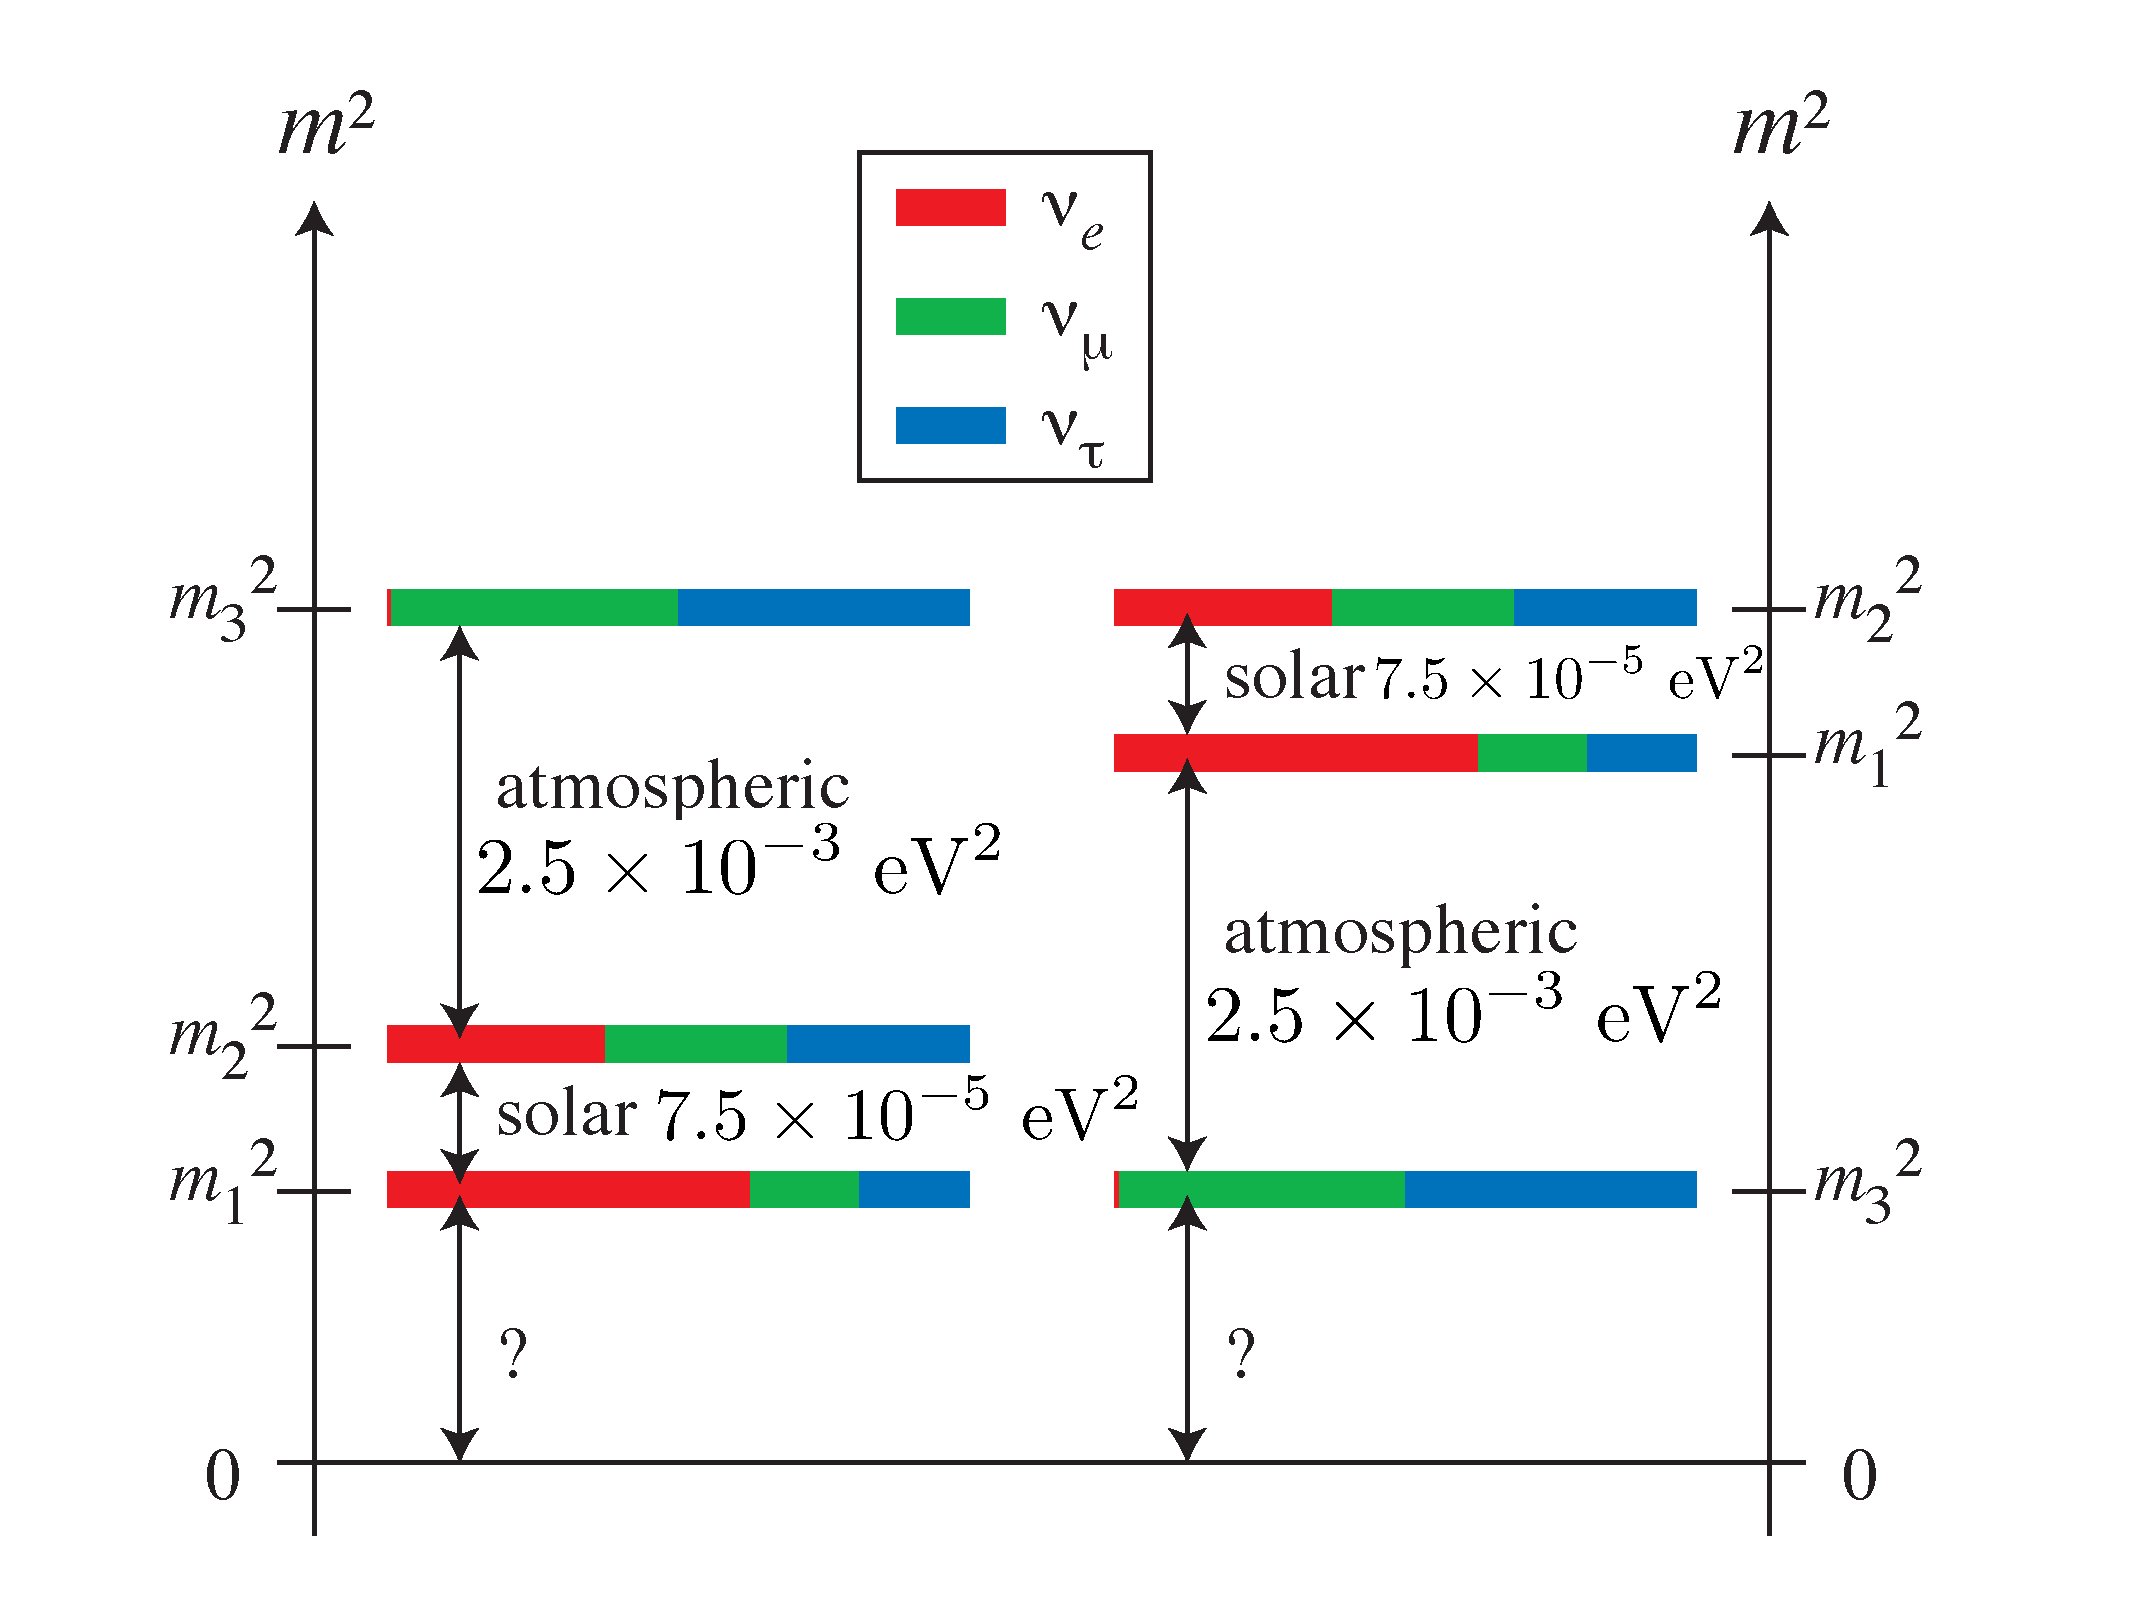
\includegraphics[height=.8\textheight]{nu-detection/mass}
\end{frame}

\begin{frame}{Unknown Parameters}{How to measure them}
	\begin{itemize}
		\item {\color{\emphcol} \dcp}
		\begin{itemize}
			\item[$\Rightarrow$] $P \qty(\HepParticle{\nu}{\alpha}{} \rightarrow \HepParticle{\nu}{\beta}{}) \neq P\qty(\HepAntiParticle{\nu}{\alpha}{} \rightarrow \HepAntiParticle{\nu}{\beta}{})$ for $\theta_{13} \neq 0$
			\item[$\Rightarrow$] Potential explanation for baryon asymmetry via leptogenesis
		\end{itemize}
		\item {\color{\emphcol}$\sgn\qty(\dms_{\m{atm}})$}
		\begin{itemize}
			\item[$\Rightarrow$] Matter effects for non-degenerate value of \dcp
		\end{itemize}
		\item $\alpha_{1,2}$
		\begin{itemize}
			\item[$\Rightarrow$] Only via neutrinoless double beta decay
			\item[$\Rightarrow$] Are \Pgn their own antiparticles?
			\item[$\Rightarrow$] Potential explanation for baryon asymmetry via leptogenesis
		\end{itemize}
	\end{itemize}
\end{frame}

\subsection{Detection}

\begin{frame}{Interaction with Matter}
	\begin{IEEEeqnarray*}{rCl}
		\HepProcess{\Pgnl\Pn \to \Plm\Pp} \\
		\HepProcess{\Pagnl\Pp \to \Plp\Pn}
	\end{IEEEeqnarray*}
	\centering
	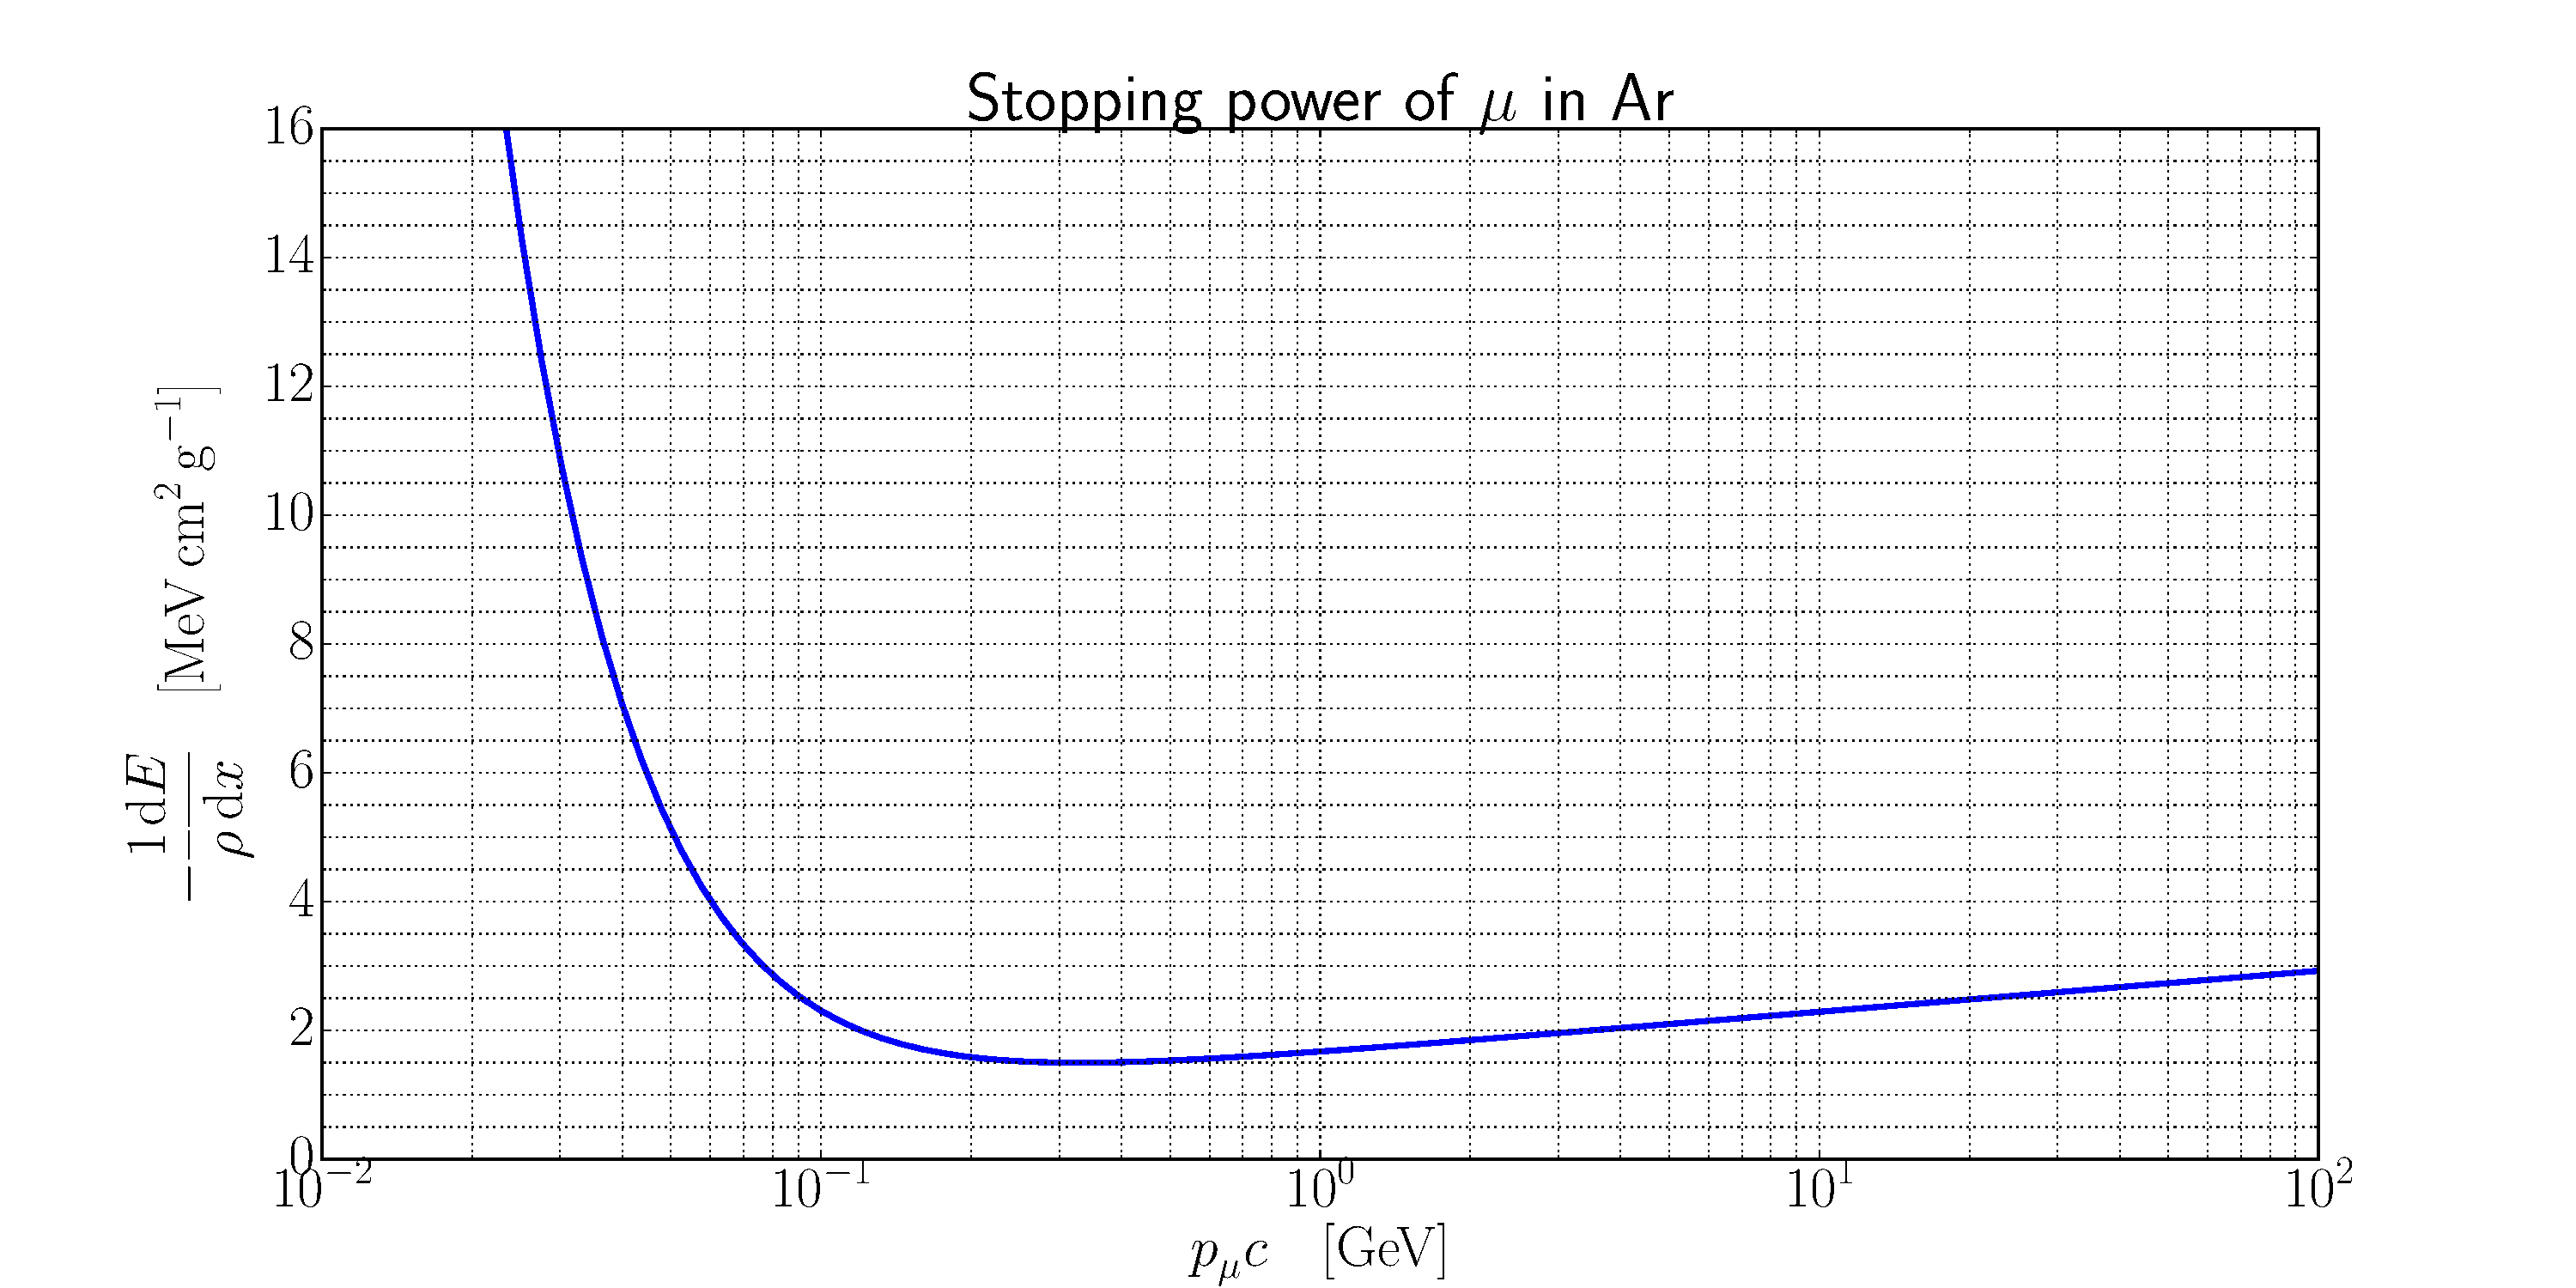
\includegraphics[height=.5\textheight]{nu-detection/bethe_bloch}
	\begin{IEEEeqnarray*}{rCl}
		- \frac{1}{\color{\emphcol} \rho} \dv{E}{x} & = &
		4 \pi N_{\m{A}} r_{\m{e}} ^ 2 m_{\m{e}} c ^ 2 z ^ 2 {\color{\emphcol} \frac{Z}{A}} \frac{1}{\beta ^ 2}
		\qty[\ln(\frac{2 m_{\m{e}} c ^ 2 \gamma ^ 2 \beta ^ 2}{I}) - \beta ^ 2 - \frac{D}{2}]
	\end{IEEEeqnarray*}
\end{frame}

\begin{frame}{Detecting neutrinos}{A challenging task}
	\begin{columns}[c]
		\column{.5\textwidth}
		\centering
		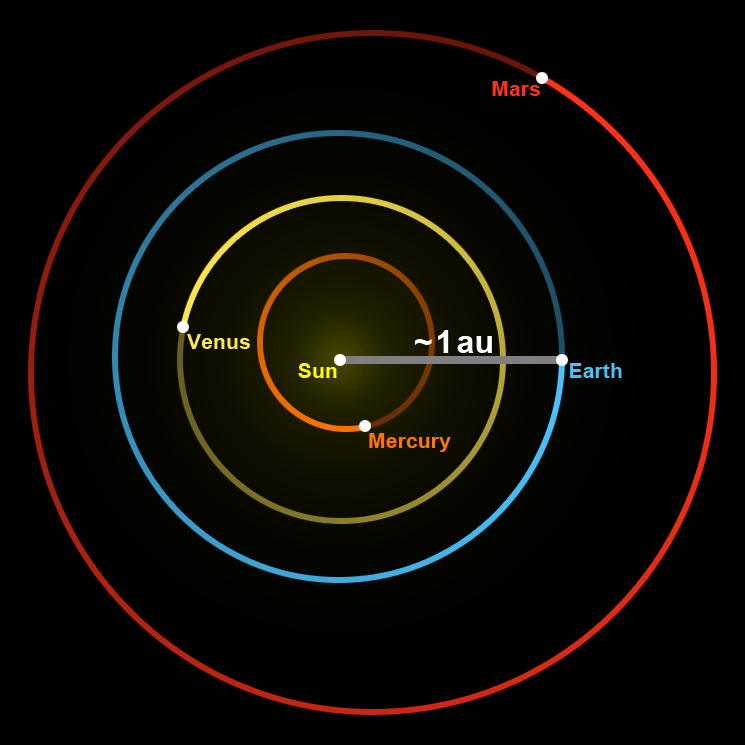
\includegraphics[width=\textwidth]{defence/Astronomical_unit}
		\column{.5\textwidth}
		Detecting a single neutrino would require \SI{\approx 8}{au} of liquid argon.
		This is \num{8} times the distance from the Earth to the Sun.
	\end{columns}
\end{frame}

\begin{frame}{Interaction topologies}{Similar detector response for different topologies $\Rightarrow$ {\color{\emphcol} Need a high-resolution tracker}}
	\begin{columns}[c]
		\column{.5\textwidth}
		\centering
		\begin{fmffile}{fmf/CCQE}
			\unitlength=\textwidth
			\begin{fmfgraph*}(1,.5)
				\fmfpen{thin}
				\fmfstraight
				\fmfleftn{i}{2}
				\fmfrightn{o}{2}
				\fmf{fermion,label=\Pn,label.side=left}{i1,v1}
				\fmf{fermion,label=\Pp,label.side=left}{v1,o1}
				\fmf{fermion,label=\Pgne,label.side=right}{i2,v2}
				\fmf{fermion,label=\Pem,label.side=right}{v2,o2}
				\fmf{boson,label=\PWpm,label.side=left}{v1,v2}
				\fmfdot{v1,v2}
			\end{fmfgraph*}
		\end{fmffile}
		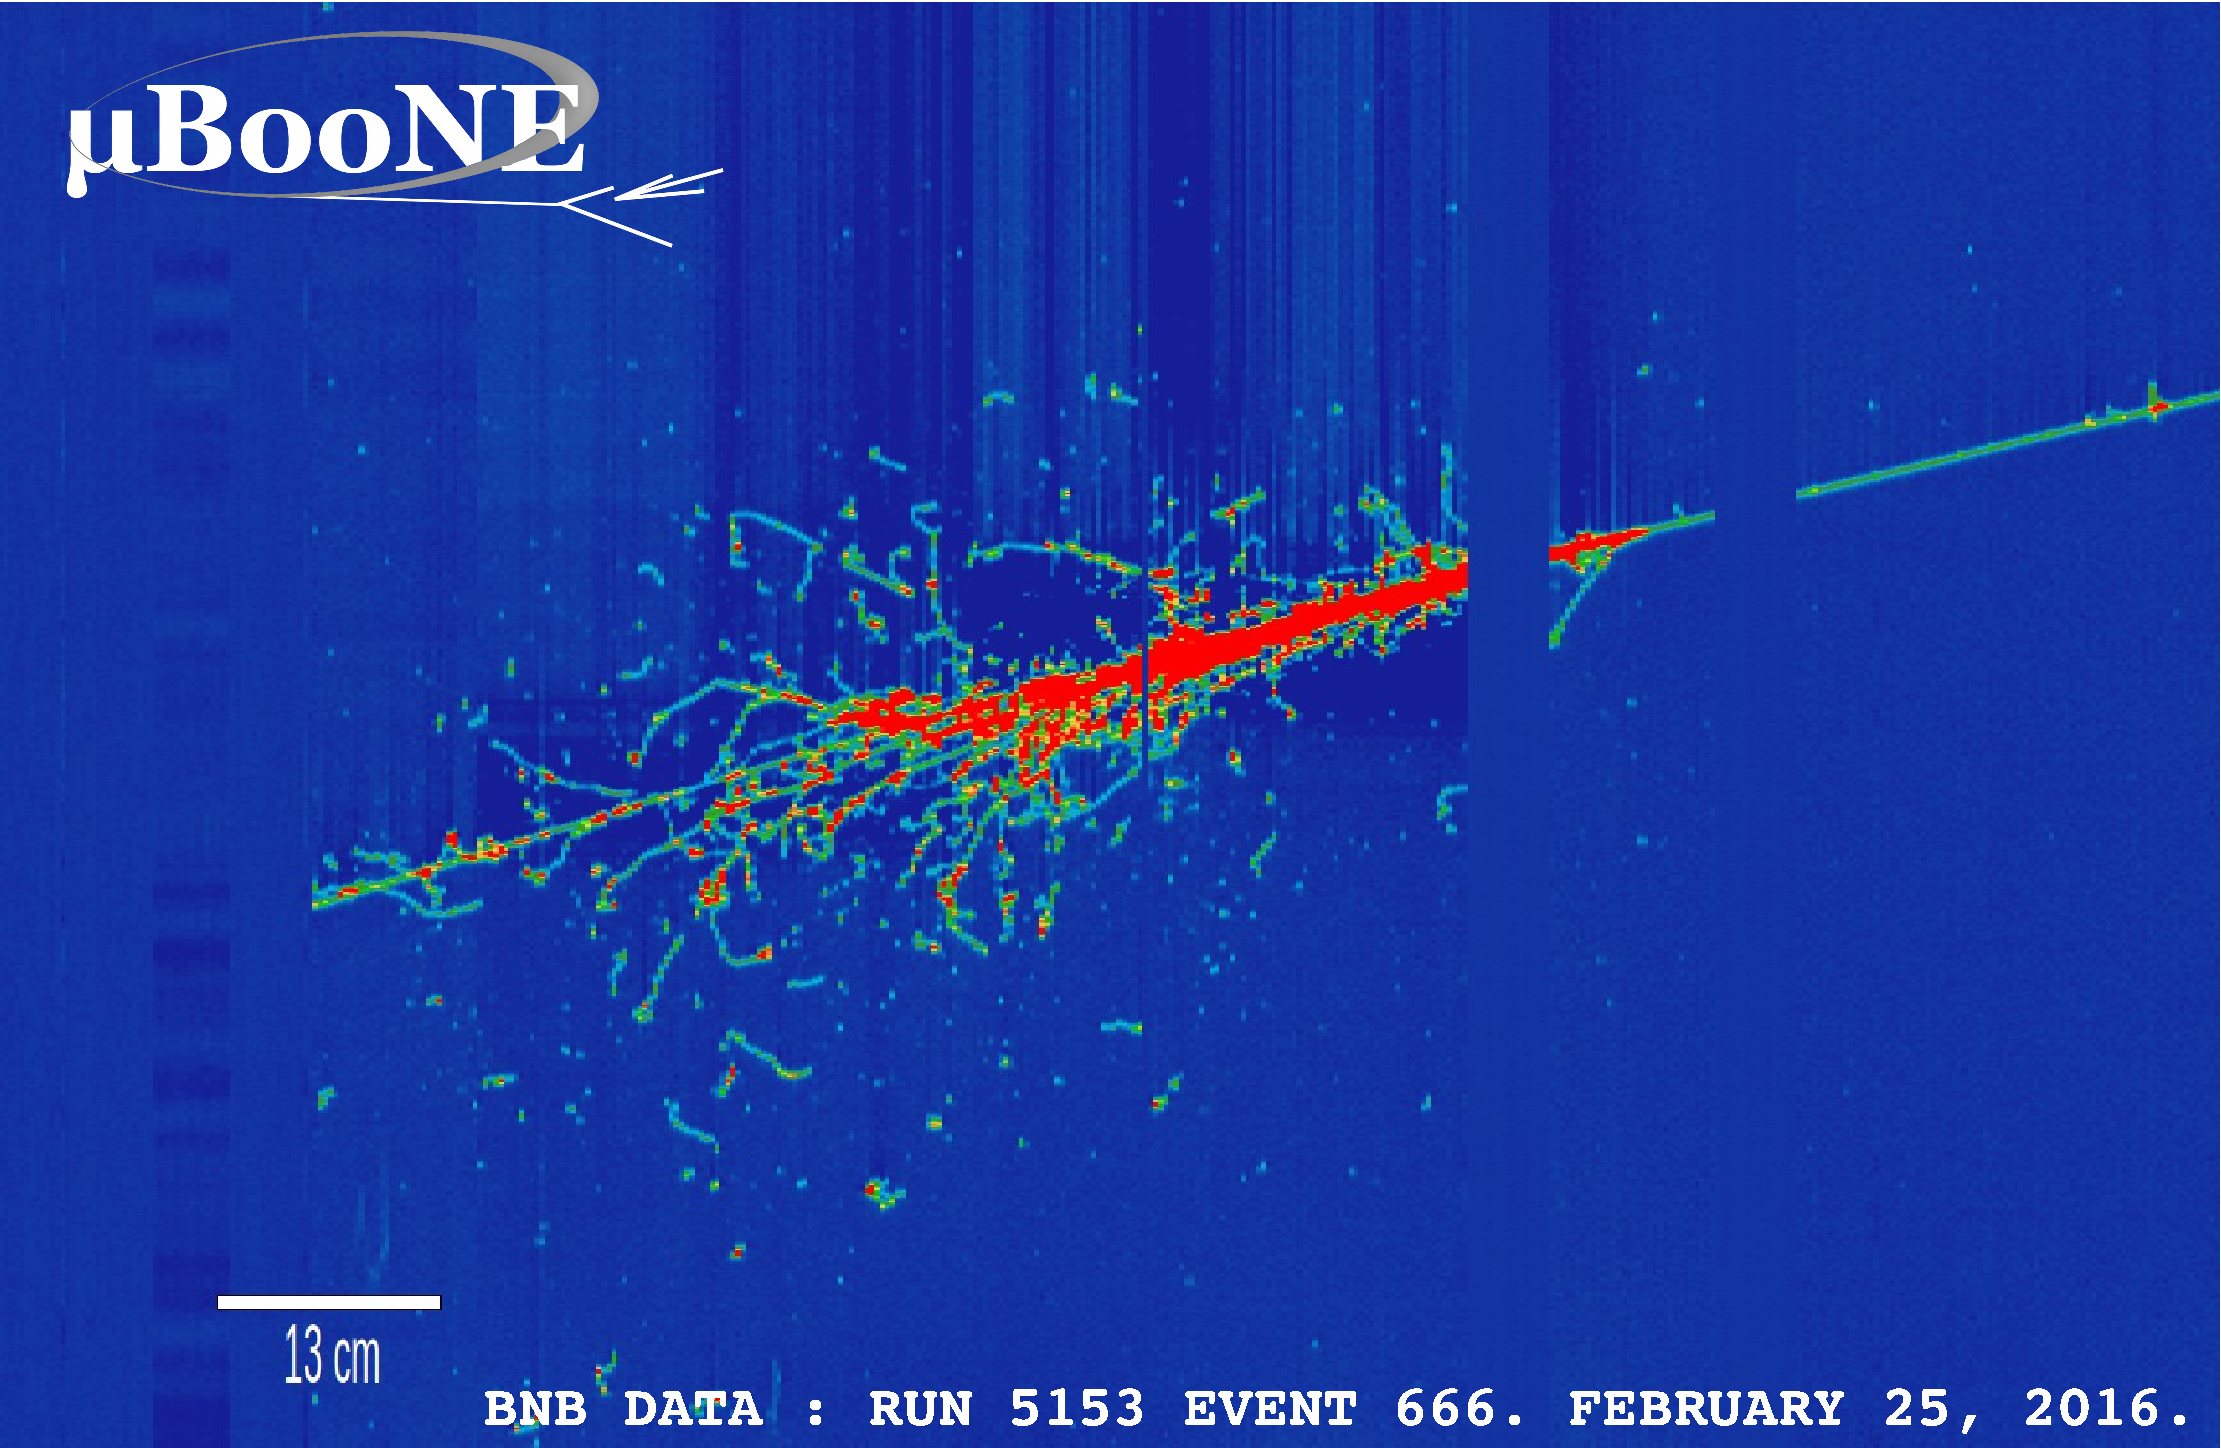
\includegraphics[width=\textwidth]{defence/uboone_em-shower}\\
		\column{.5\textwidth}
		\centering
		\begin{fmffile}{fmf/NCpi0}
			\unitlength=\textwidth
			\begin{fmfgraph*}(1,.5)
				\fmfpen{thin}
				\fmfstraight
				\fmfleftn{i}{2}
				\fmfrightn{o}{4}
				\fmf{heavy,label=\nucleon,label.side=left}{i1,v1,o3}
				\fmf{fermion,label=\Pgpz,label.side=right}{v1,v2}
				\fmf{photon,label=\Pgg,label.side=right}{v2,o1}
				\fmf{photon,label=\Pgg,label.side=left}{v2,o2}
				\fmf{fermion,label=\Pgngm,label.side=right}{i2,v3,o4}
				\fmf{boson,label=\PZz,label.side=left}{v1,v3}
				\fmfdot{v2,v3}
				\fmfblob{20}{v1}
			\end{fmfgraph*}
		\end{fmffile}
		\includegraphics[width=\textwidth]{defence/uboone_em-shower_gamma}\\
	\end{columns}
\end{frame}

\subsection{\dune}

\begin{frame}{Deep Underground Neutrino Experiment (\dune )}{A next generation long-baseline neutrino oscillation experiment}
	\centering
	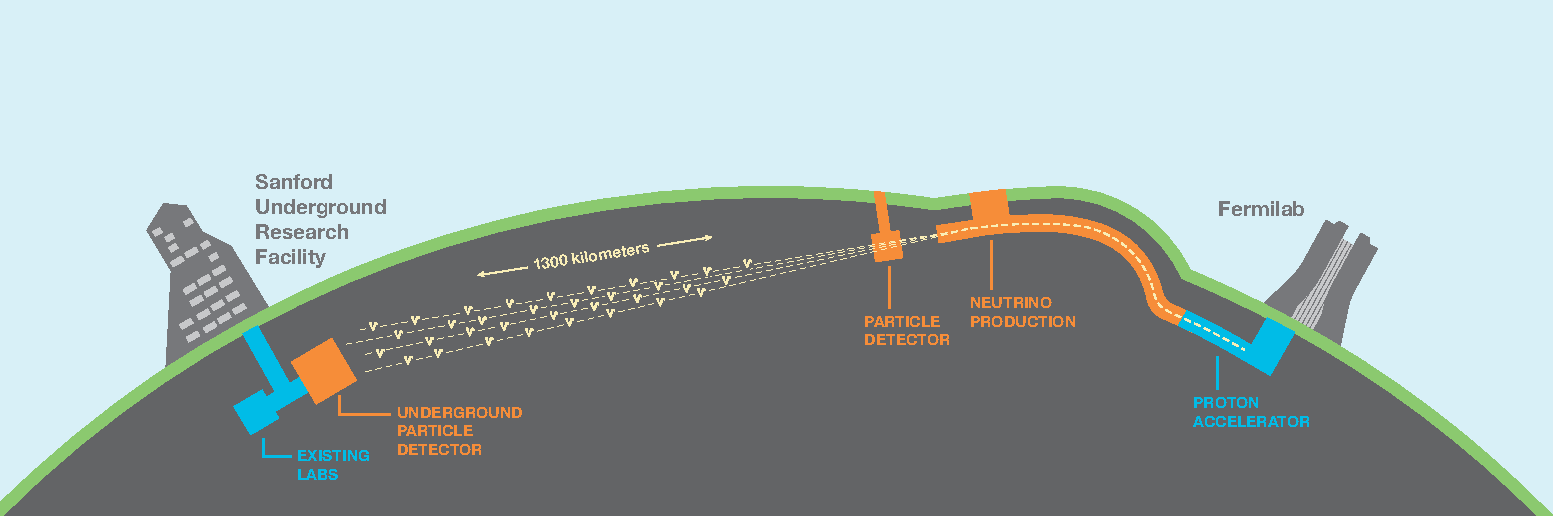
\includegraphics[width=\textwidth]{dune/dune}\\
	{\tiny \dune}\\
	\begin{itemize}
		\item Measure $P\qty(\Pgngm \rightarrow \Pgne)$ and $P\qty(\Pagngm \rightarrow \Pagne) \Rightarrow$ {\color{\emphcol}$\dcp$, $\sgn\qty(\dms_{\m{atm}})$}
		\item High intensity \Pgngm/\Pagngm beam from Fermilab
		\item Near detector @ \SI{0.574}{\kilo\metre} baseline
		\item \SI{40}{\kilo\tonne} \lartpc\ far detector @ \SI{1300}{\kilo\metre} baseline
	\end{itemize}
\end{frame}

\begin{frame}{Interaction cross sections vs.\ beam flux}
	\begin{columns}[c]
		\column{.6\textwidth}
		\centering
		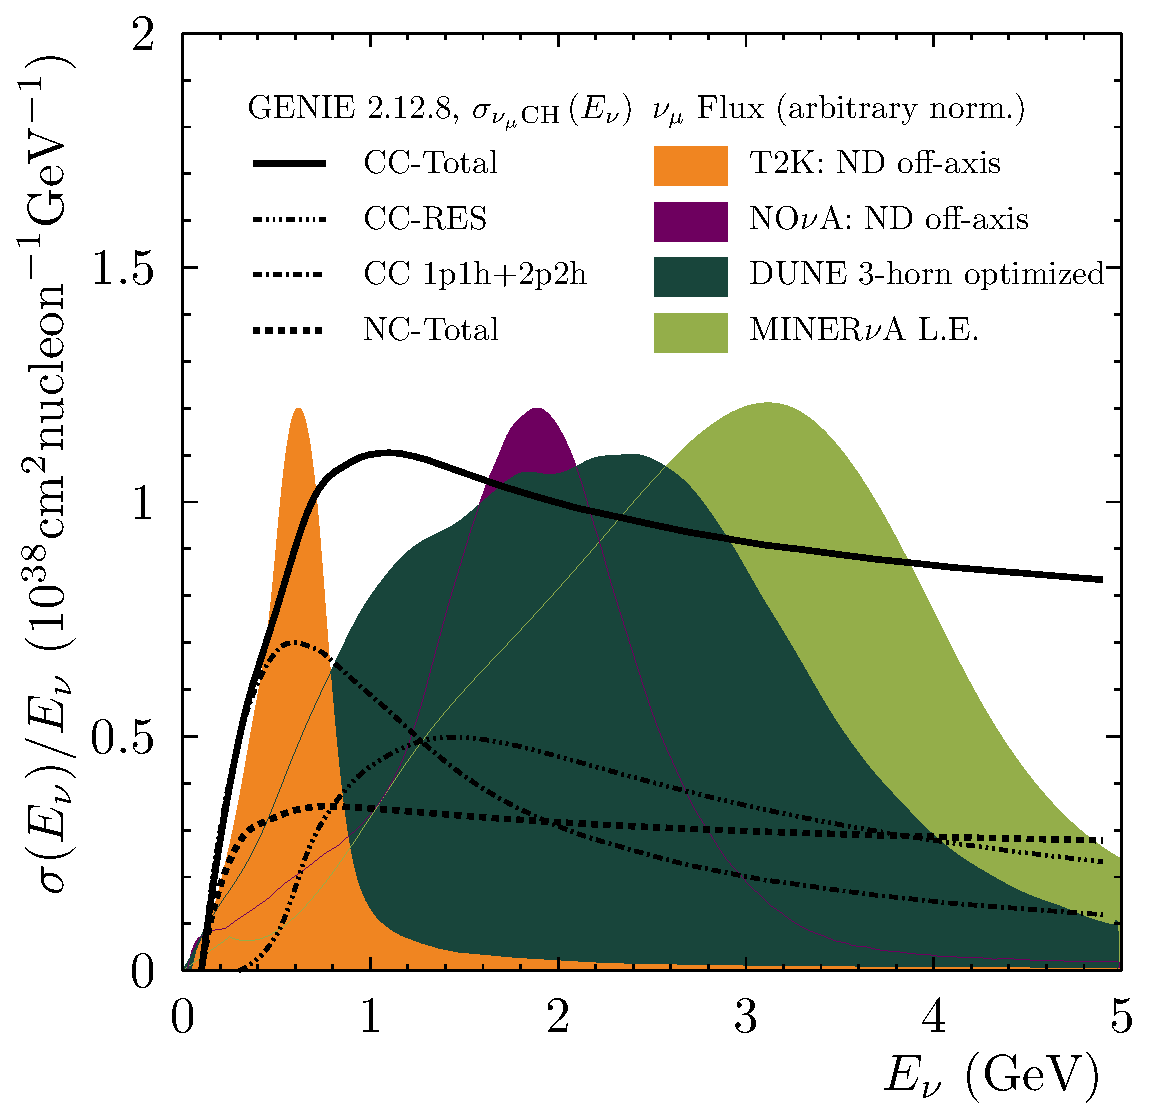
\includegraphics[width=\textwidth]{nu-detection/flux_and_xsec_from_luke}\\
		{\tiny L.\ Pickering}\\
		\column{.4\textwidth}
		{\color{\emphcol} $\sigma \sim \SI{e-38}{\centi\metre\squared}$}
		\begin{itemize}
			\item[$\Rightarrow$] High target mass
			\item[$\Rightarrow$] High flux
		\end{itemize}
		{\color{\emphcol} \dune{} flux peak \SI{\approx 2.5}{\giga\electronvolt}}
	\end{columns}
\end{frame}

\begin{frame}{Sensitivity}
	\begin{columns}[c]
		\column{.5\textwidth}
		\centering
		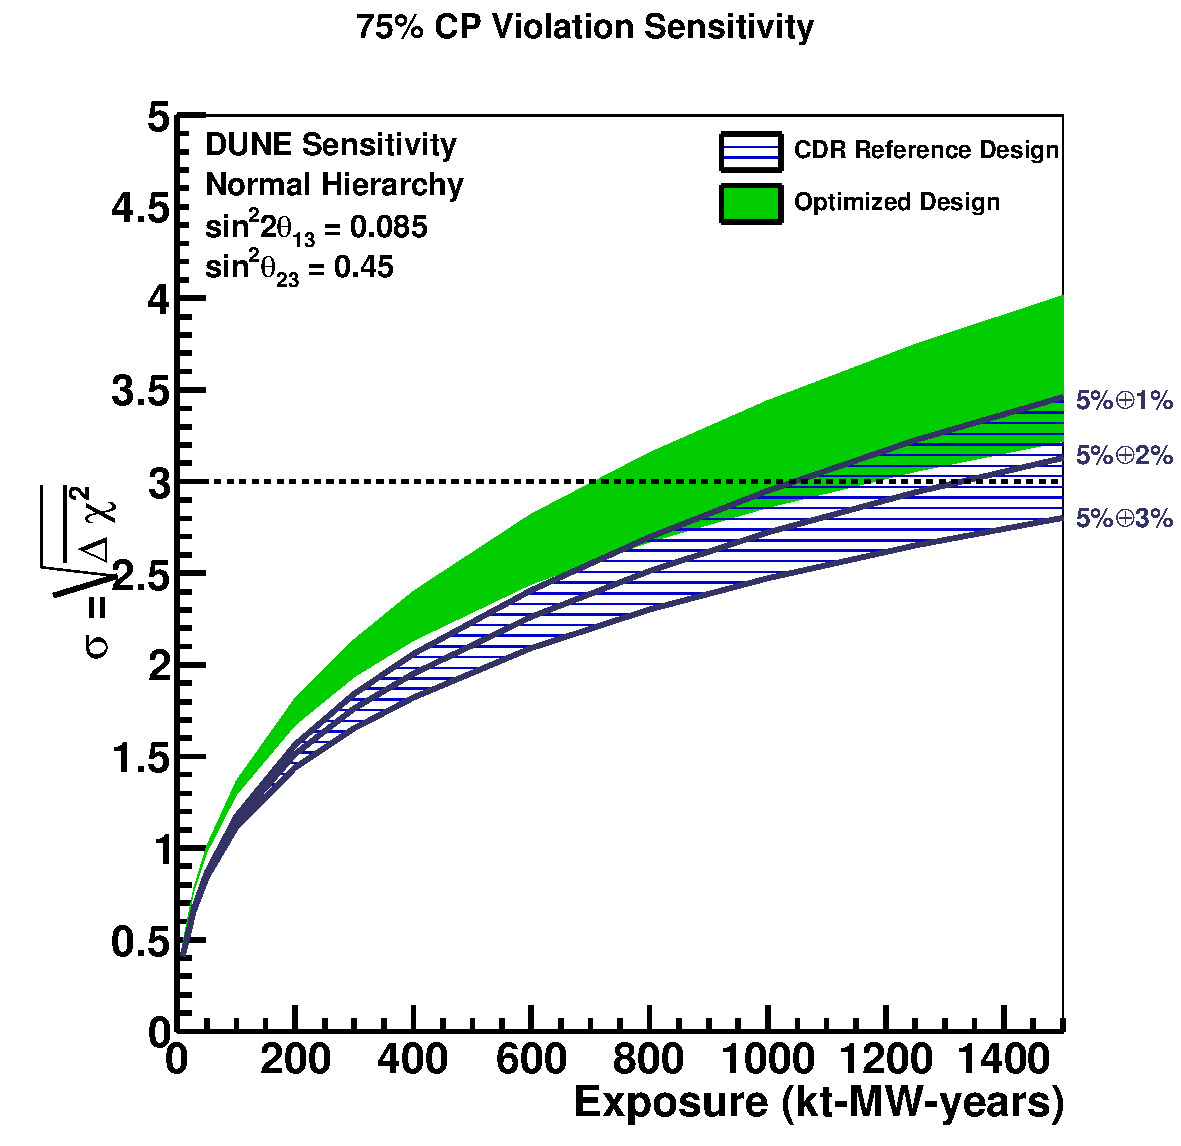
\includegraphics[width=\textwidth]{dune/cpv75_exp_syst}\\
		{\tiny \dune\ arXiv:~1512.06148~\cite{dune}}\\
		\num{25} years with \SI{40}{\kilo\tonne}\\
		{\color{\emphcol} $\Rightarrow$ need beam intensity $> \SI{1}{\mega\watt}$}\\
		\column{.5\textwidth}
		\SI{75}{\percent} CP violation coverage at $\num{3}\sigma$ requires beam related uncorrelated uncertainties $< \SI{2}{\percent}$.\\
		{\color{\emphcol} Constraining beam at near detector} requires
		\begin{itemize}
			\item High statistics
			\item High resolution
			\item[$\Rightarrow$] Good background rejection
			\item Ideally, same material and technology as far detector
			\item[$\Rightarrow$] Cancel uncertainties on
			\begin{itemize}
				\item Cross section
				\item Detector response
			\end{itemize}
		\end{itemize}
	\end{columns}
\end{frame}

\begin{frame}{Challenges for the near detector}{High multiplicities}
	\begin{itemize}
		\item Simulation of a single neutrino beam spill, including backgrounds
		\item {\color{\emphcol} \num{0.2} beam events per tonne @ \SI{2}{\mega\watt}}
	\end{itemize}
	\centering
	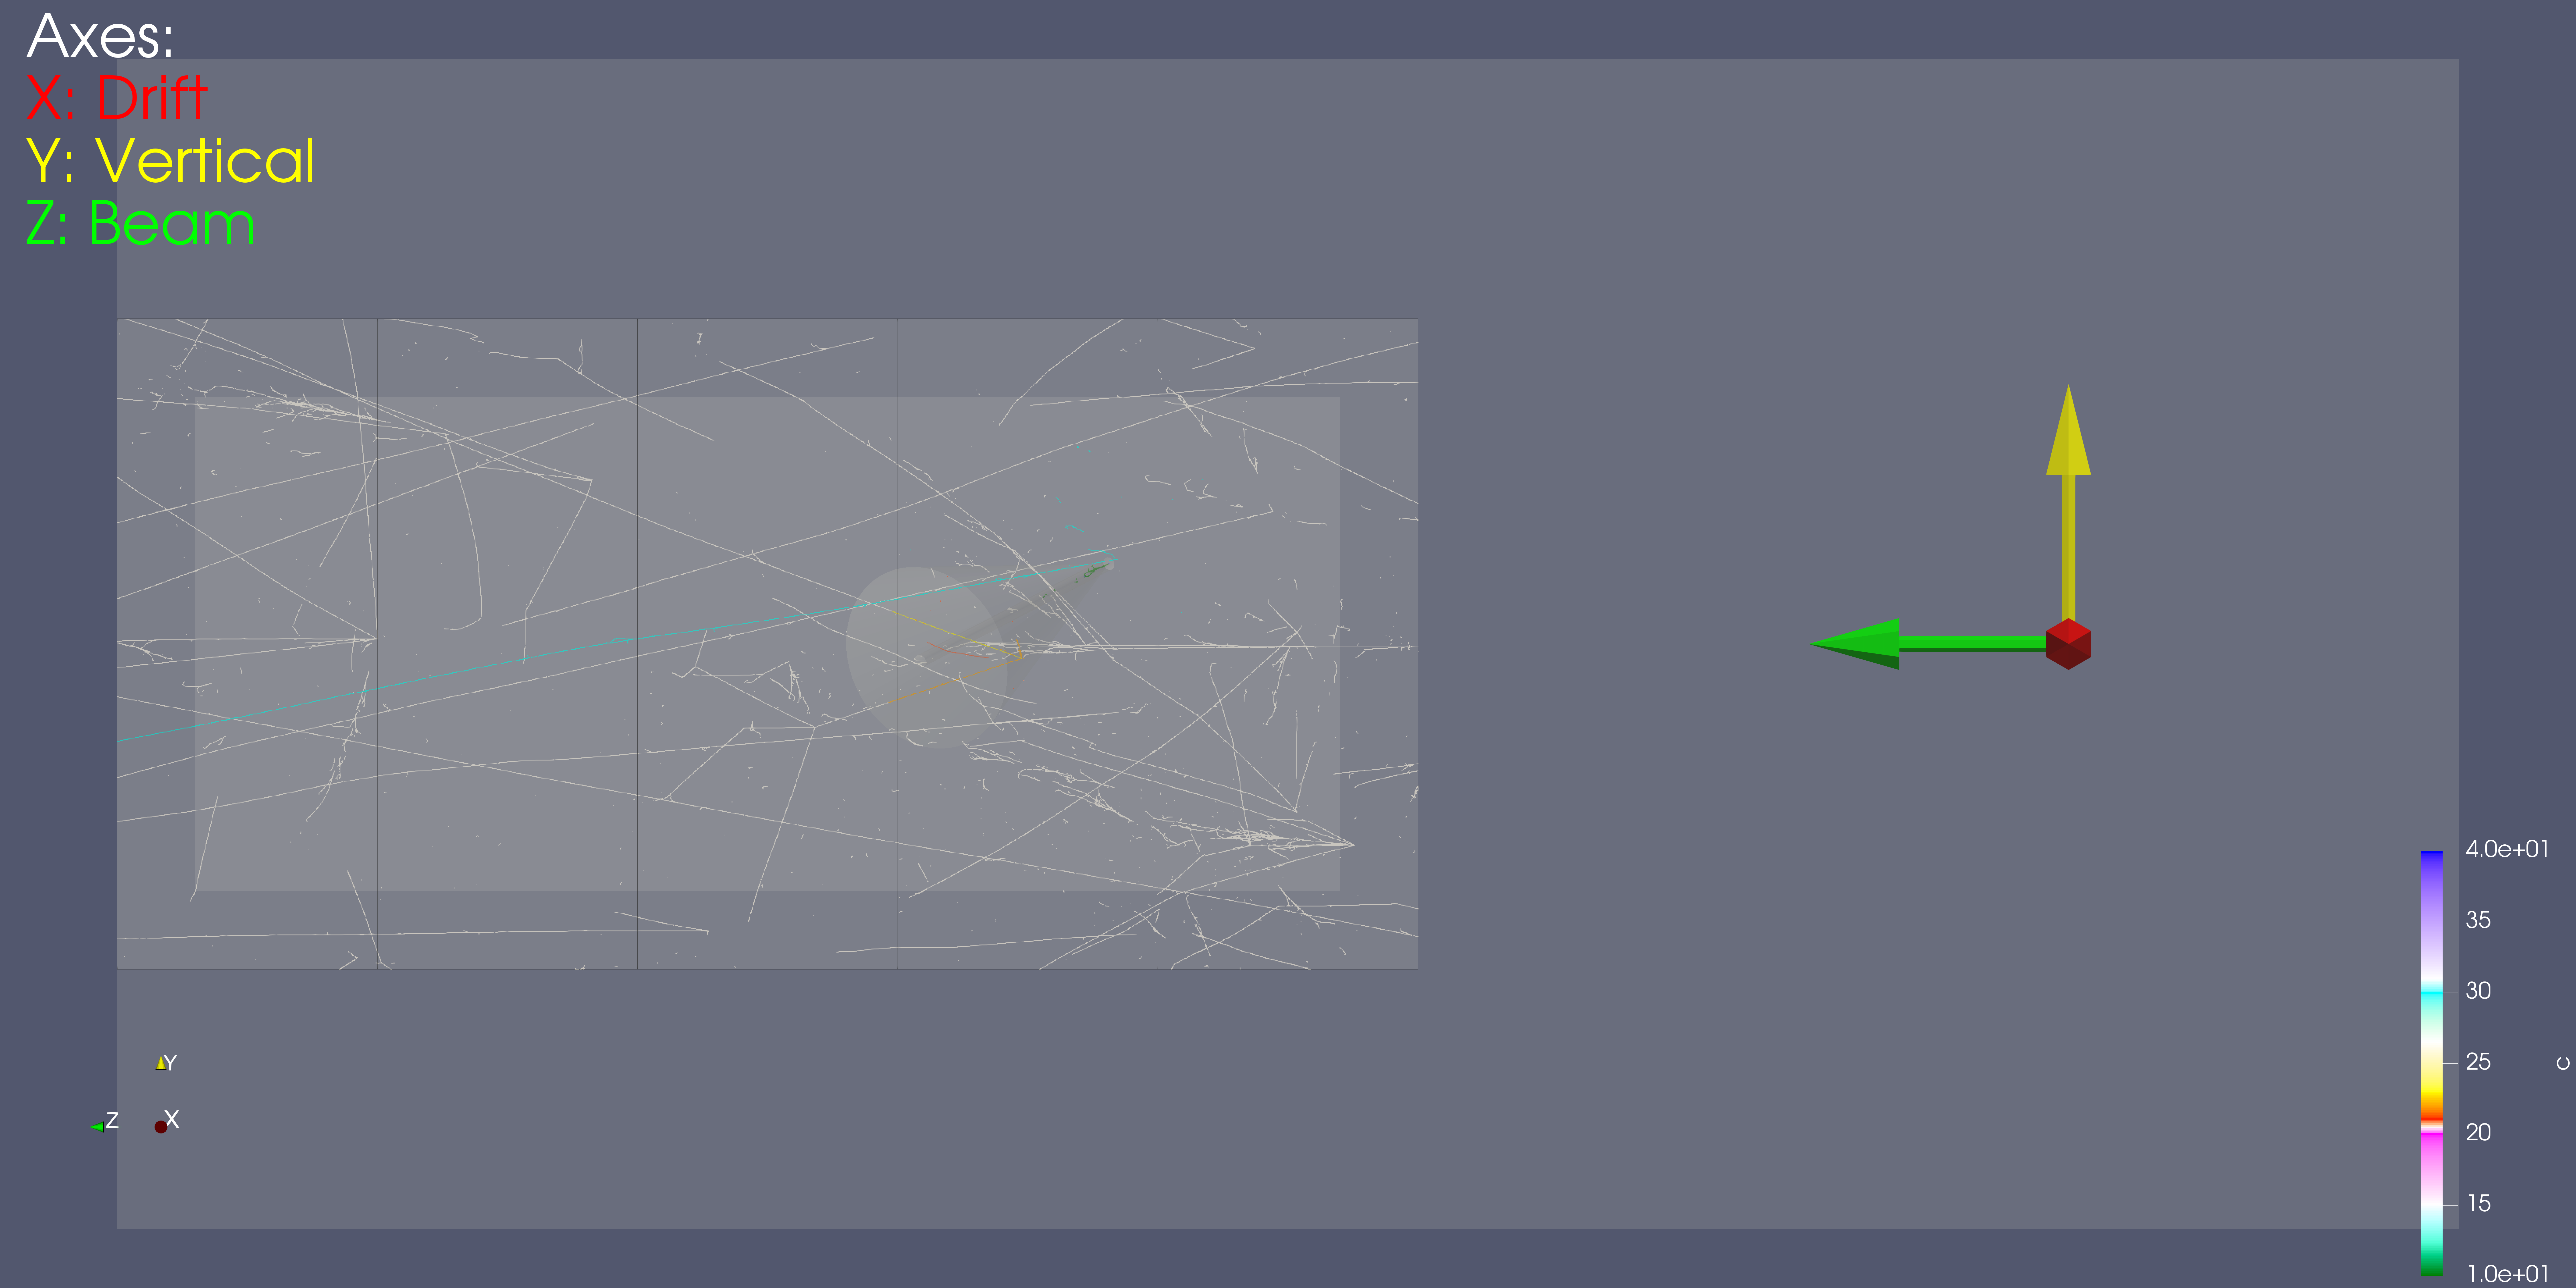
\includegraphics[viewport=407 1112 4956 3389, clip, width=\textwidth]{pile-up/uid0_spill6_event461_gamma19_x}
\end{frame}

\begin{frame}{Neutrino physics summary}{Neutrino detection is hard}
	\begin{enumerate}
		\item High beam flux
		\item High target mass
		\item High-precision tracking
		\item High-precision calorimetry
	\end{enumerate}
	{\color{\emphcol}A \lartpc{} provides \numrange{2}{4}.\\Theoretically...}
\end{frame}

\section{The \lartpc{}}

\begin{frame}{The time projection chamber (TPC)}{A detector providing precise tracking and calorimetry}
	\centering
	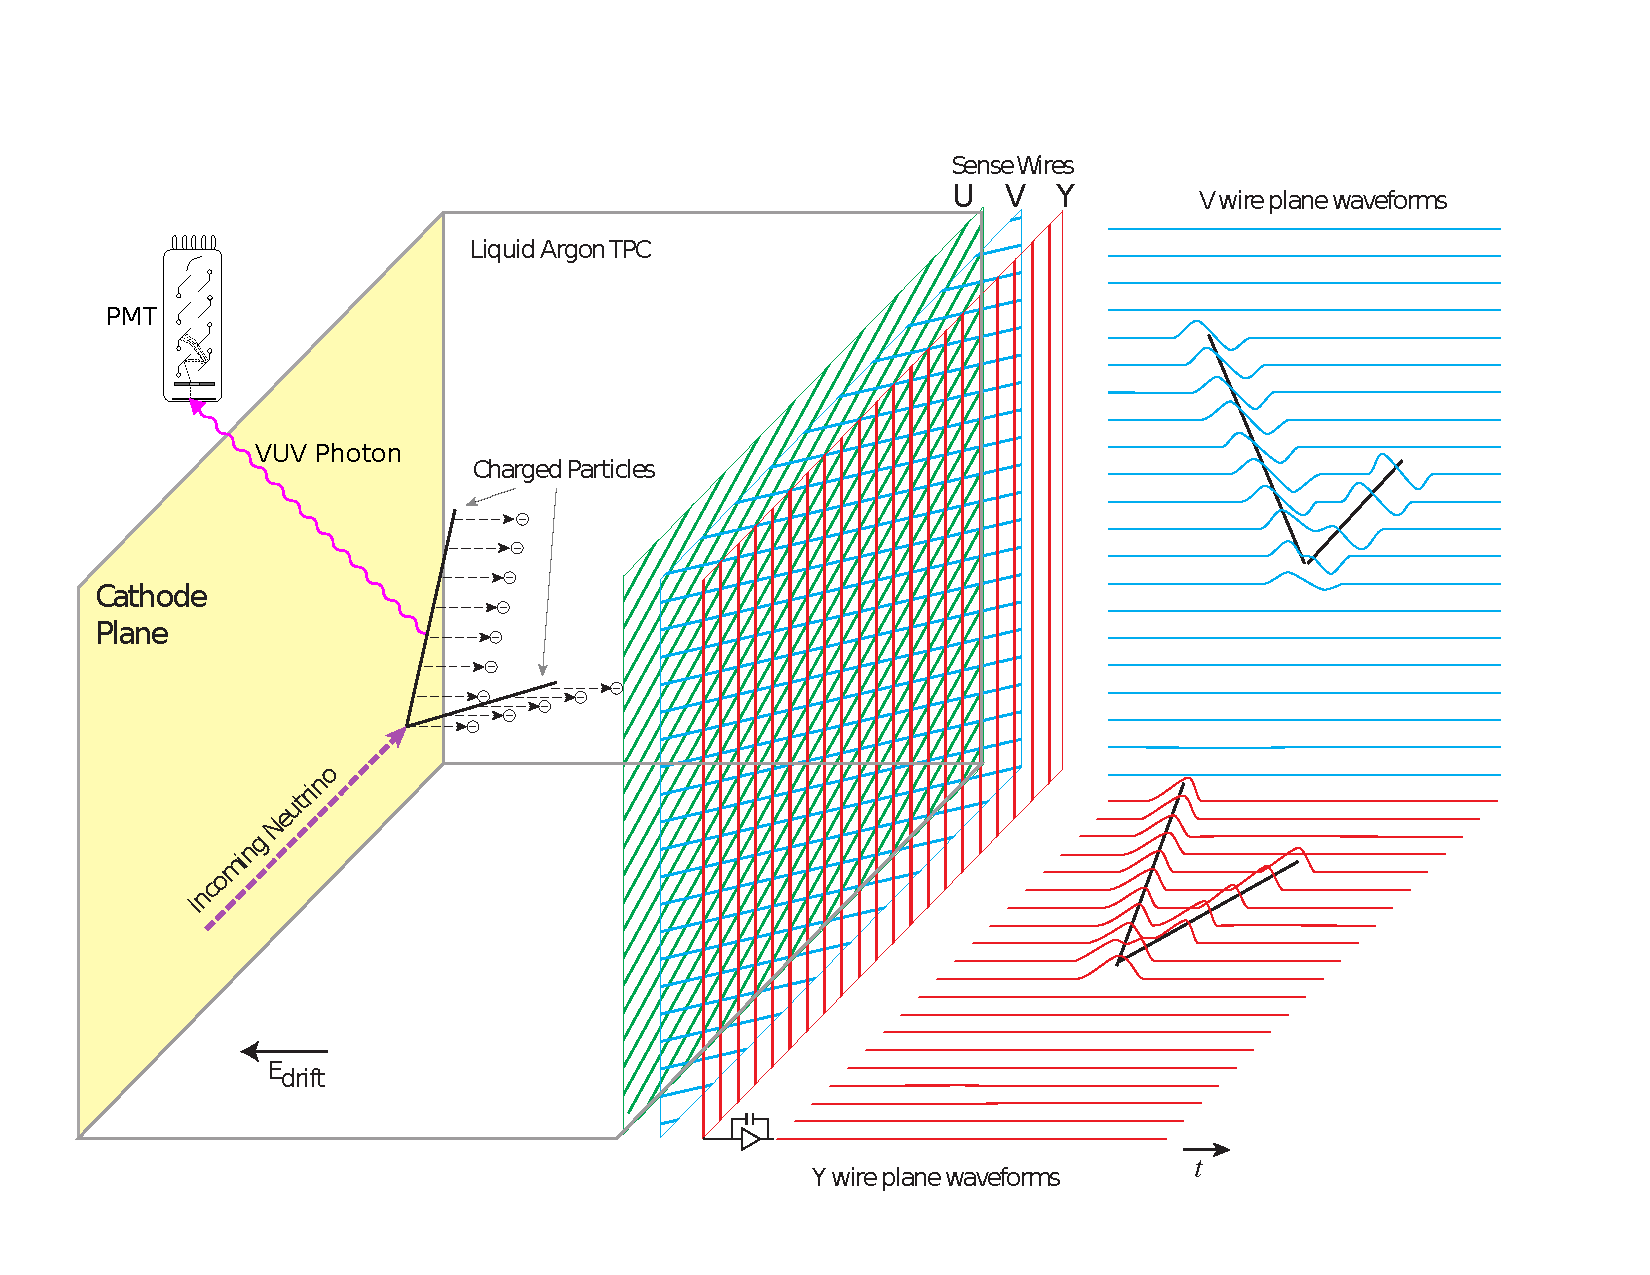
\includegraphics[viewport=35 40 720 540, clip, height=.66\textheight]{defence/TPCprinciple}\\
	{\tiny \uboone{} arXiv:~1612.05824~\cite{uboone}}\\
\end{frame}

\begin{frame}{Why liquid argon?}
	\begin{columns}[c]
		\column{.3\textwidth}
		\centering
		
\includegraphics[width=\textwidth]{defence/ArTube}
		\column{.7\textwidth}
		\begin{itemize}
			\item Dense (\SI{1.4e3}{\kilo\gram\per\cubic\metre}) \emph{$\rightarrow$ high event rate}
			\item Abundant (\SI{\approx 1}{\percent} of the Earth's atmosphere) \emph{$\rightarrow$ cheap}
			\item High ionisation yield (\SI{8900}{\elementarycharge\per\milli\metre} for a MIP) \emph{$\rightarrow$ tracking \& calorimetry}
			\item Prompt scintillation ($\sim \si{\nano\second}$) \emph{$\rightarrow$ tracking (absolute spatial reference)}
			\item Liquid @ \SI{87}{\kelvin}
			\item Drift speed @ \SI{0.1}{\kilo\volt\per\milli\meter} \SI{\approx 2}{\milli\meter\per\micro\second}
		\end{itemize}
		{\color{\emphcol} Meets all the requirements for neutrino detection with a TPC}
	\end{columns}
\end{frame}

\section{Drift field generation}

\begin{frame}{The standard \lartpc{} design}{Drift field generation}
	\centering
	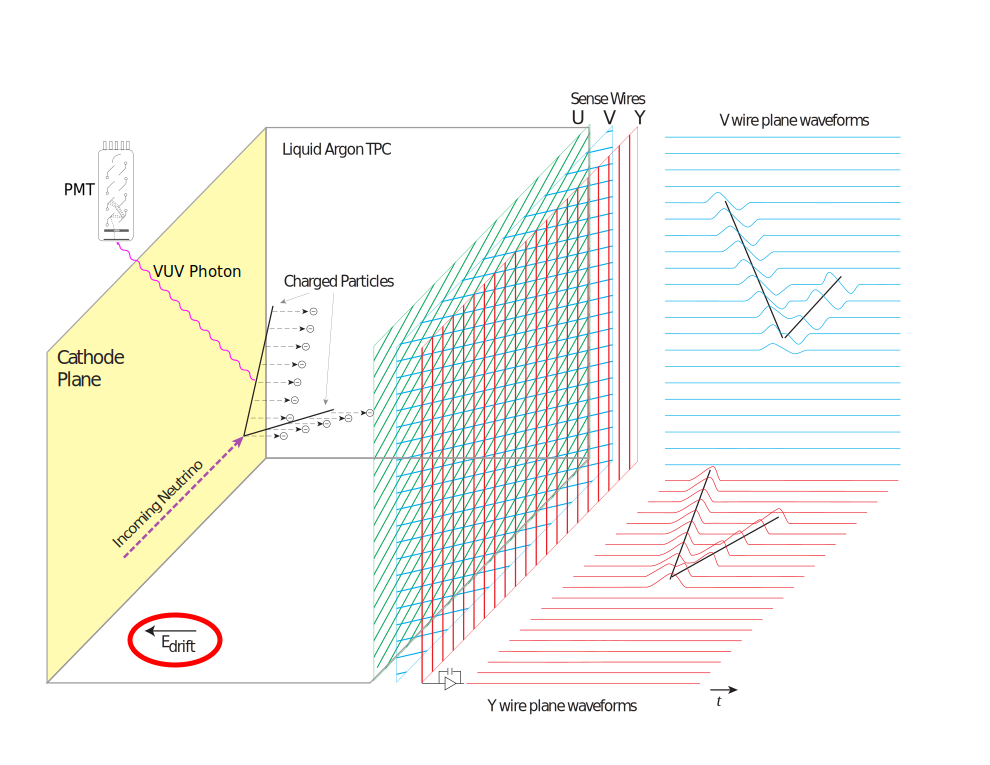
\includegraphics[viewport=35 40 720 540, clip, height=.66\textheight]{defence/TPCprinciple_HV}\\
	{\tiny \uboone{} arXiv:~1612.05824~\cite{uboone}}\\
\end{frame}

\begin{frame}{Dielectric strength of liquid argon}{\color{\emphcol} Lower than expected}
	\begin{columns}[c]
		\column{.5\textwidth}
		\centering
		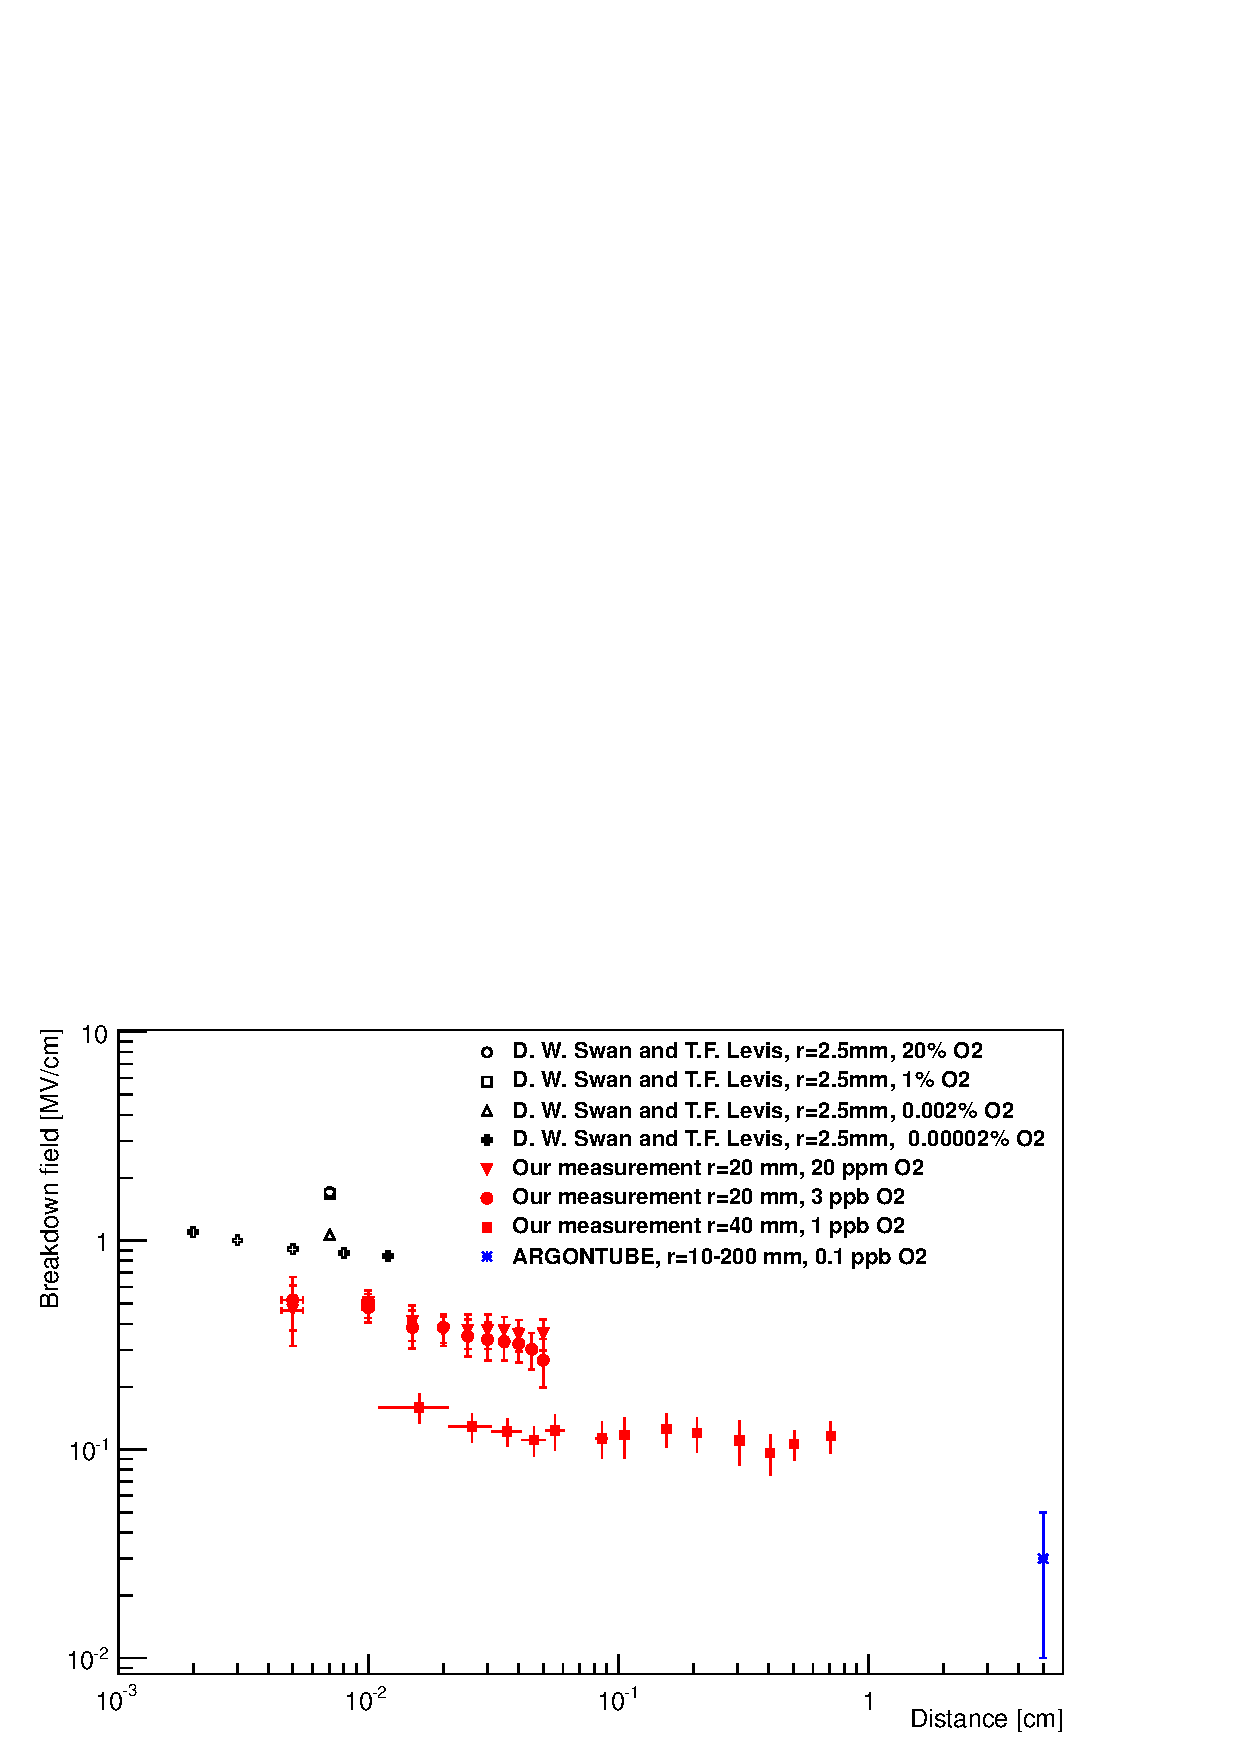
\includegraphics[viewport=18 10 511 351, clip, width=\textwidth]{defence/breakdown_plot}
		\column{.5\textwidth}
		\centering
		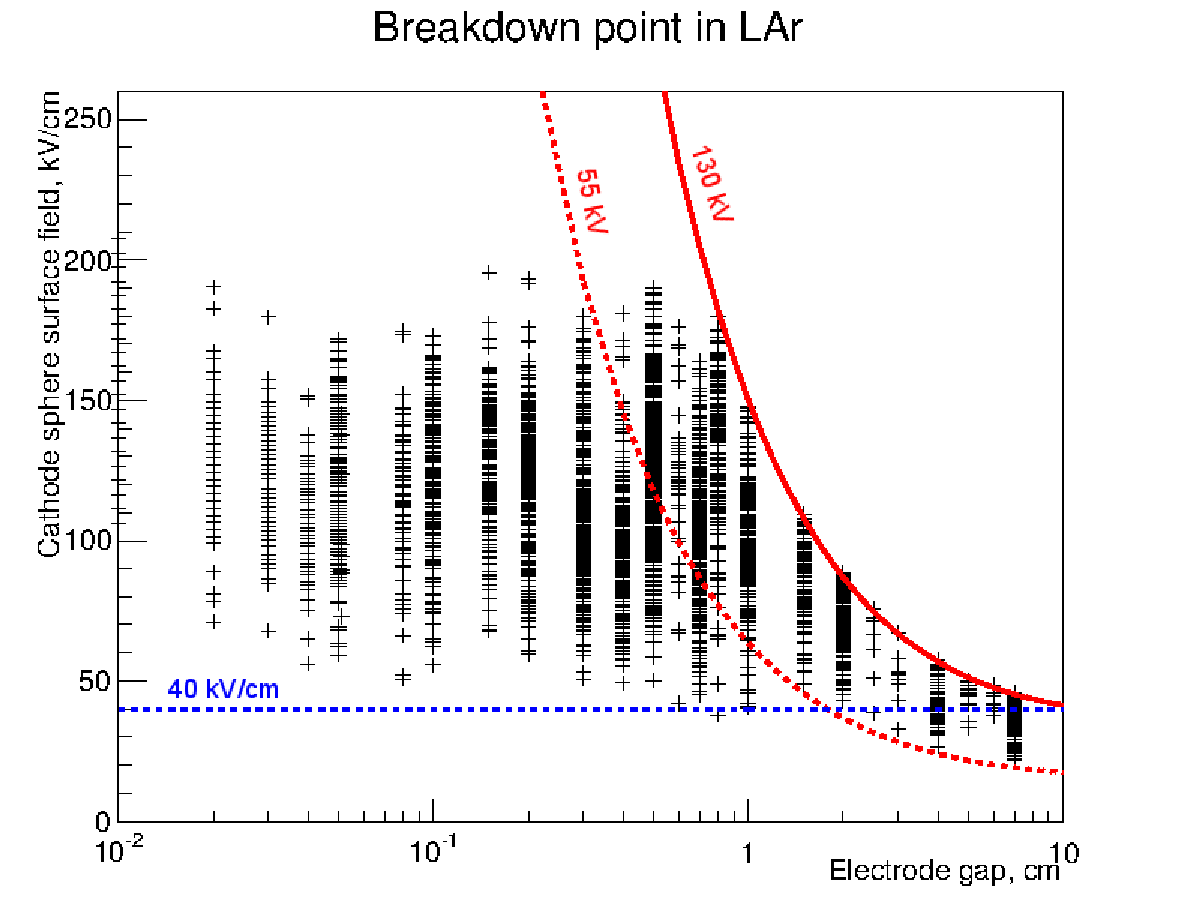
\includegraphics[width=\textwidth]{defence/breakdown_summary}
	\end{columns}
	\centering
	{\tiny Blatter et al.\ arXiv:~1401.6693~\cite{breakdown_14}}\\
\end{frame}

\begin{frame}{Footage of a typical breakdown}{Animated version of another breakdown: \url{http://tinyurl.com/y872x4oq}}
	\centering
	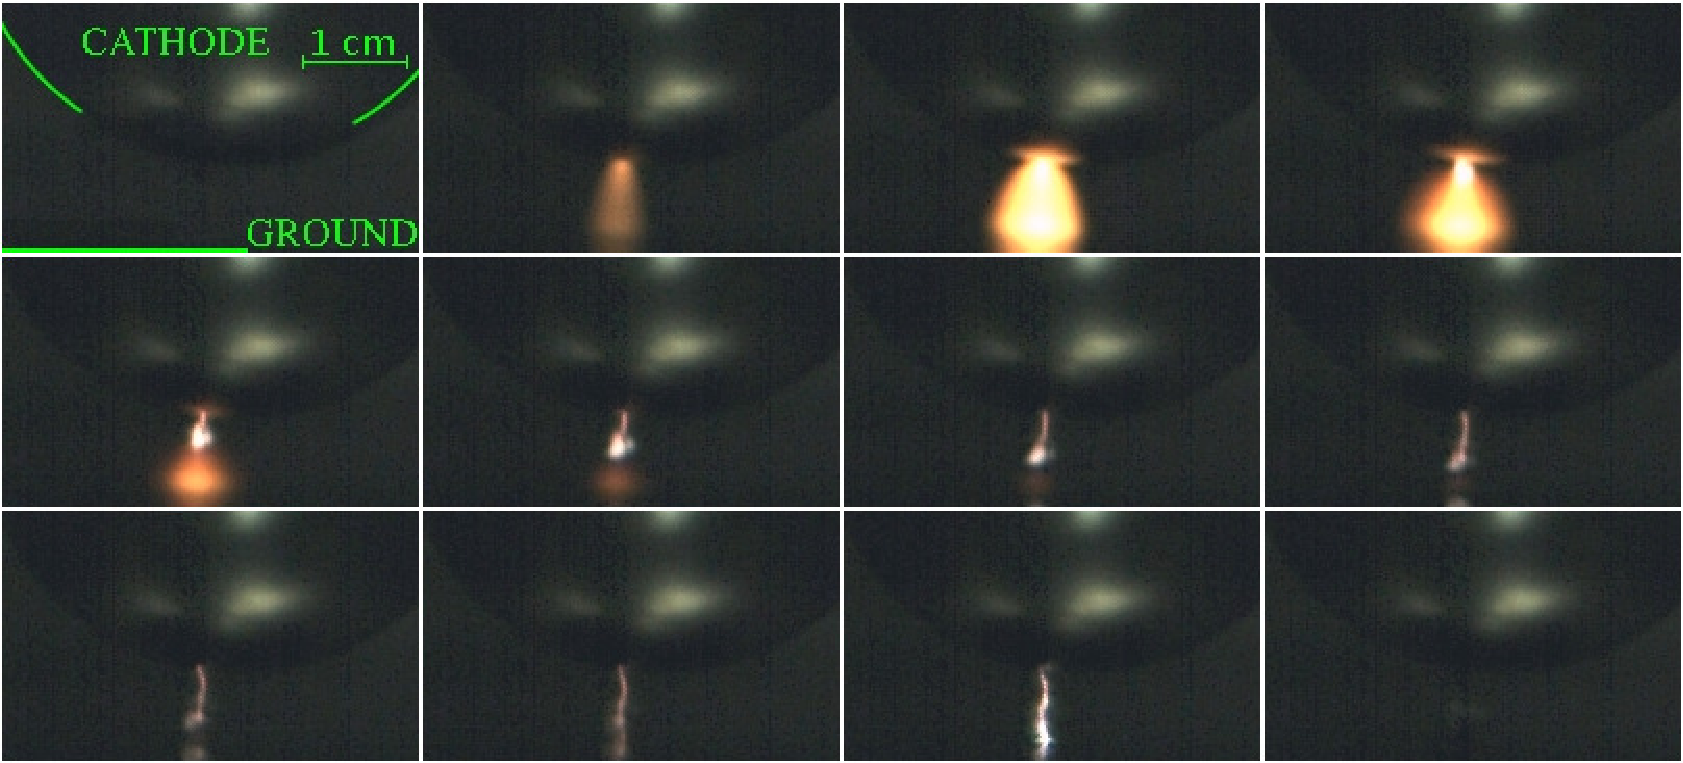
\includegraphics[width=\textwidth]{hv/montage}\\
	{\tiny Auger, Goeldi et al.\ arXiv:~1512.05968~\cite{breakdown_16}}\\
\end{frame}

\begin{frame}{Current voltage behaviour of a typical breakdown}{\color{\emphcol} Rather slow process}
	\centering
	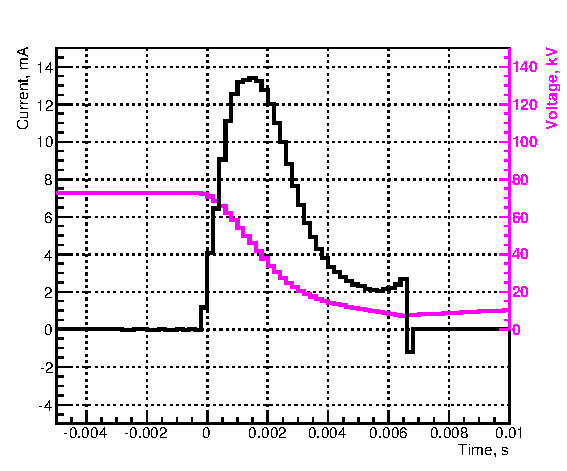
\includegraphics[height=.75\textheight]{hv/IVcorr}\\
	{\tiny Auger, Goeldi et al.\ arXiv:~1512.05968~\cite{breakdown_16}}\\
\end{frame}

\begin{frame}{Preventing breakdowns}{with a polymer coating}
	\begin{columns}[c]
		\column{.5\textwidth}
		\begin{itemize}
			\item low electron mobility
			\item slightly conducting
		\end{itemize}
		\column{.5\textwidth}
		\begin{itemize}
			\item {\color{\emphcol} only single-use}
		\end{itemize}
	\end{columns}
	\begin{columns}[c]
		\column{.333\textwidth}
		\centering
		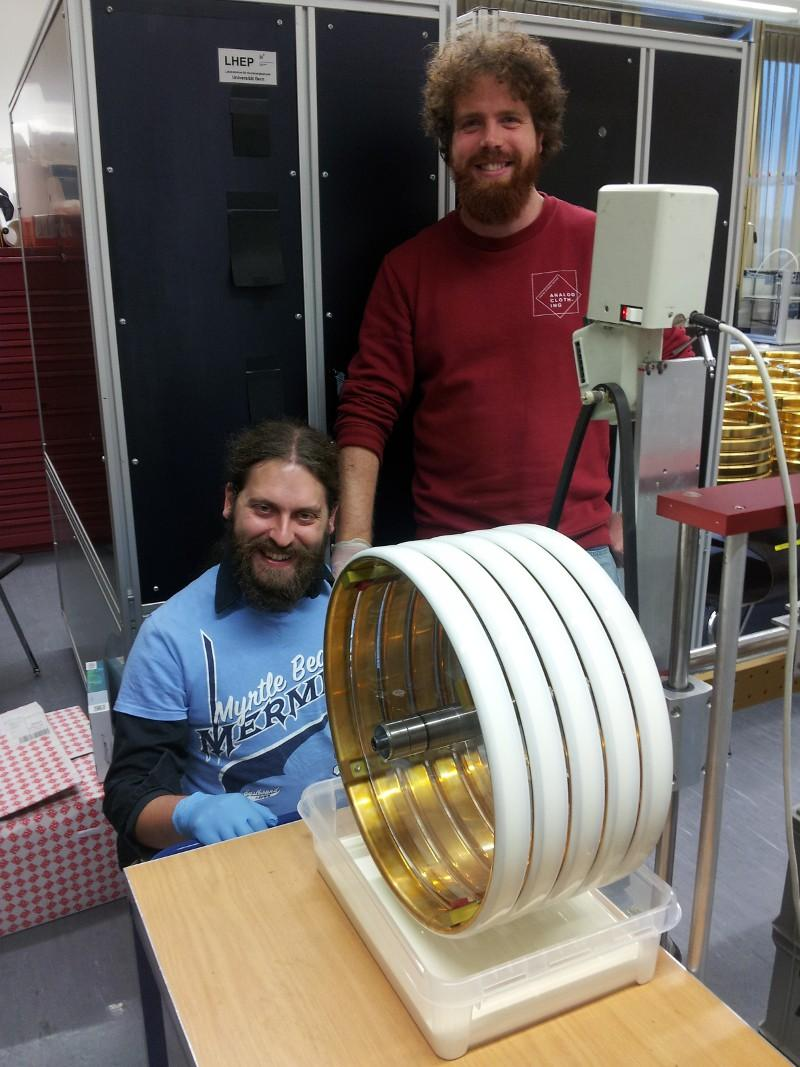
\includegraphics[width=\textwidth]{defence/coating}
		\column{.333\textwidth}
		\centering
		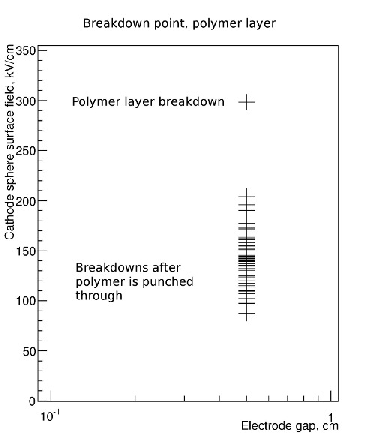
\includegraphics[width=\textwidth]{defence/breakdown_latex}
		\column{.333\textwidth}
		\centering
		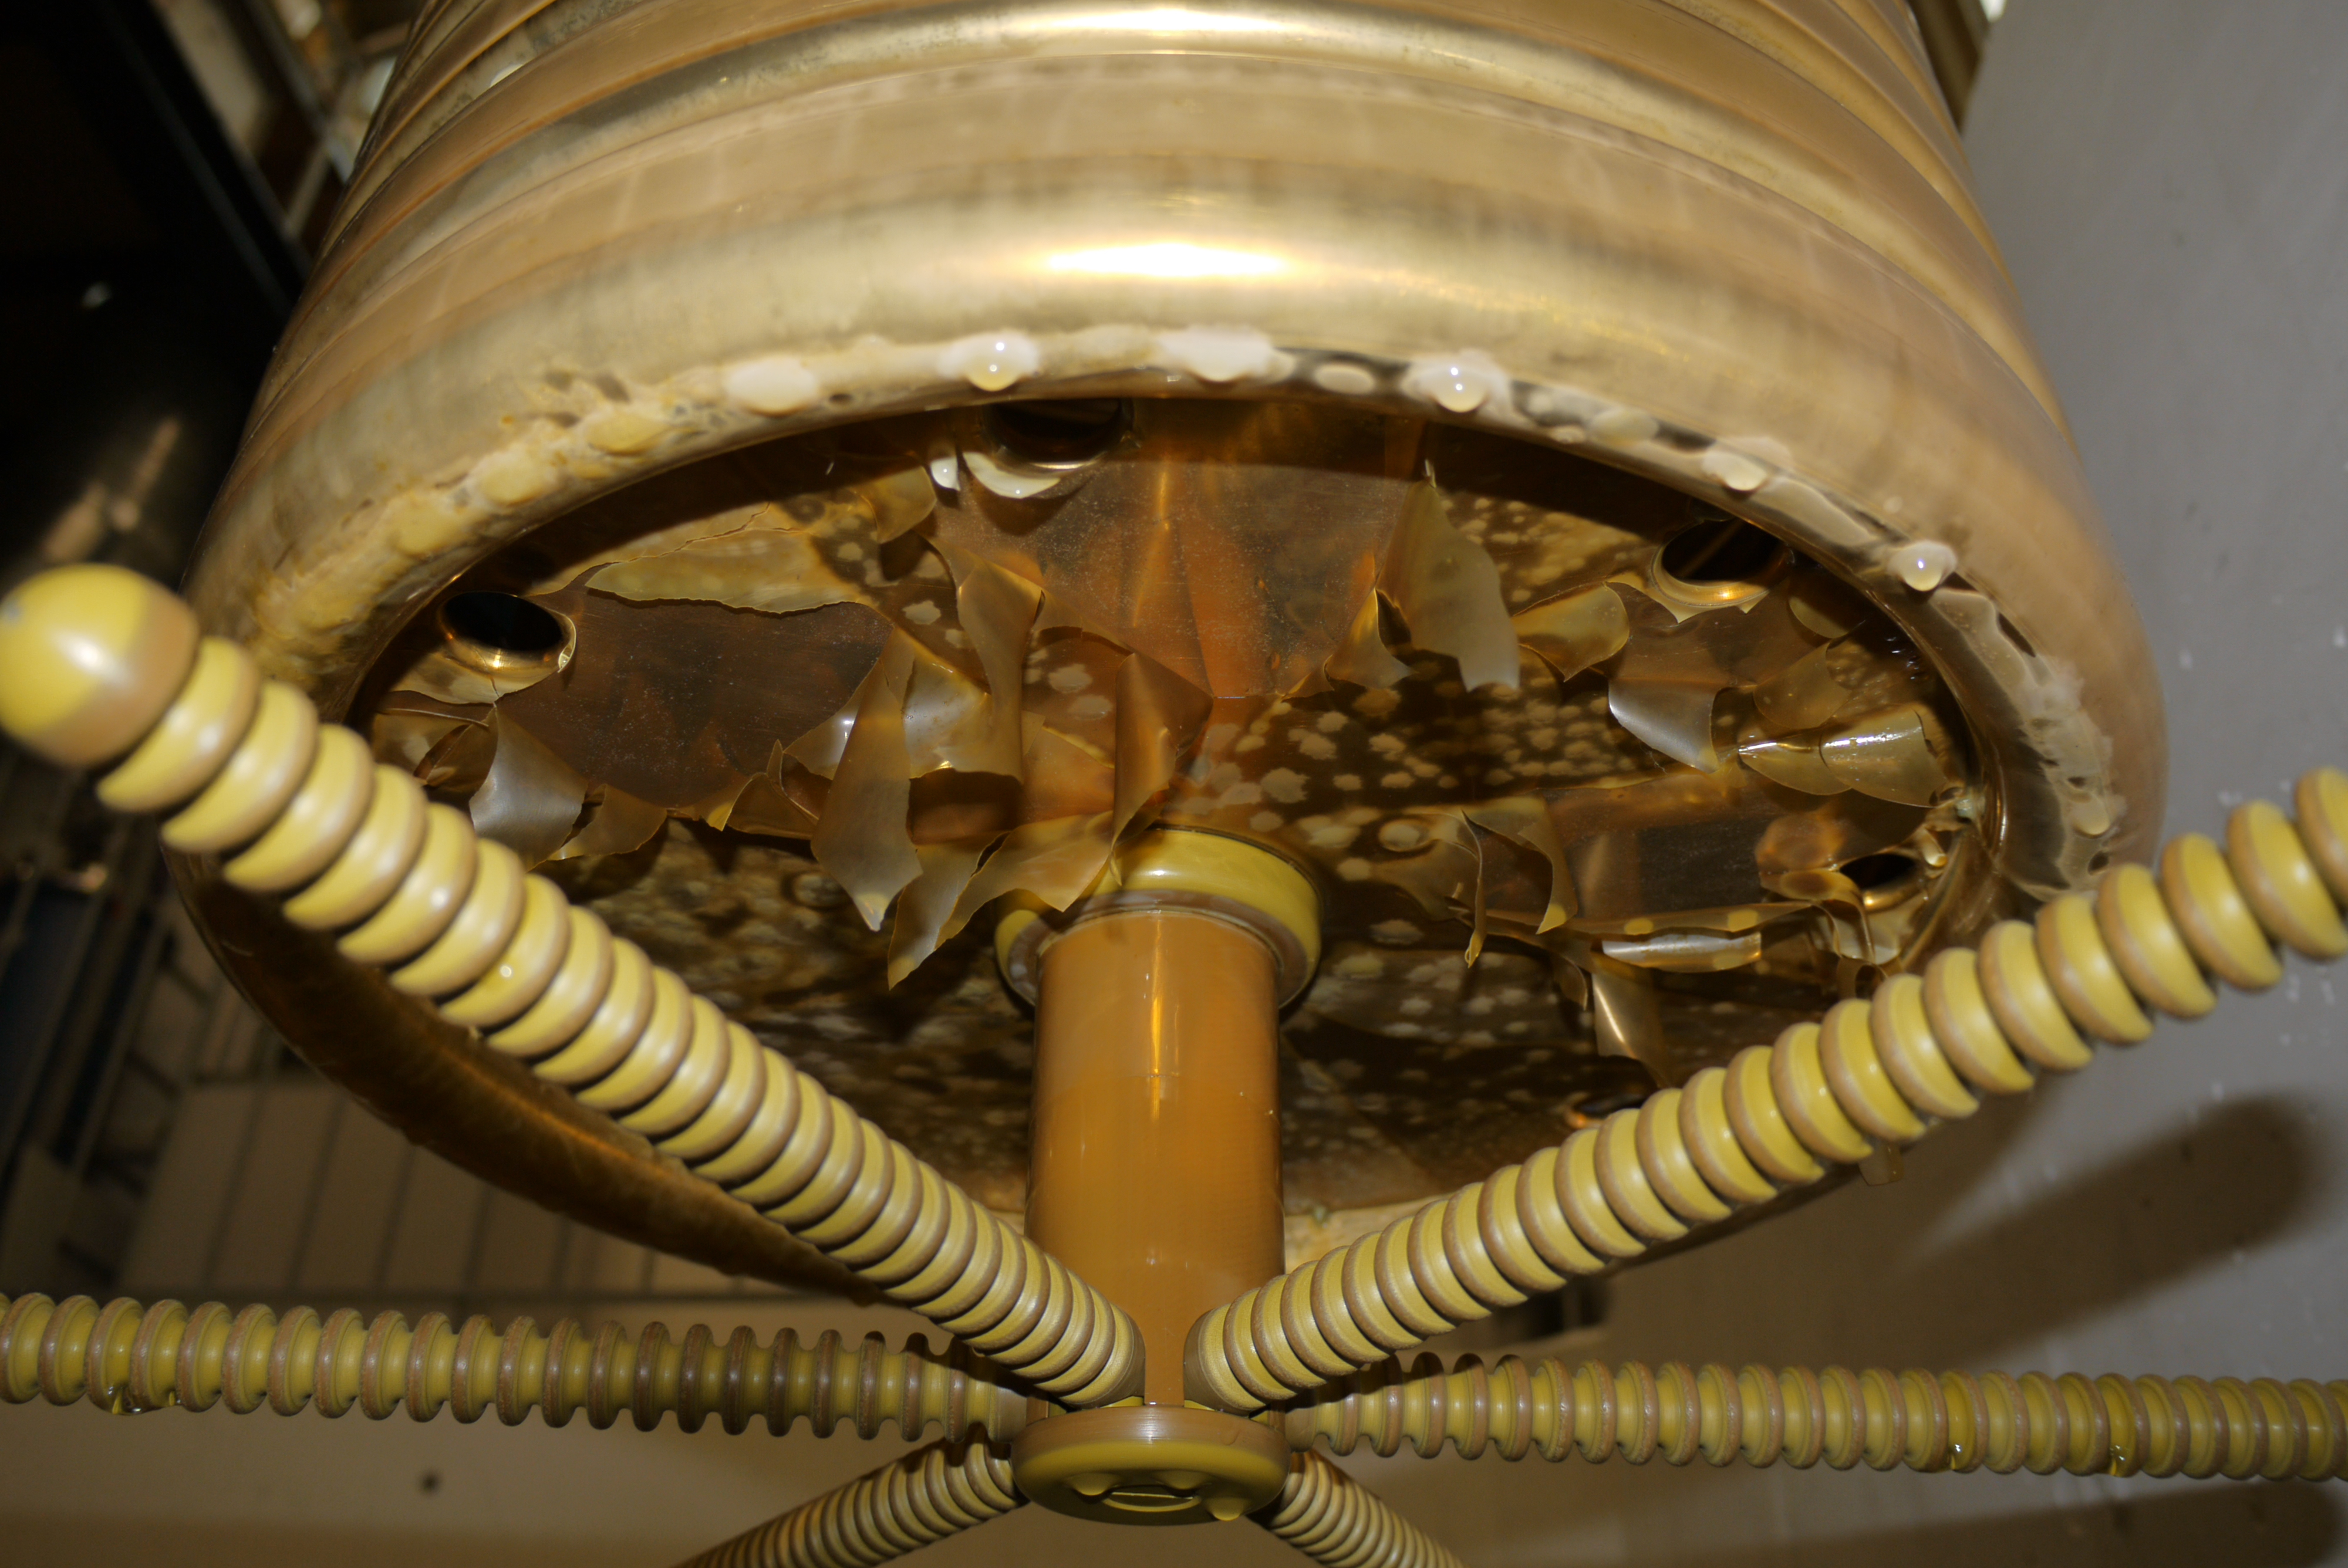
\includegraphics[height=.95\textwidth, angle=90]{defence/AT_cathode}
	\end{columns}
	\centering
	{\tiny Auger, Goeldi et al.\ arXiv:~1406.3929~\cite{latex}}\\
\end{frame}

\begin{frame}{Drift field generation summary}{\color{\emphcol} We need a modular TPC design}
	\begin{columns}[c]
		\column{.5\textwidth}
		\centering
		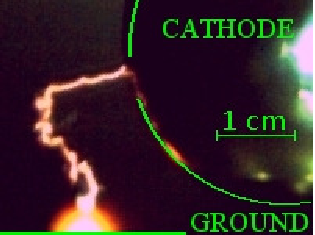
\includegraphics[width=\textwidth]{hv/sidespark}
		\column{.5\textwidth}
		\begin{itemize}
			\item Maximum safe electric field in \lar{}: \SI{40}{\kilo\volt\per\centi\metre}
			\item Can be increased by coating HV components
			\item Not practical (yet)
			\item[$\Rightarrow$] Large inactive clearance volumes around HV components
			\item[$\Rightarrow$] {\color{\emphcol} Segment TPC to keep cathode voltages low}
		\end{itemize}
	\end{columns}
\end{frame}

\section{Charge readout}

\begin{frame}{The standard \lartpc{} design}{Charge readout}
	\centering
	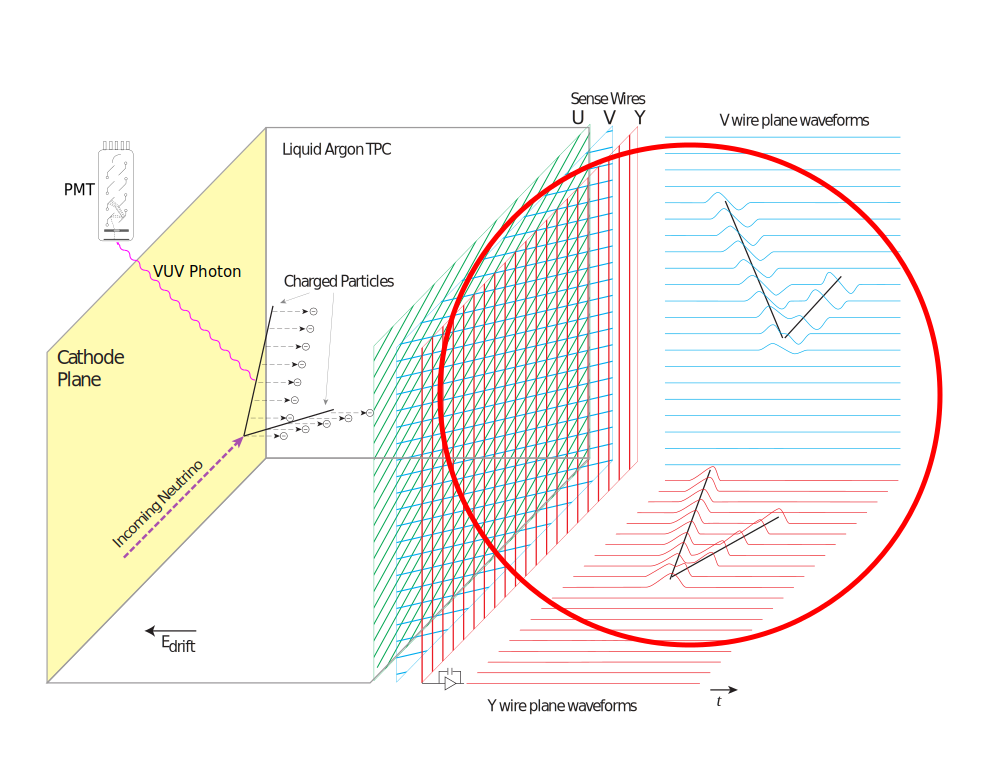
\includegraphics[viewport=35 40 755 540, clip, height=.66\textheight]{defence/TPCprinciple_charge-ro}\\
	{\tiny \uboone{} arXiv:~1612.05824~\cite{uboone}}\\
\end{frame}

\subsection{Wires}

\begin{frame}{Cosmic event}{\color{\emphcol} Effect of dead wires}
	\centering
	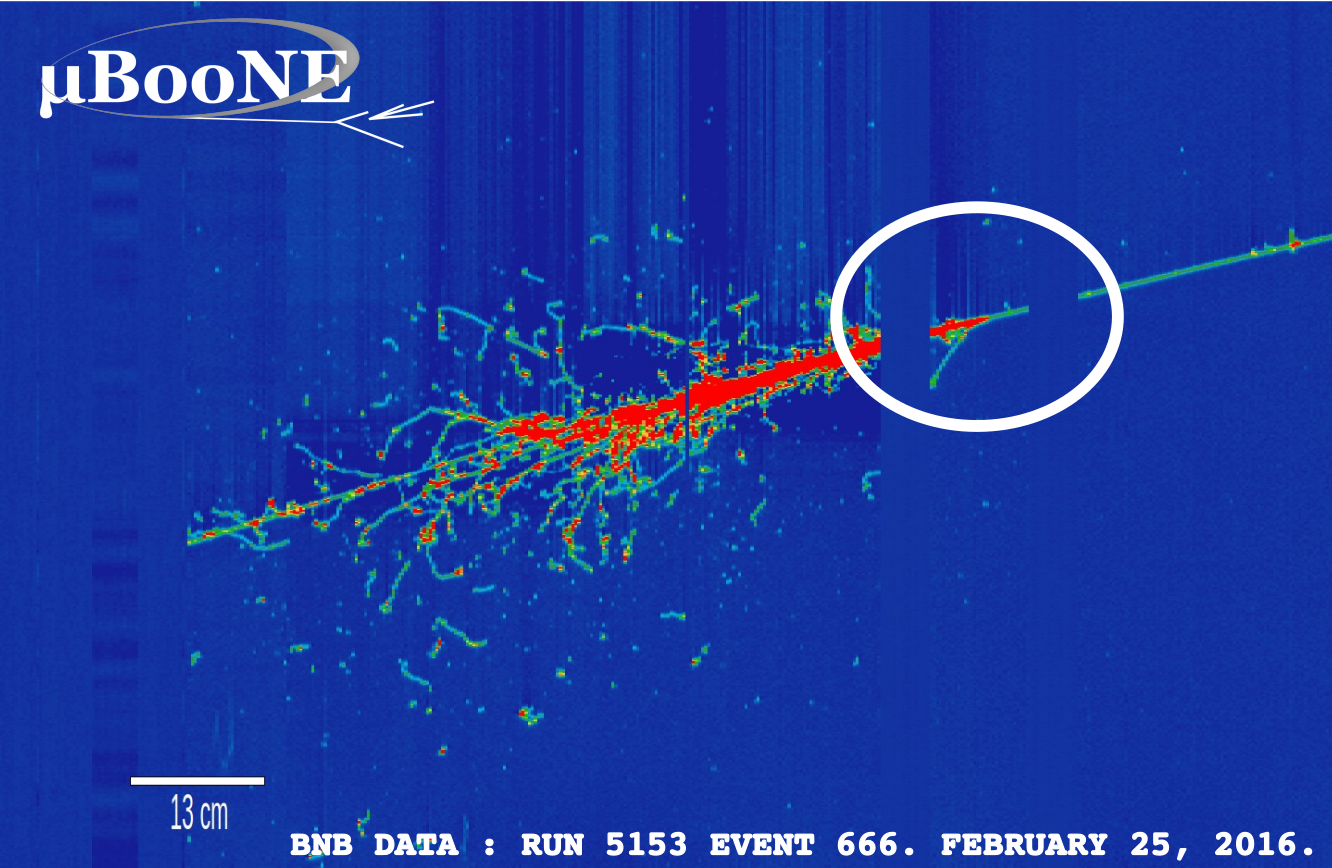
\includegraphics[height=.8\textheight]{defence/uboone_em-shower_dead-wires}
\end{frame}

\begin{frame}{Problems of wire readouts}
	\begin{columns}[c]
		\column{.4\textwidth}
		\centering
		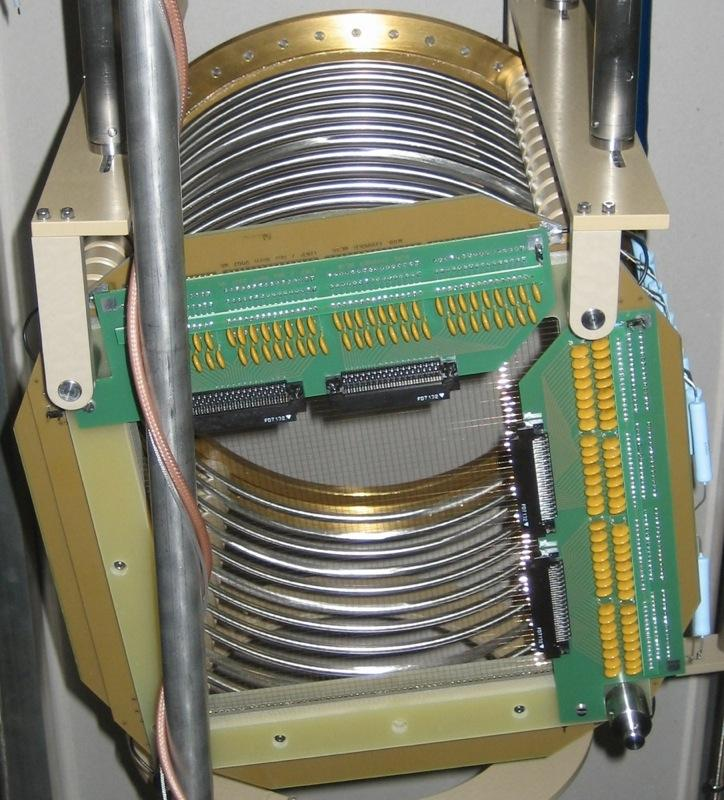
\includegraphics[width=\textwidth]{defence/mat_wires}\\
		{\tiny University of Bern, 2009}\\
		\column{.6\textwidth}
		For decades, sensing wires have done a great job
		BUT they have many drawbacks:
		\begin{itemize}
			\item Only 2D projections of 3D event (either XZ, YZ or UZ, VZ, WZ)
			\item Ambiguities in reconstruction
			\item Mechanically highly demanding (design \& production)
			\item Prone to microphonics
		\end{itemize}
		{\color{\emphcol} Reducing an ideal 3D tracker to multiple 2D projections}
	\end{columns}
\end{frame}

\subsection{Pixels}

\begin{frame}{Why (not) pixels?}
	\begin{columns}[c]
		\column{.5\textwidth}
		\centering
		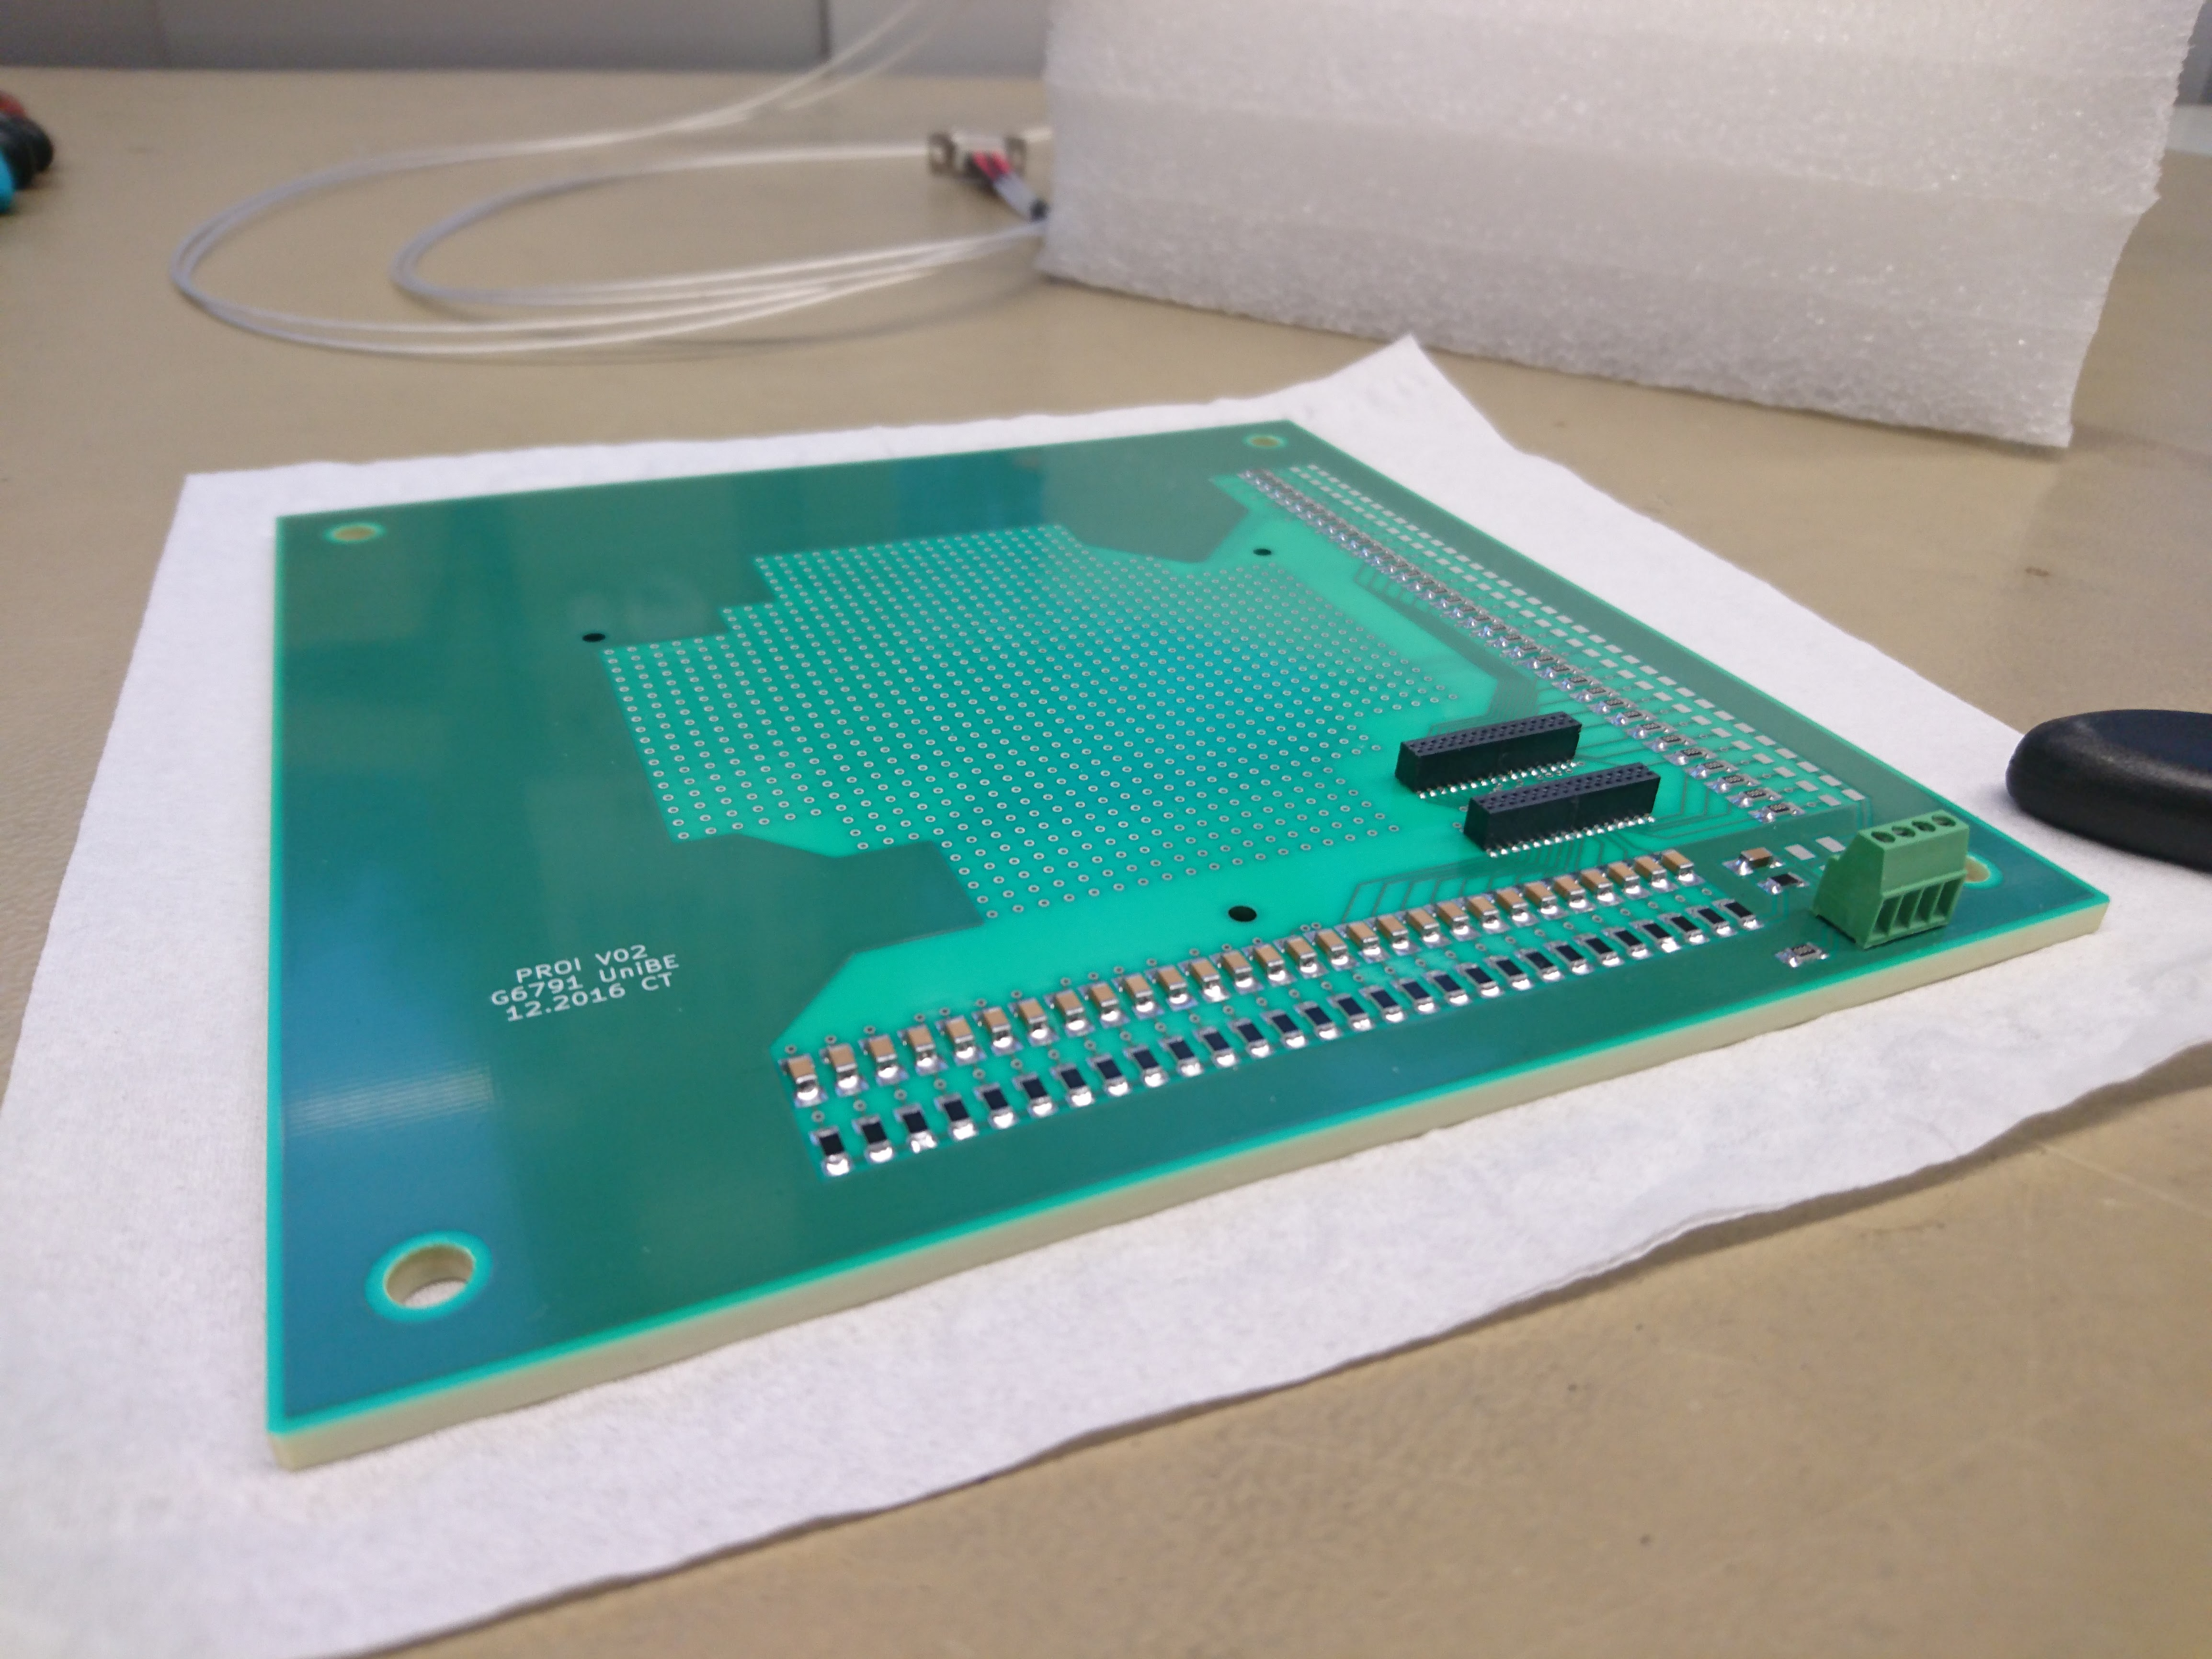
\includegraphics[width=\textwidth]{defence/pcb_new}\\
		{\tiny University of Bern, 2017}\\
		\column{.5\textwidth}
		\begin{itemize}
			\item Complete 3D event reconstruction w/o ambiguities
			\item {\color{\emphcol} Roughly squared number of readout channels}
			\item E.g.\ \uboone{}:
			\begin{itemize}
				\item \SI{10 x 2}{\metre}
				\item $\order{\num{e4}}$~wires
				\item[$\rightarrow$] $\order{\num{e7}}$~pixels
			\end{itemize}
			\item Extremely high number of cryostat penetrations
		\end{itemize}
	\end{columns}
\end{frame}

\begin{frame}{Handling high channel numbers}
	\begin{columns}[c]
		\column{.5\textwidth}
		\centering
		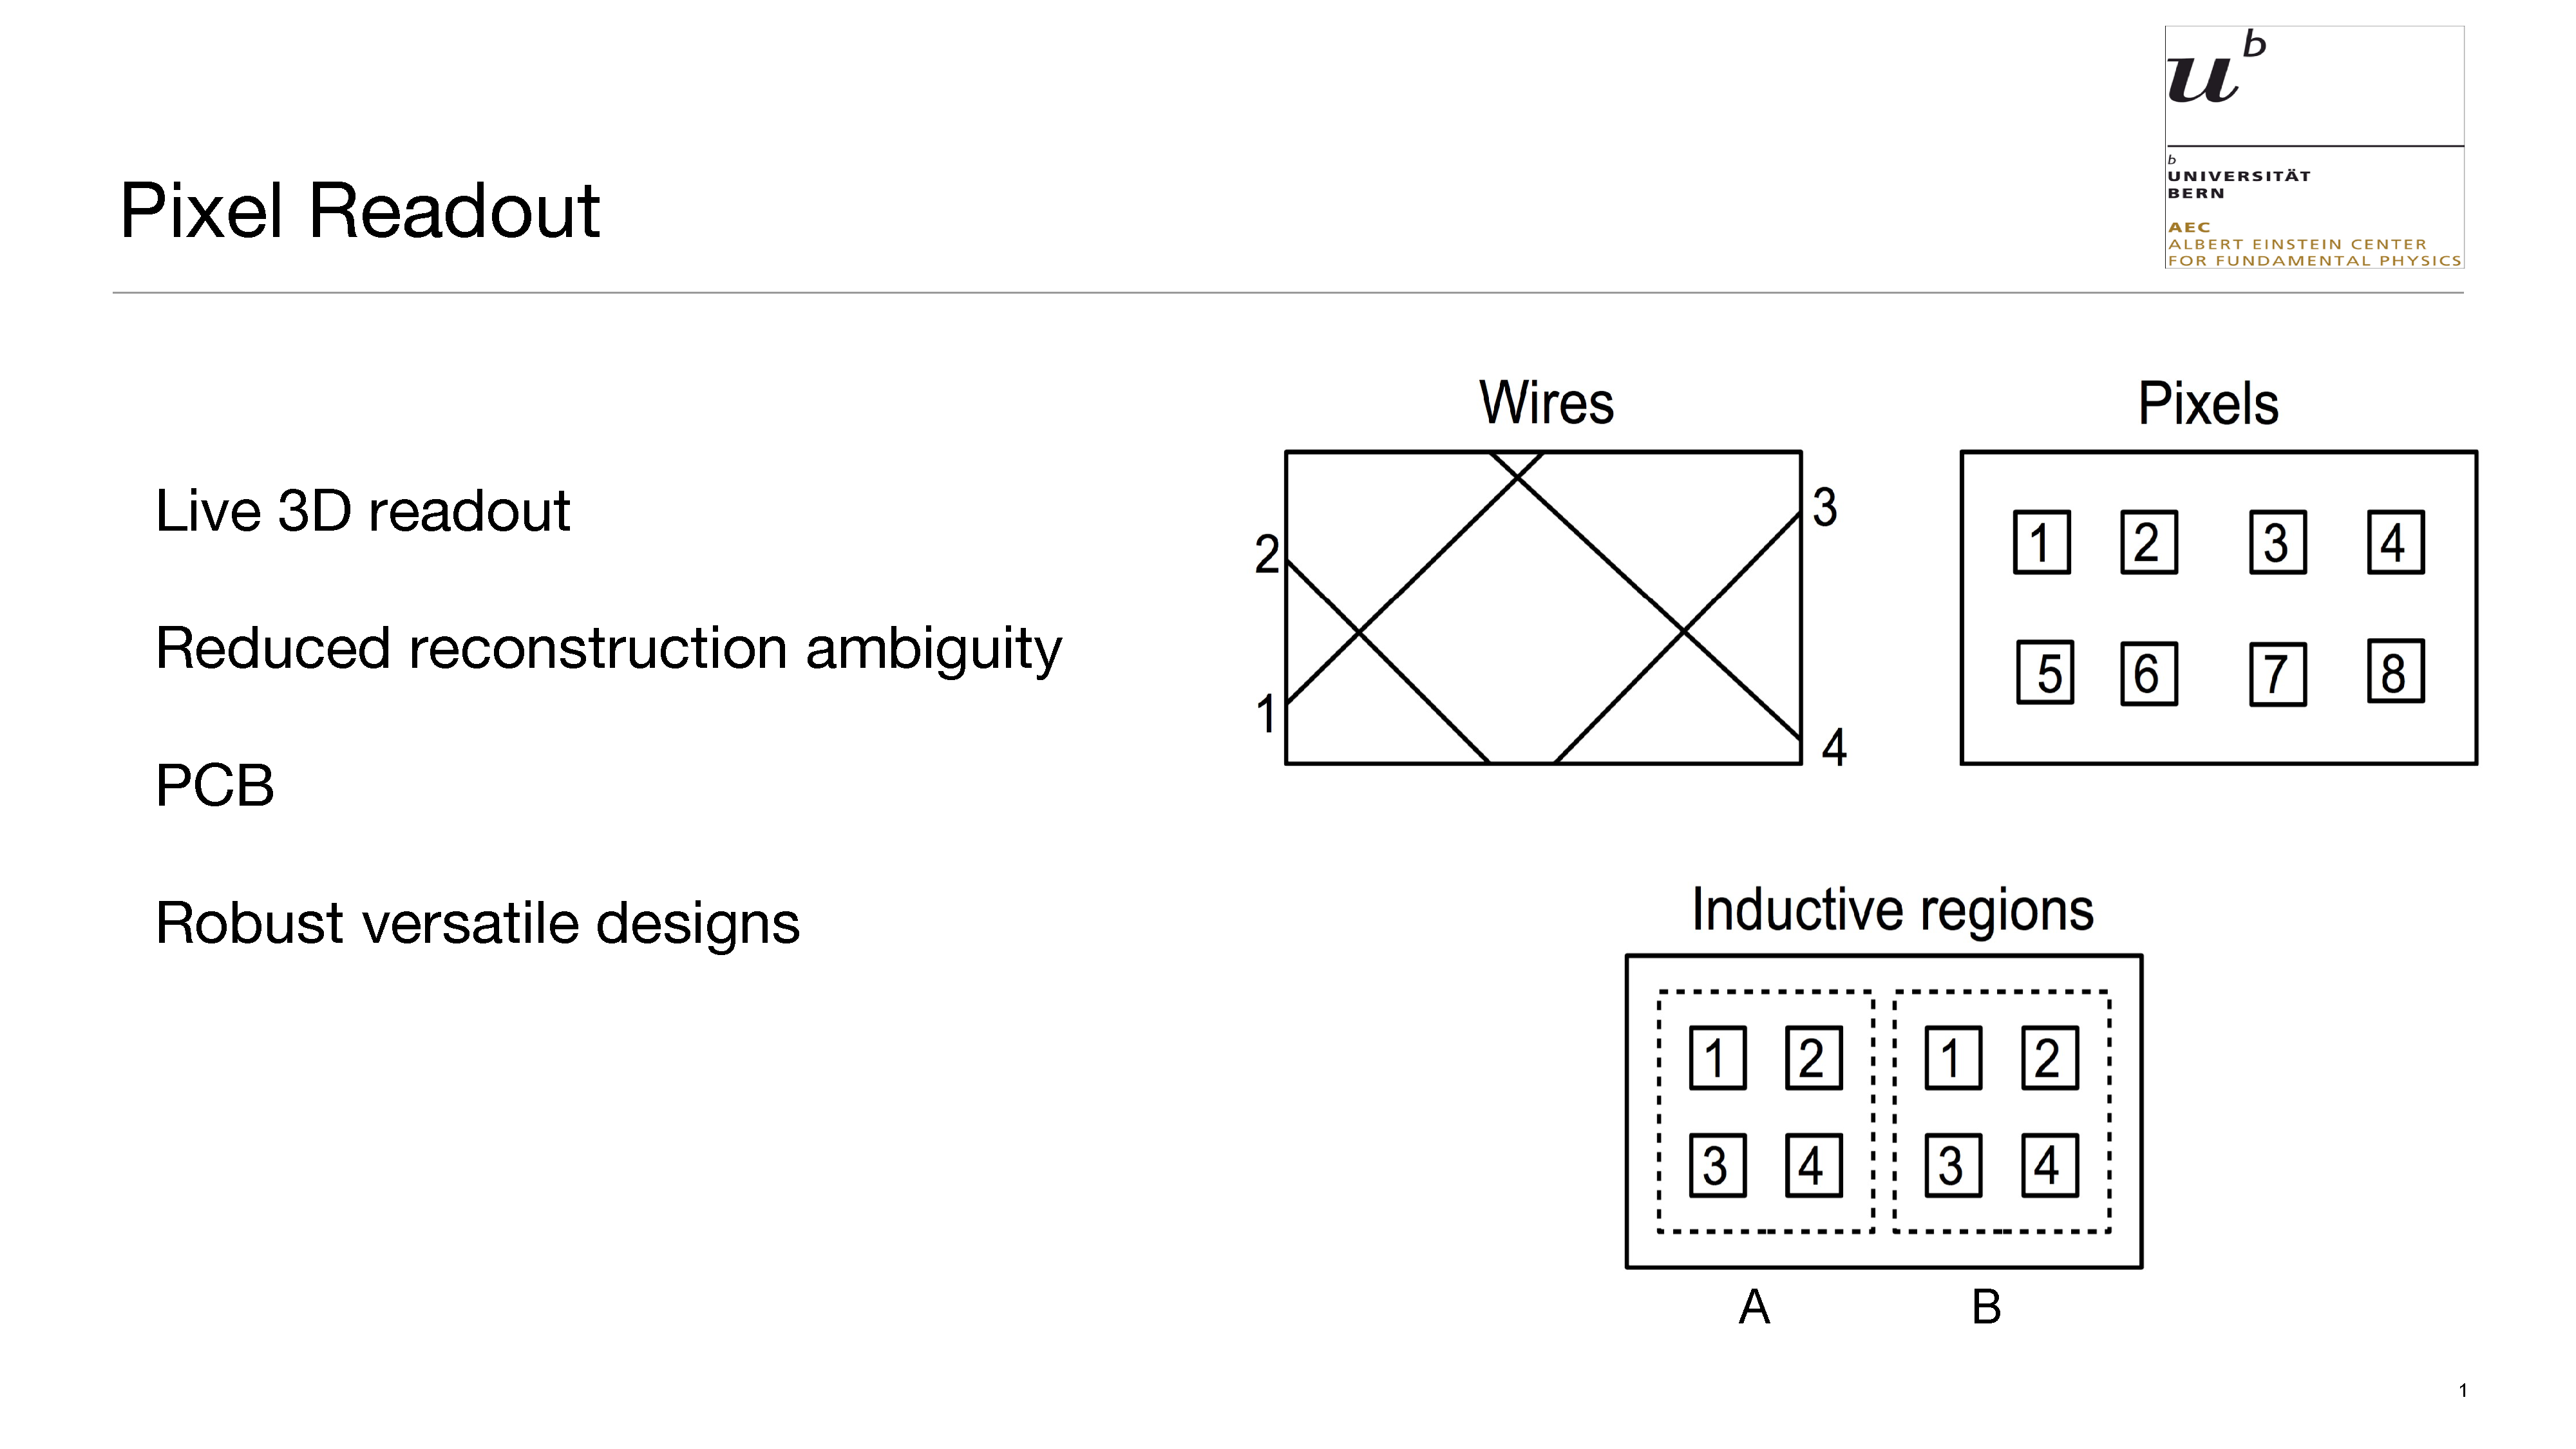
\includegraphics[page=1, viewport=930 90 1850 800, clip, width=\textwidth]{defence/Pixels}\\
		Multiplexing
		\column{.5\textwidth}
		\begin{itemize}
			\item Cold digitisation
			\begin{itemize}
				\item[$+$] high-speed digital links
				\item[$+$] potentially less noise
				\item[$-$] complex cold electronics
				\item[$-$] high power dissipation
			\end{itemize}
			\item {\color{\emphcol} Analogue multiplexing}
			\begin{itemize}
				\item[$+$] existing cold electronics
				\item[$-$] ambiguities
			\end{itemize}
		\end{itemize}
	\end{columns}
\end{frame}

\subsection{\AC\ pixel demonstrator}

\begin{frame}{\AC\ pixel demonstrator PCB}{\num{28} ROIs, each \num{6 x 6} pixels $\Rightarrow$ {\color{\emphcol} \num{64} DAQ channels $\rightarrow$ \num{1008} physical pixels} @ \SI{2.54}{\milli\meter} pitch}
	\centering
	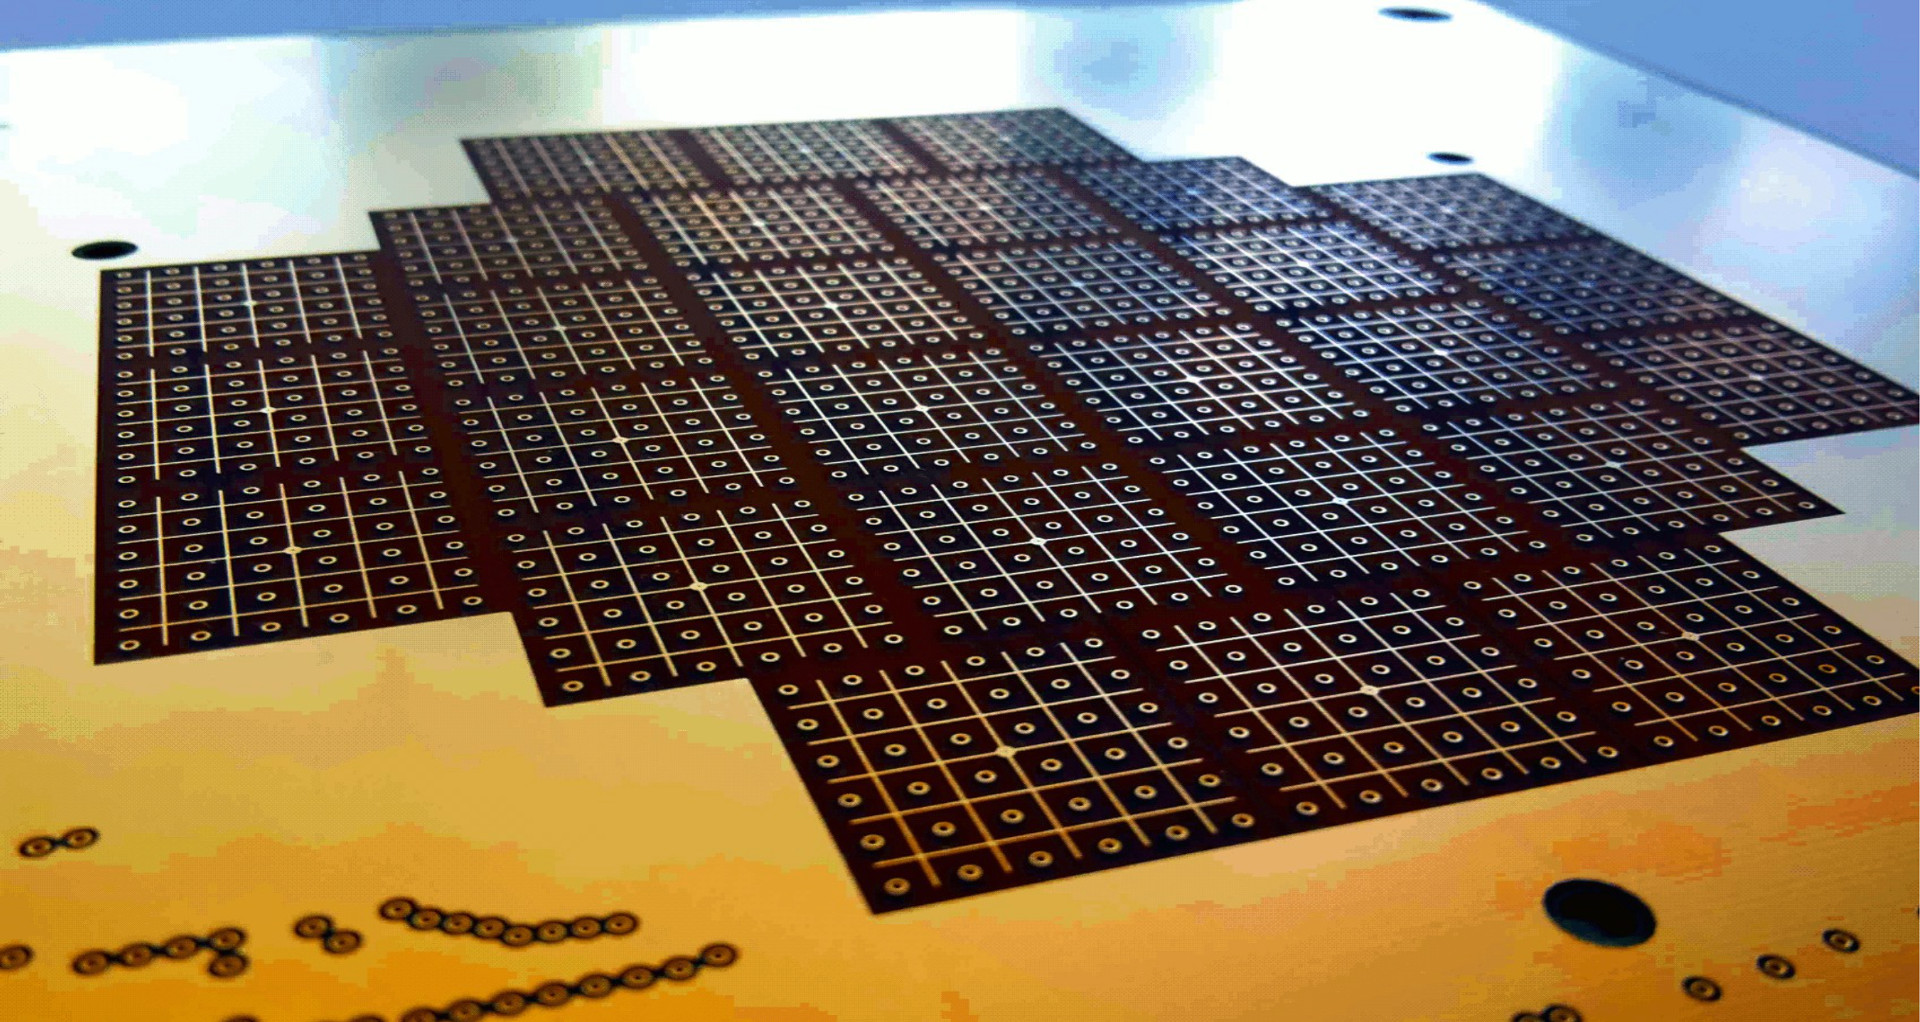
\includegraphics[width=\textwidth]{viper/pixies}
\end{frame}

\begin{frame}{\AC\ pixel demonstrator TPC}
	\begin{columns}[c]
		\column{.5\textwidth}
		\centering
		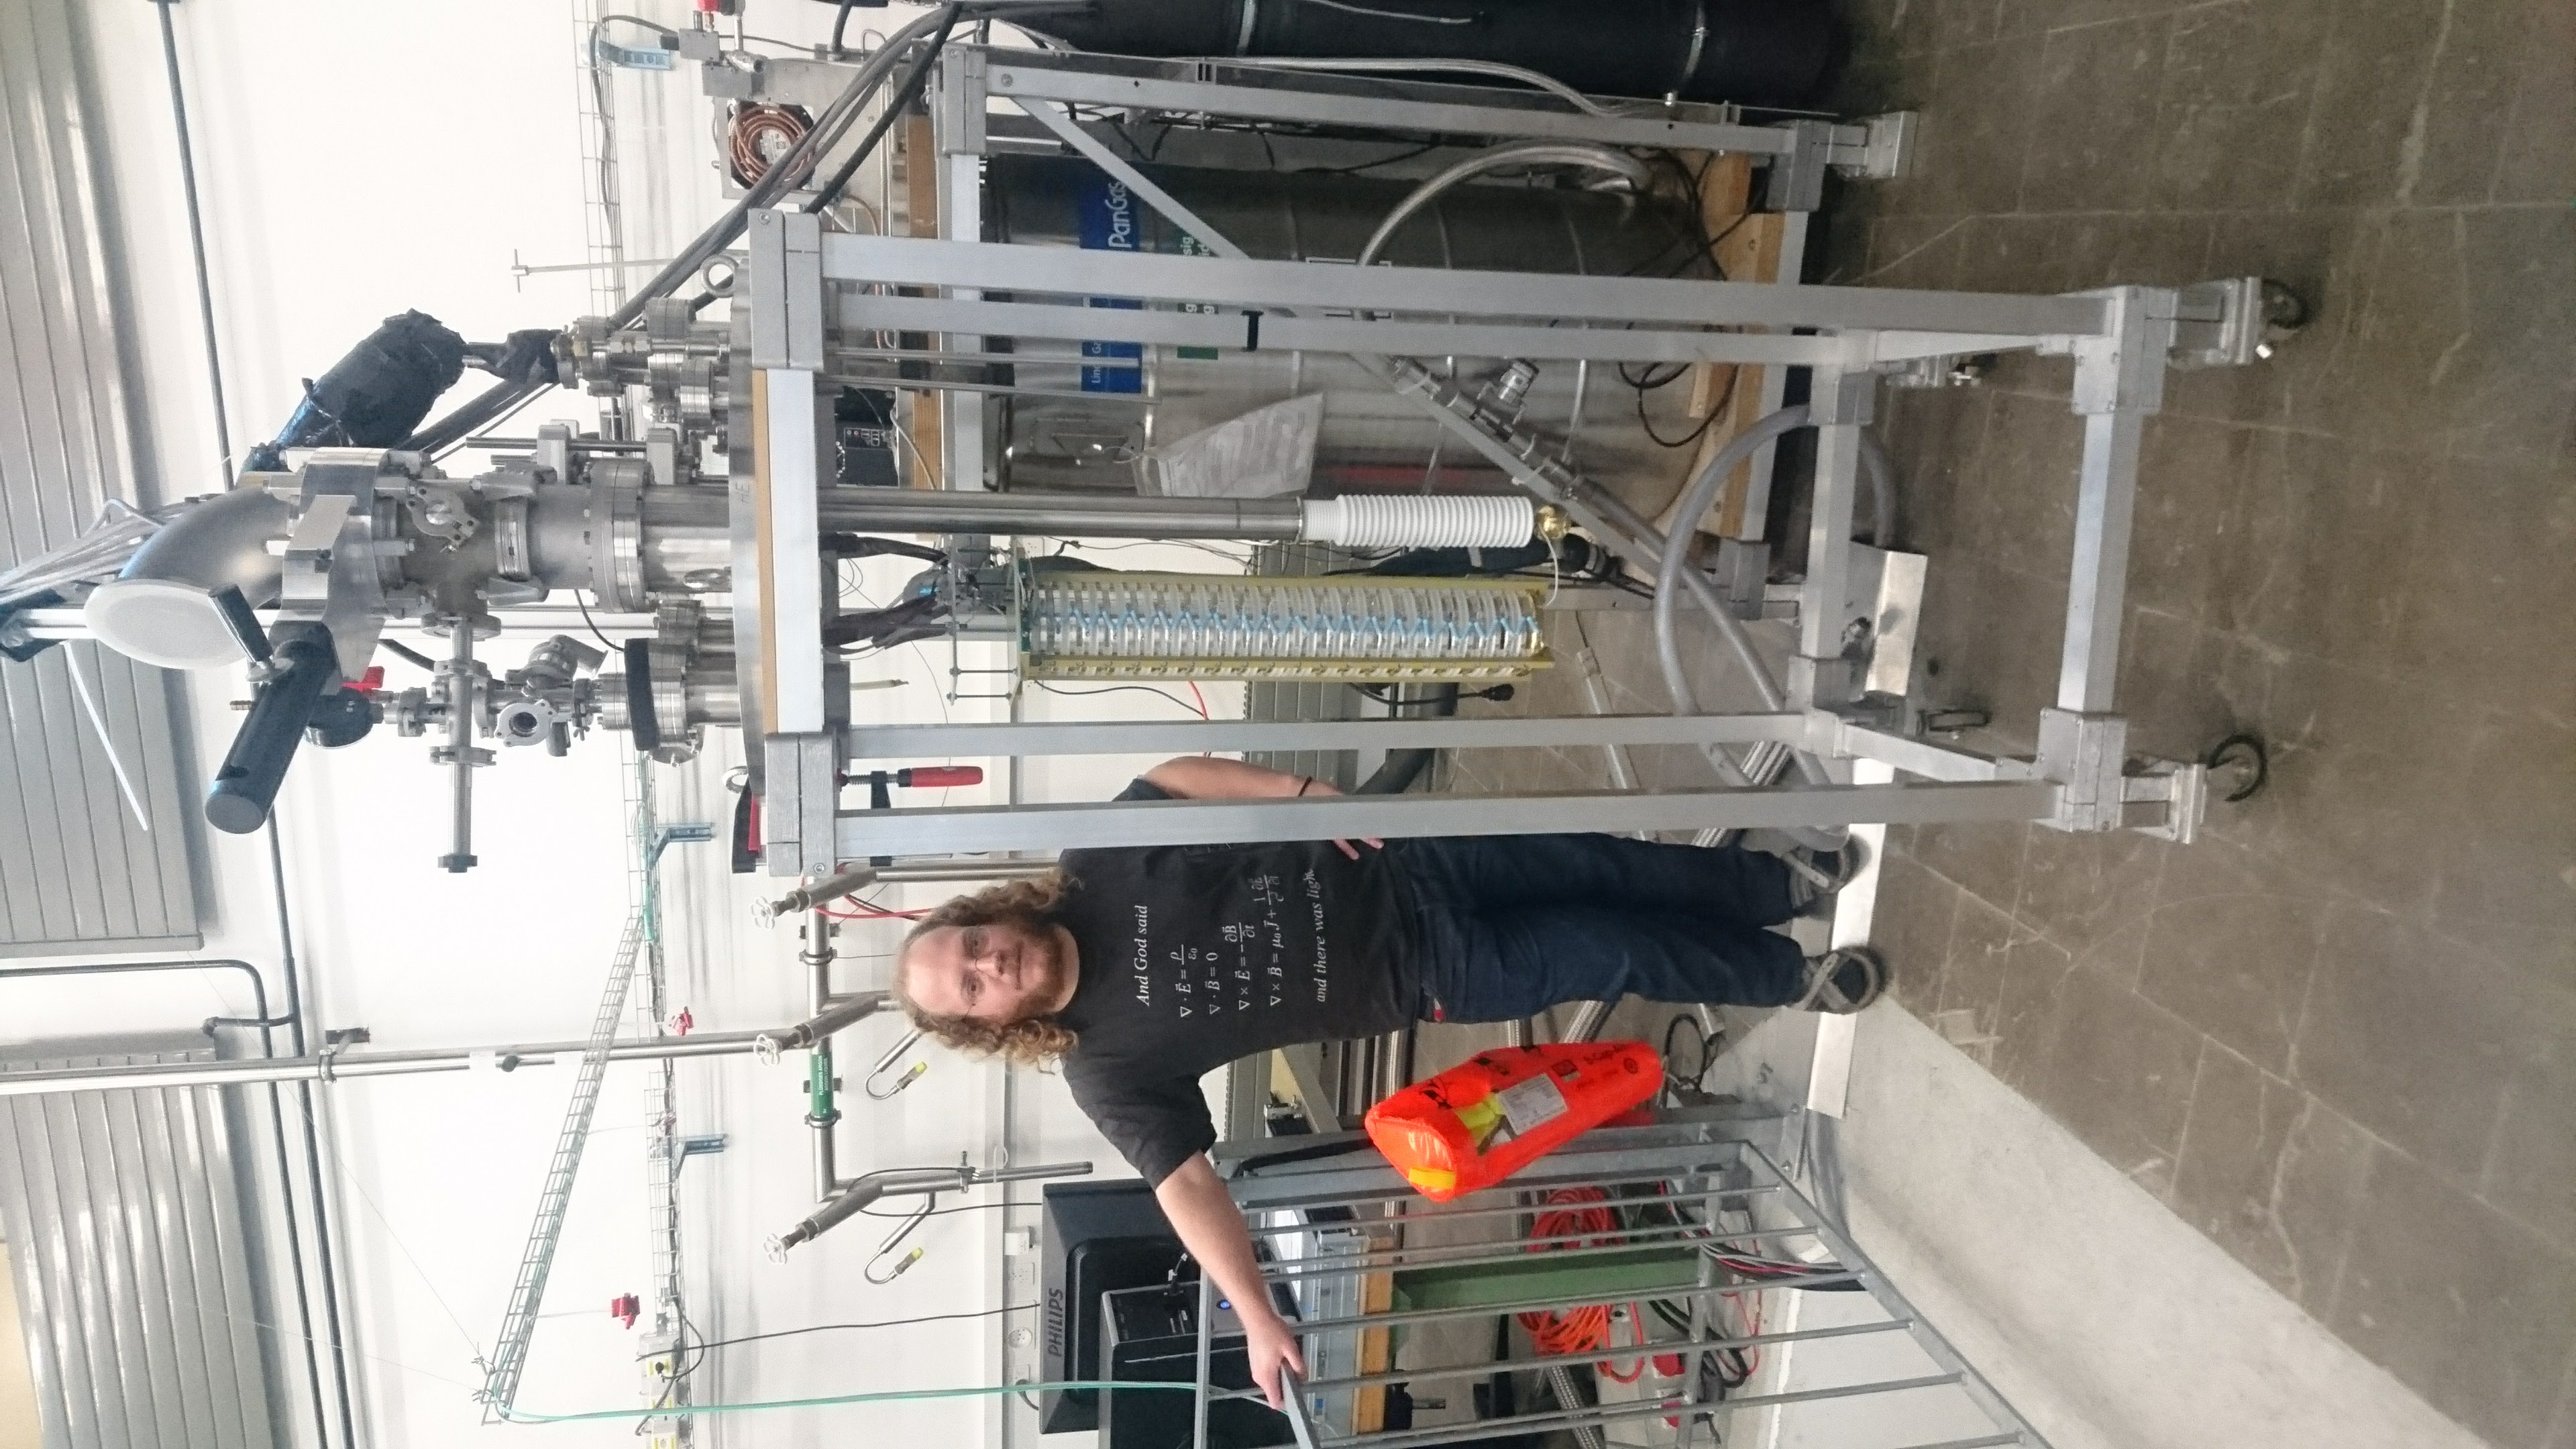
\includegraphics[viewport=1200 200 2500 1800, clip, height=\textwidth, angle=-90]{defence/TPC}\\
		{\tiny University of Bern, 2017}\\
		\column{.5\textwidth}
		\begin{itemize}
			\item \SI{200}{\litre} bath cryostat, $\varnothing = \SI{500}{\milli\meter}$, $h = \SI{1100}{\milli\metre}$
			\item \SI{130}{\kilo\volt} HV feedthrough
			\item Cylindrical drift volume
			\item $\varnothing = \SI{100}{\milli\meter}$
			\item $L = \SI{600}{\milli\meter}$
			\item $V_{\m{Drift}} = \SI{60}{\kilo\volt}$
			\item[$\Rightarrow$] {\color{\emphcol} $E_{\m{Drift}} = \SI{0.1}{\kilo\volt\per\milli\meter}$}
			\item[$\Rightarrow$] $v_{\m{Drift}} = \SI{2}{\milli\meter\per\micro\second}$
			\item[$\Rightarrow$] {\color{\emphcol} $t_{\m{Drift}} = \SI{300}{\micro\second}$}
		\end{itemize}
	\end{columns}
\end{frame}

\begin{frame}{\AC\ pixel demonstrator readout}
	\begin{columns}[c]
		\column{.5\textwidth}
		\centering
		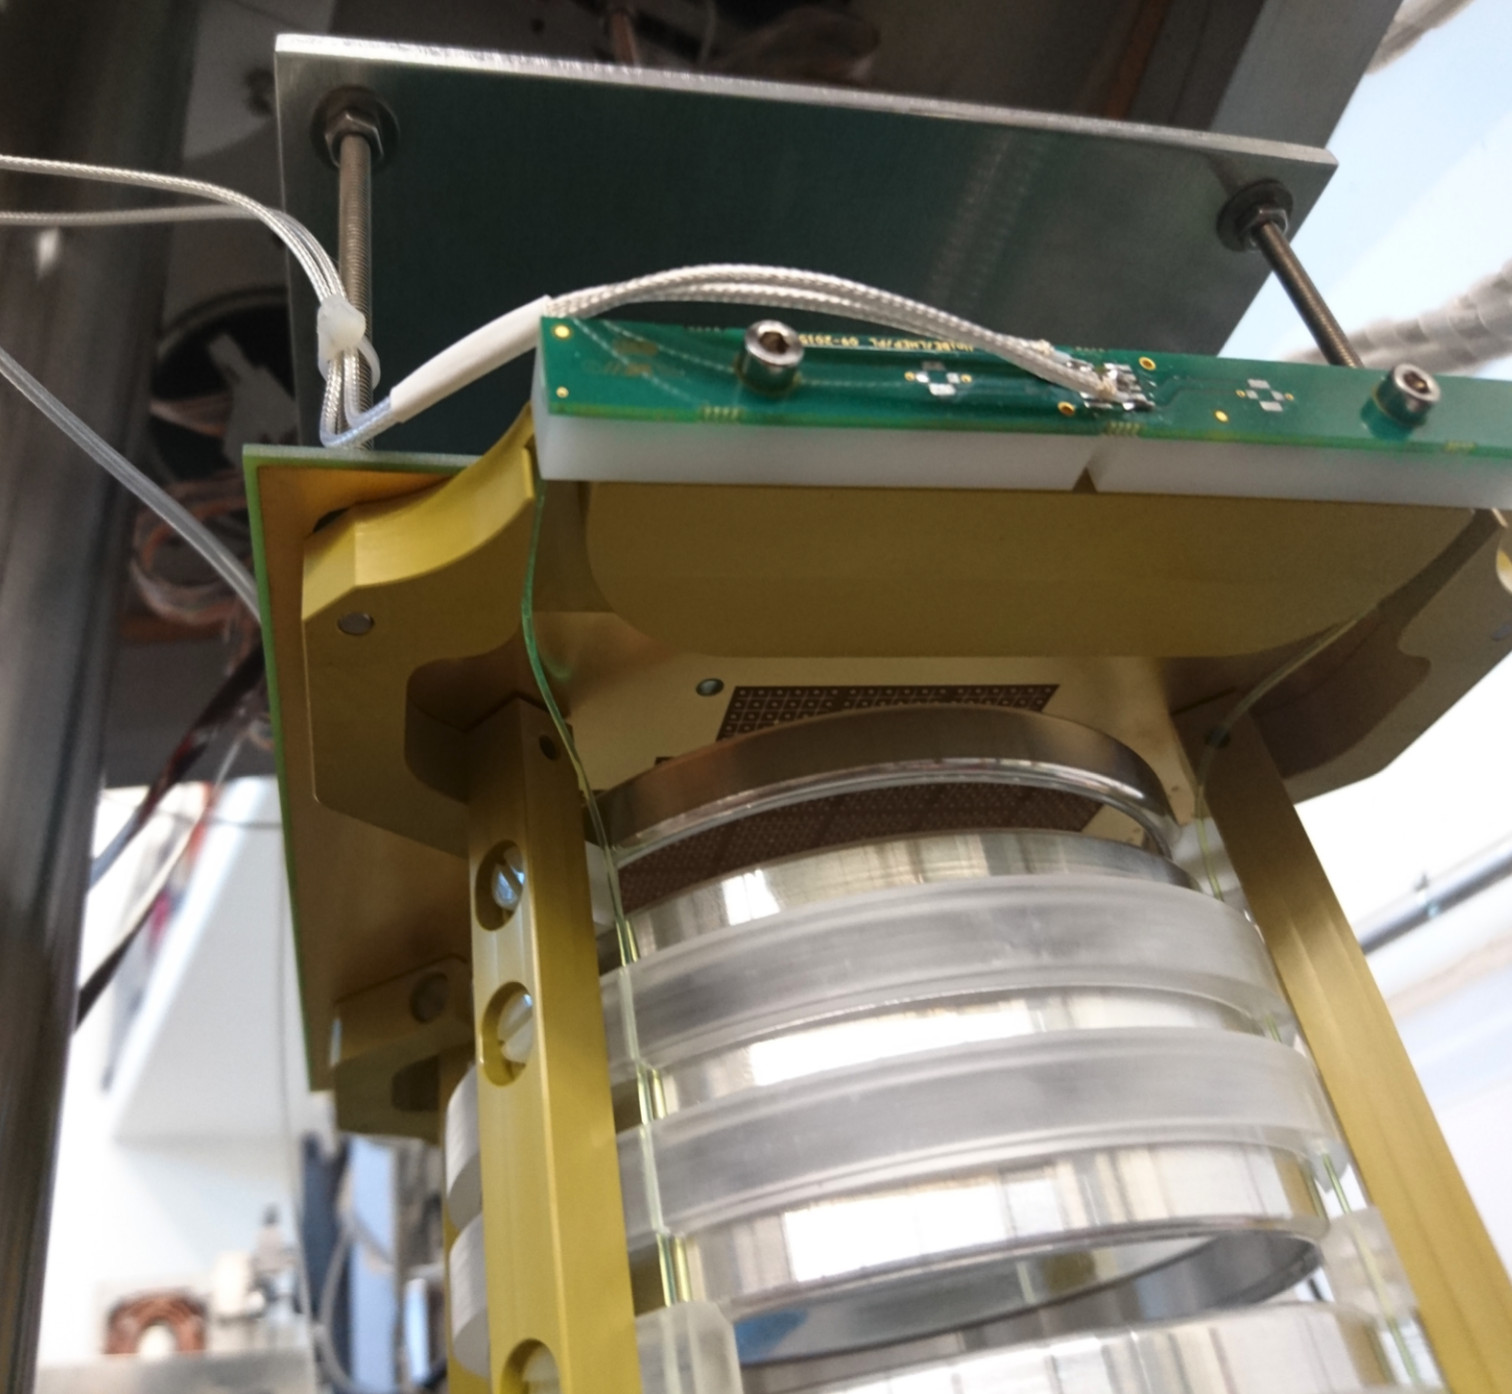
\includegraphics[width=\textwidth]{viper/viper_sipm}\\
		{\tiny University of Bern, 2017}\\
		\column{.5\textwidth}
		\begin{itemize}
			\item \num{64} DAQ channels for \num{1008} physical pixels
			\item {\color{\emphcol} Charge readout by BNL LARASIC4* preamplifiers in LAr}
			\item[$\hookrightarrow$] CAEN ADCs at room temperature
			\item Light readout by TPB coated acrylic field cage spacers (inner surface)
			\item[$\hookrightarrow$] {\color{\emphcol} Hamamatsu S12825-050P SiPMs in LAr}
		\end{itemize}
	\end{columns}
\end{frame}

\subsection{3D event reconstruction}

\begin{frame}{Regions of interest (ROI) multiplexing}
	\centering
	\includegraphics[page=2, viewport=20 0 1770 845, clip, width=\textwidth]{defence/Pixels}\\
	{\tiny James Sinclair, University of Bern}\\
\end{frame}

\begin{frame}{Raw charge data}
	\centering
	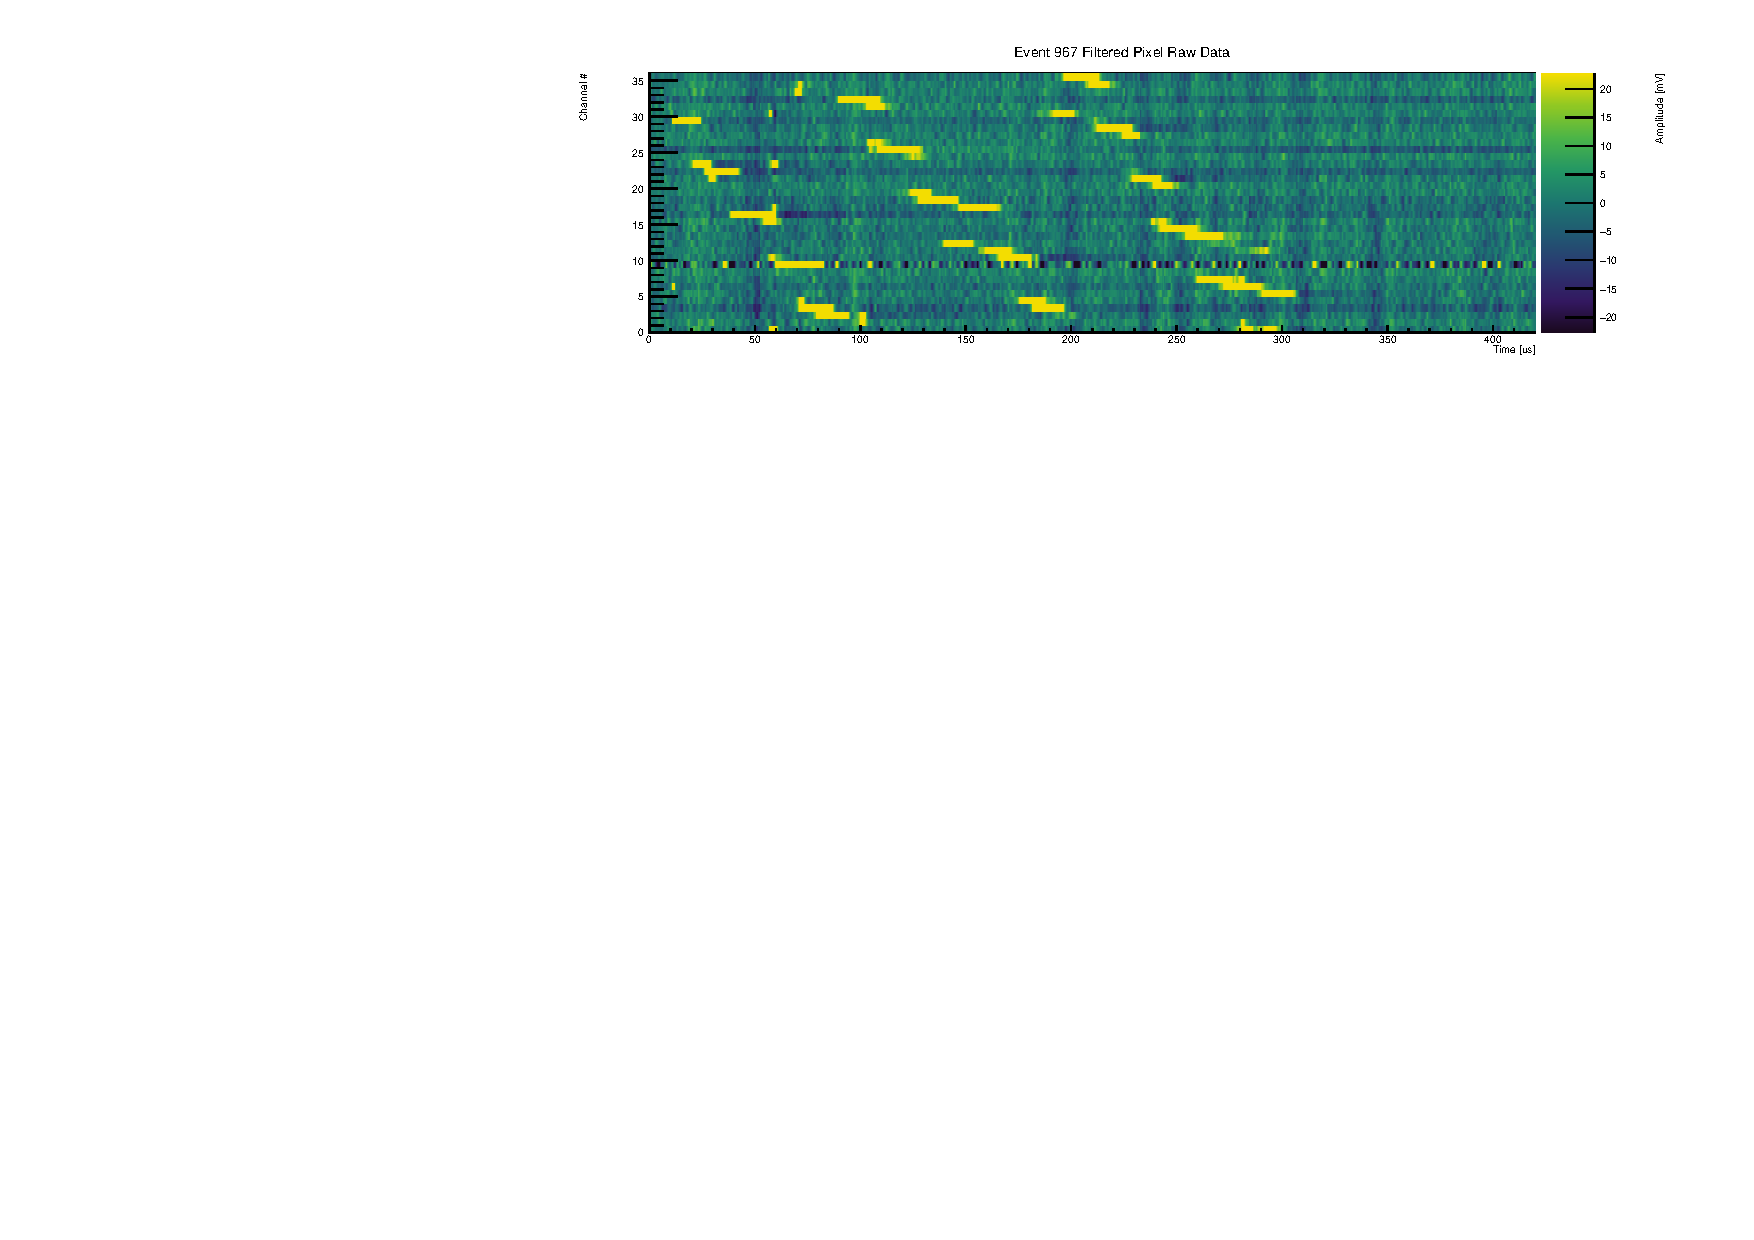
\includegraphics[width=\textwidth]{defence/event967_rawFilteredPixel}\\
	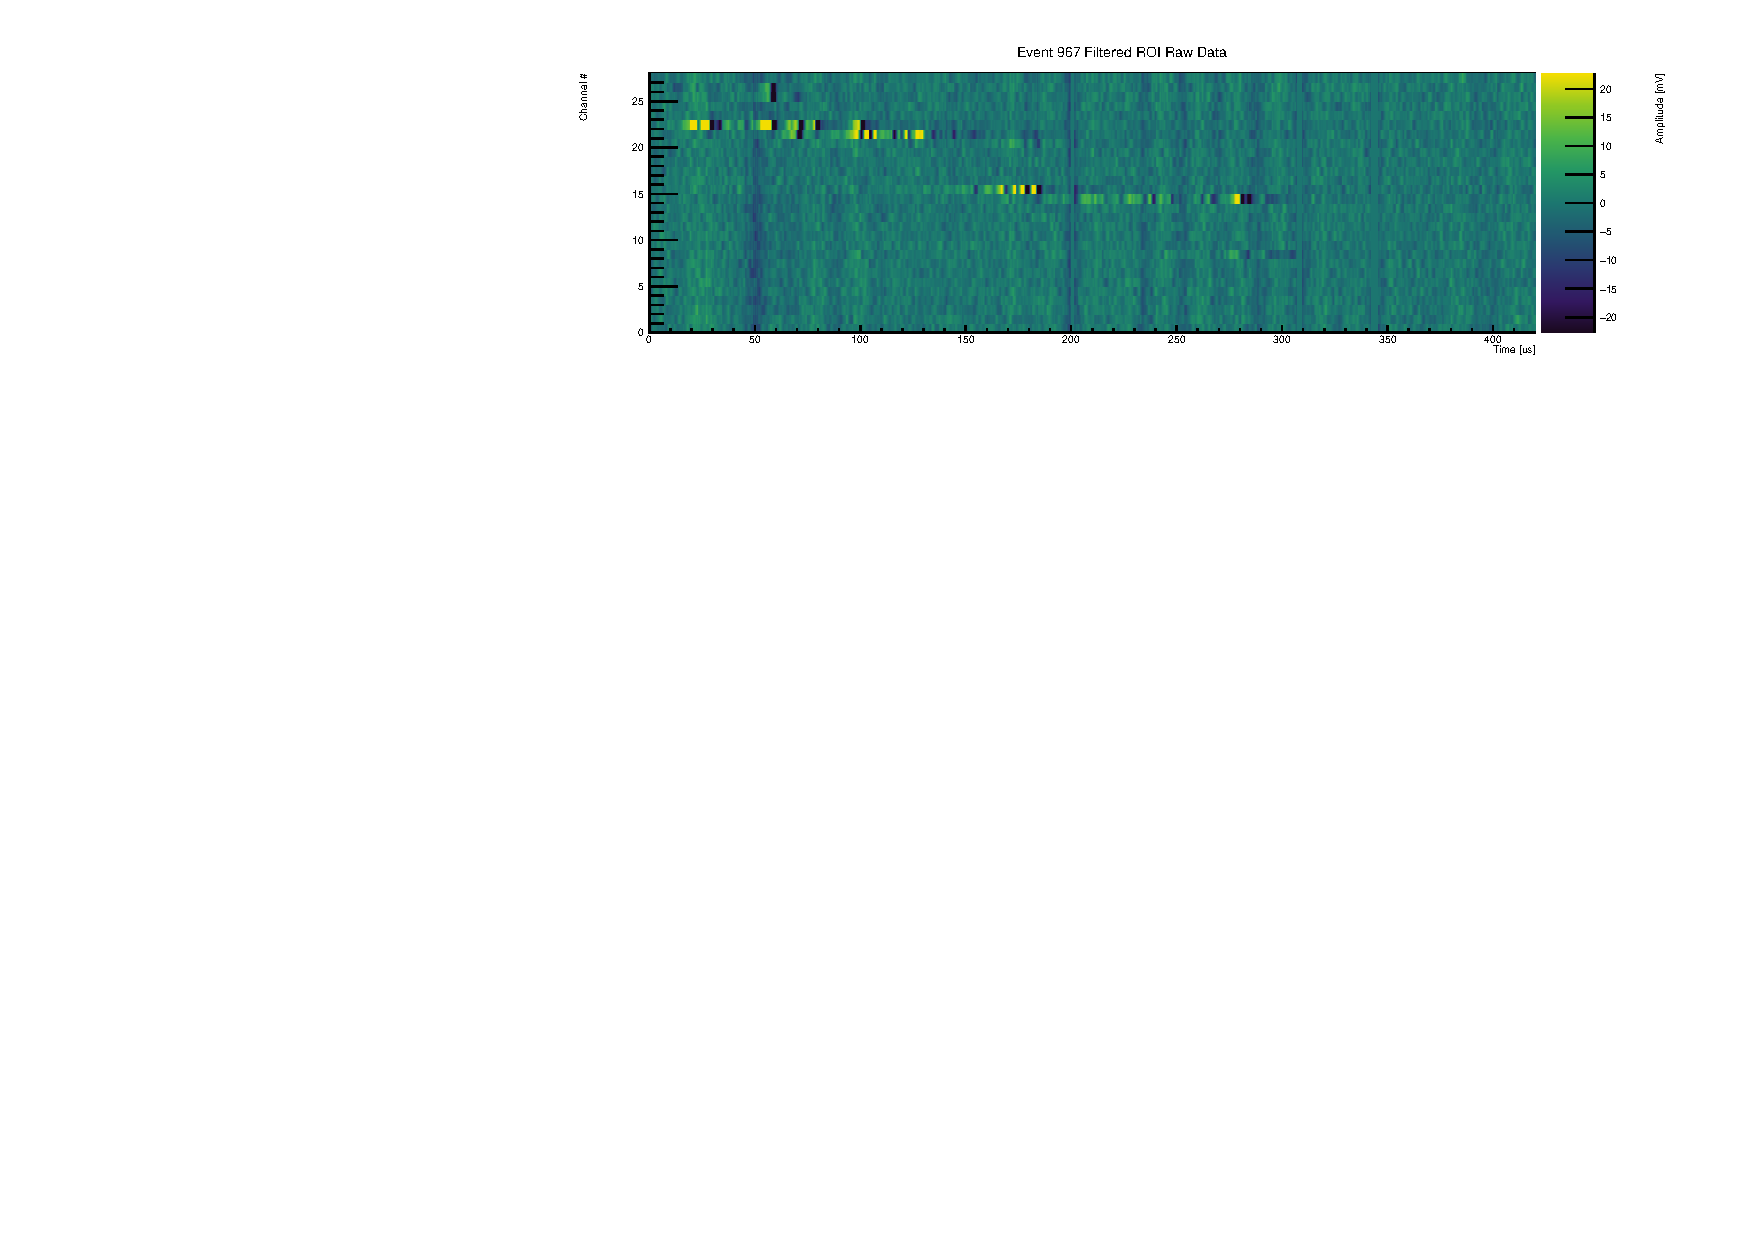
\includegraphics[width=\textwidth]{defence/event967_rawFilteredROI}\\
	{\tiny University of Bern, 2017}\\
\end{frame}

\begin{frame}{Reconstructed 3D event}
	\begin{columns}[c]
		\column{.4\textwidth}
		\centering
		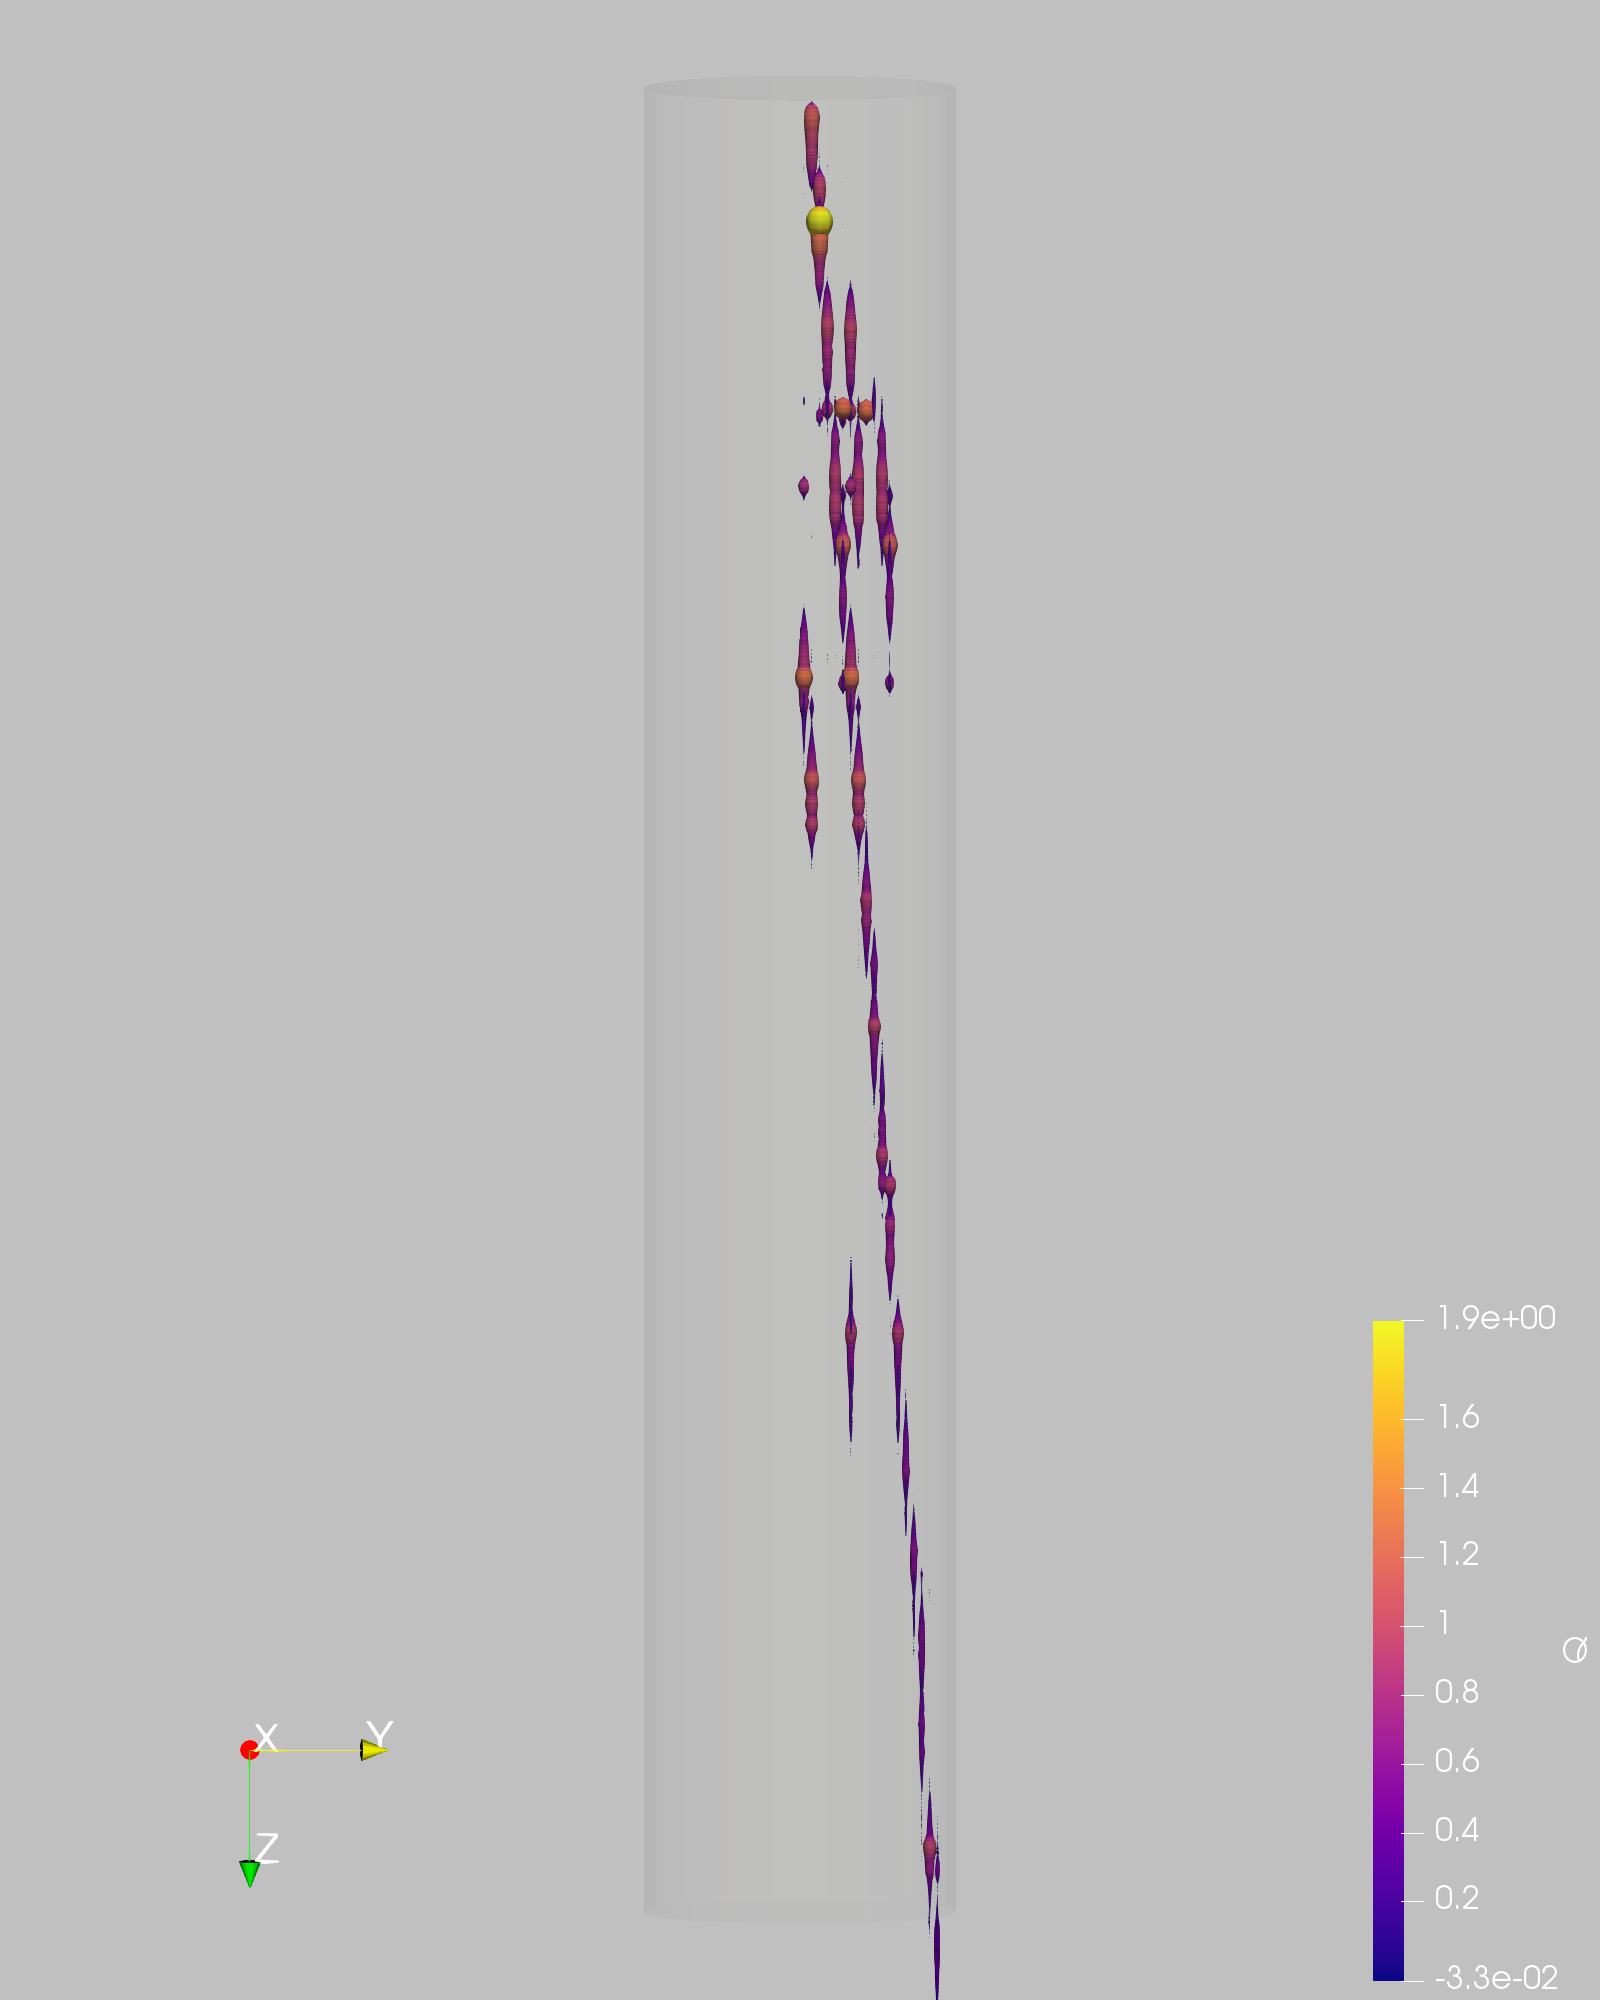
\includegraphics[width=\textwidth]{viper/event967_pulses_q}
		\column{.2\textwidth}
		\centering
		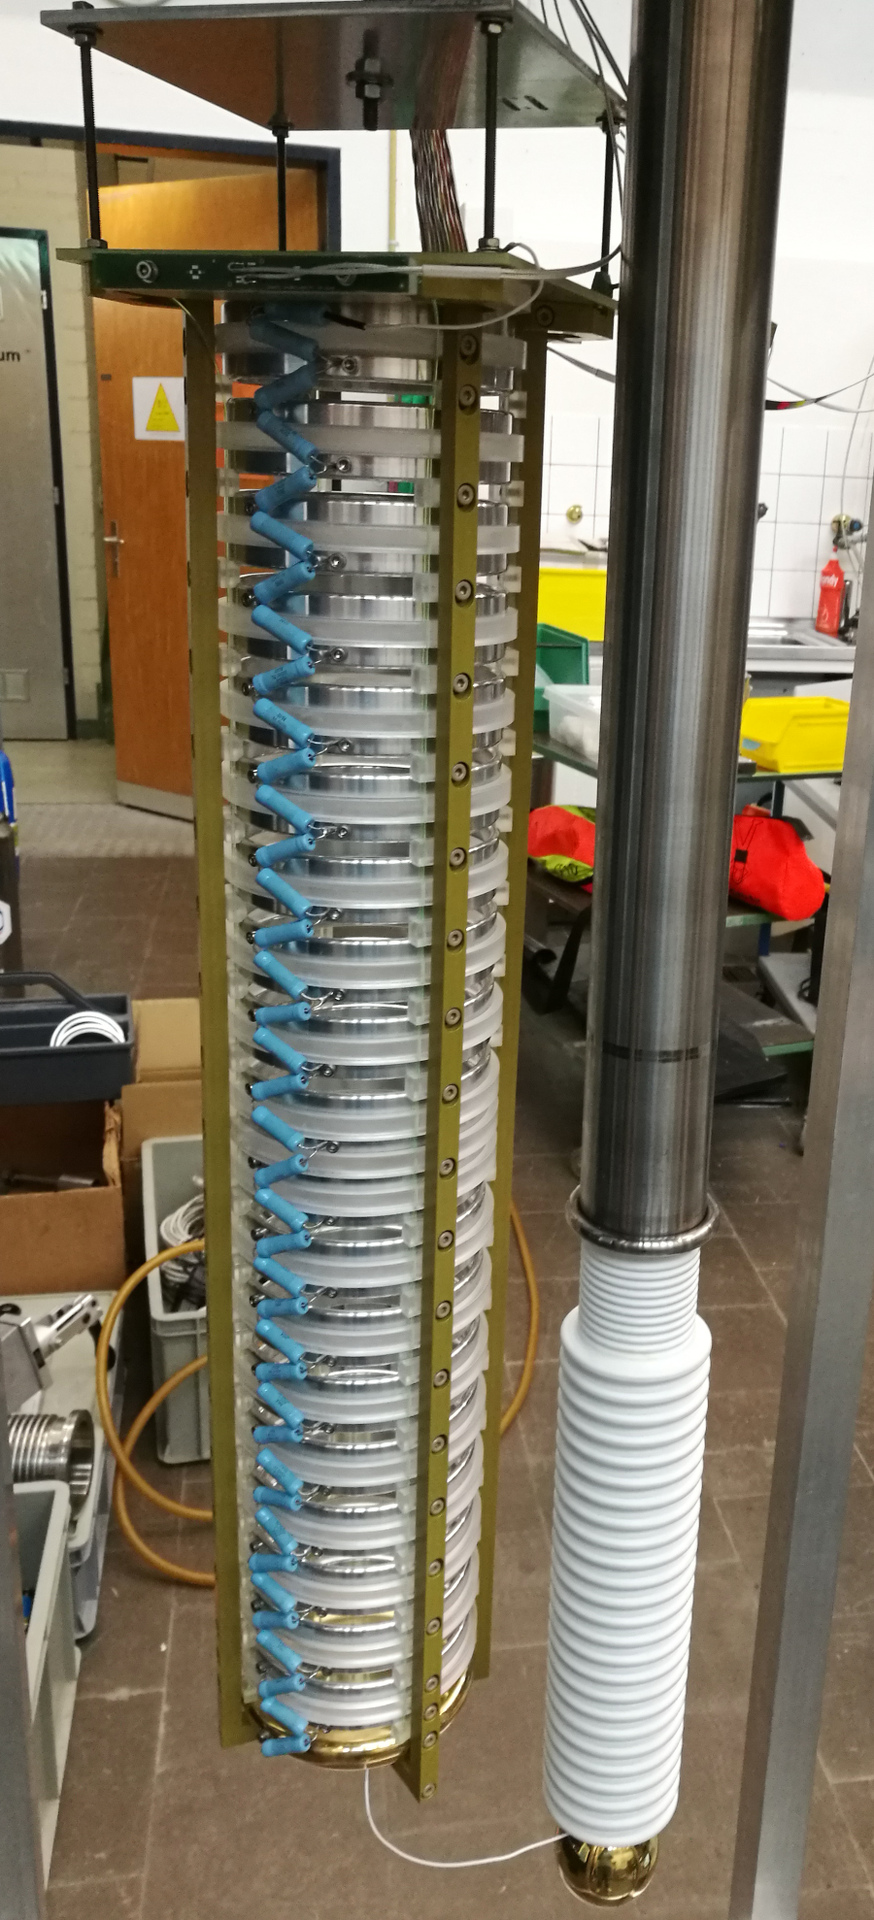
\includegraphics[height=.8\textheight]{viper/viper_original}
		\column{.4\textwidth}
		\centering
		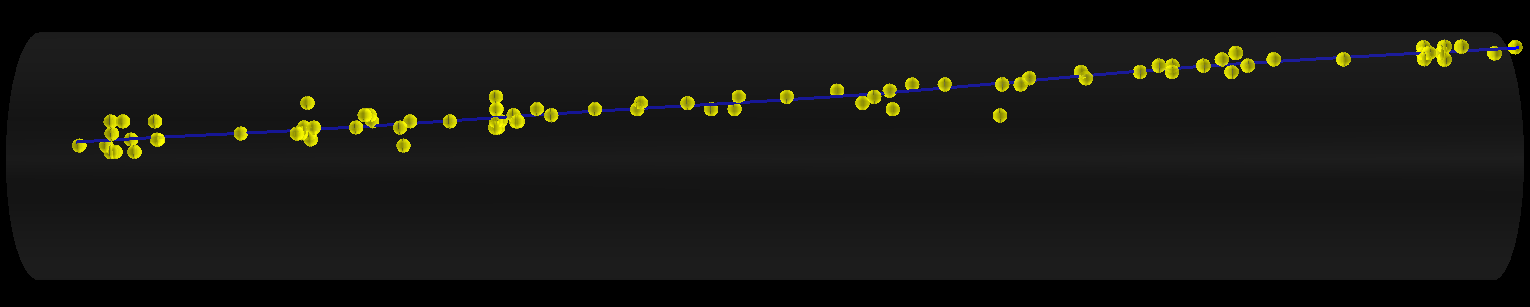
\includegraphics[width=.8\textheight, angle=90]{viper/event967_kalman}
	\end{columns}
	\centering
	{\tiny University of Bern, 2017}\\
\end{frame}

\begin{frame}{Step-by-step 3D event reconstruction}
	\begin{columns}[c]
		\column{.5\textwidth}
		\begin{enumerate}
			\item<1-> Noise filter
			\begin{itemize}
				\item Subtract common mode noise
			\end{itemize}
			\item<2-> Hit finder
			\item<2-> Hit matcher
			\begin{itemize}
				\item Combine pixel and ROI hits into 3D hits
			\end{itemize}
			\item<3-> Principal Component Analysis
			\begin{itemize}
				\item Solve multiplexing ambiguities (red)
				\item Remove outliers
			\end{itemize}
			\item<4-> Kalman fitter
			\begin{itemize}
				\item Fit $\mu$ hypothesis to 3D spacepoints
				\item GENFIT, arXiv:\\0911.1008~\cite{genfit1}, 1410.3698~\cite{genfit2}
			\end{itemize}
		\end{enumerate}
		\column{.5\textwidth}
		\centering
		\only<1>{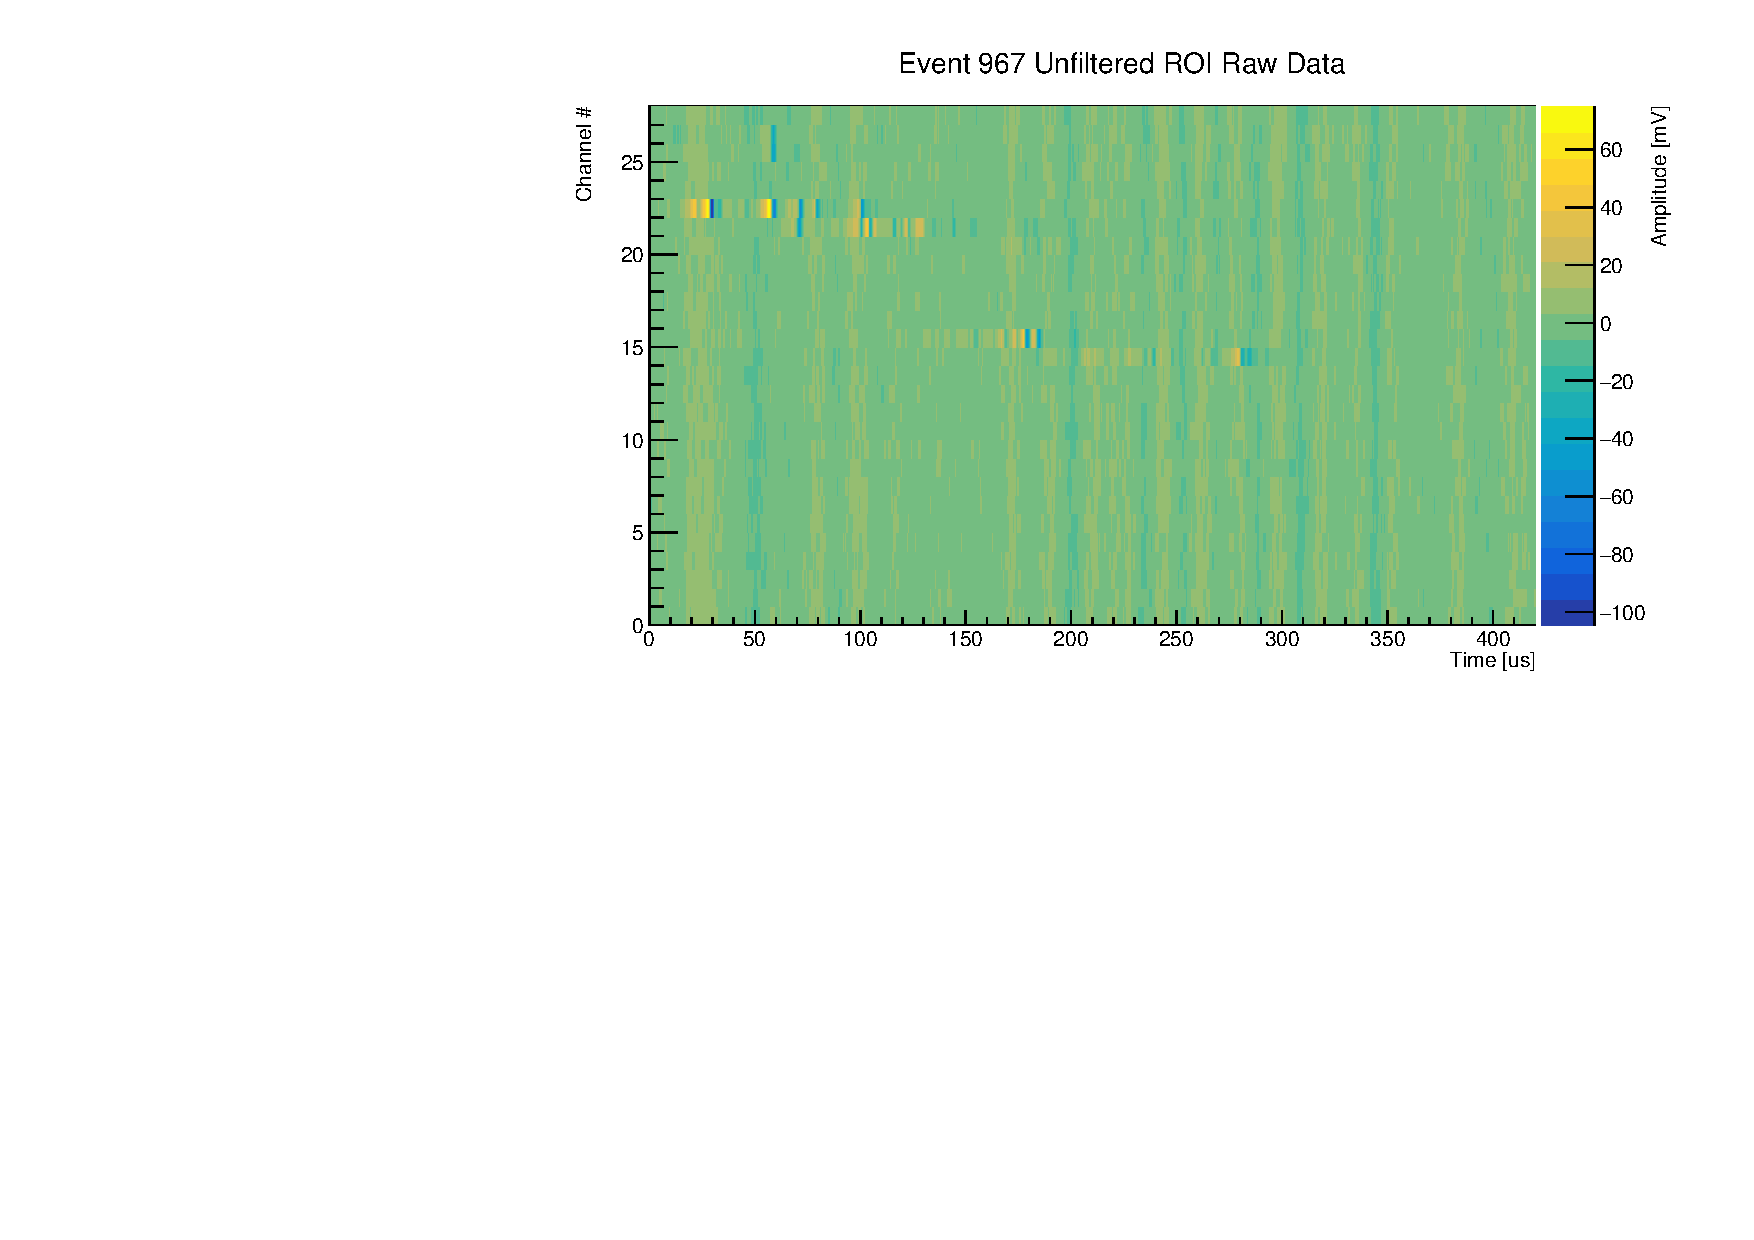
\includegraphics[height=.4\textheight]{viper/event967_rawUnfilteredROI}\\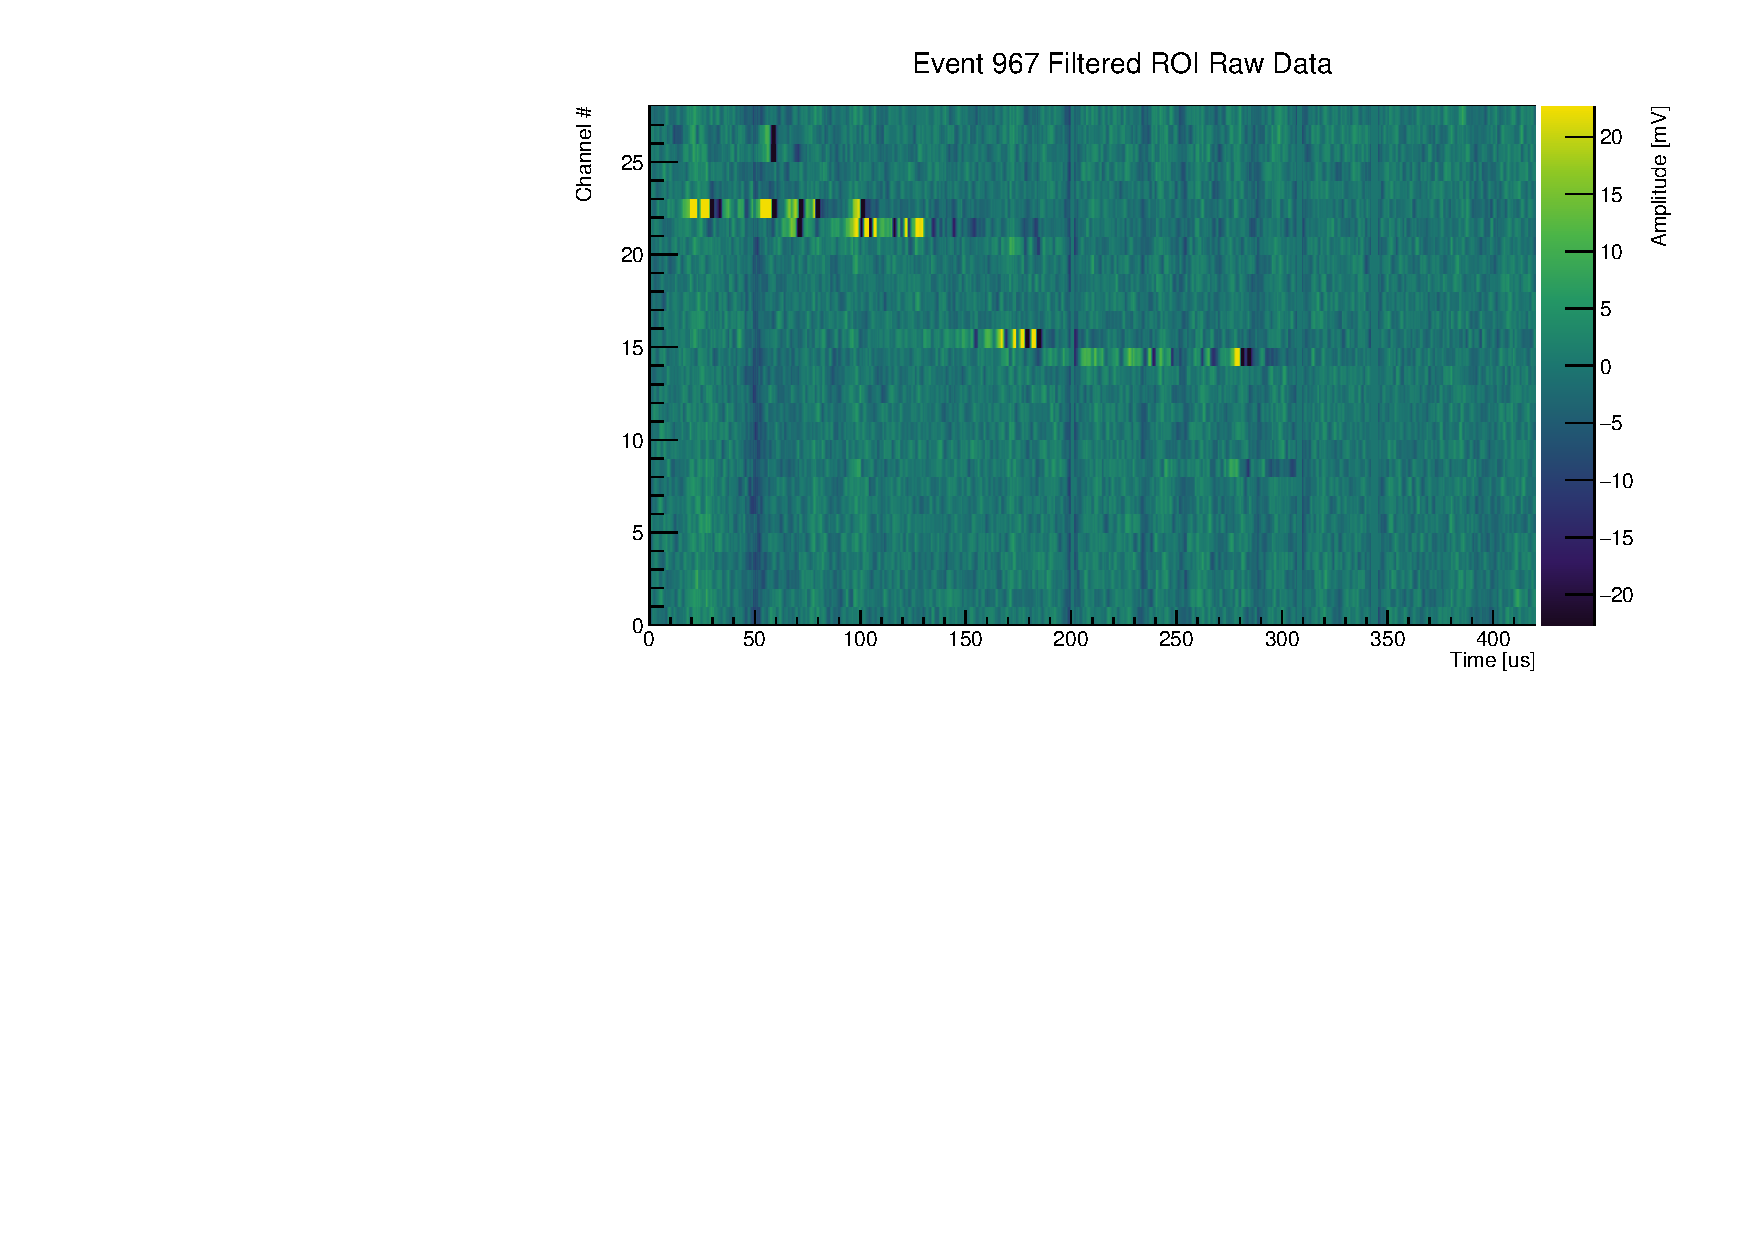
\includegraphics[height=.4\textheight]{viper/event967_rawFilteredROI}\\{\tiny University of Bern, 2017}\\}
		\only<2>{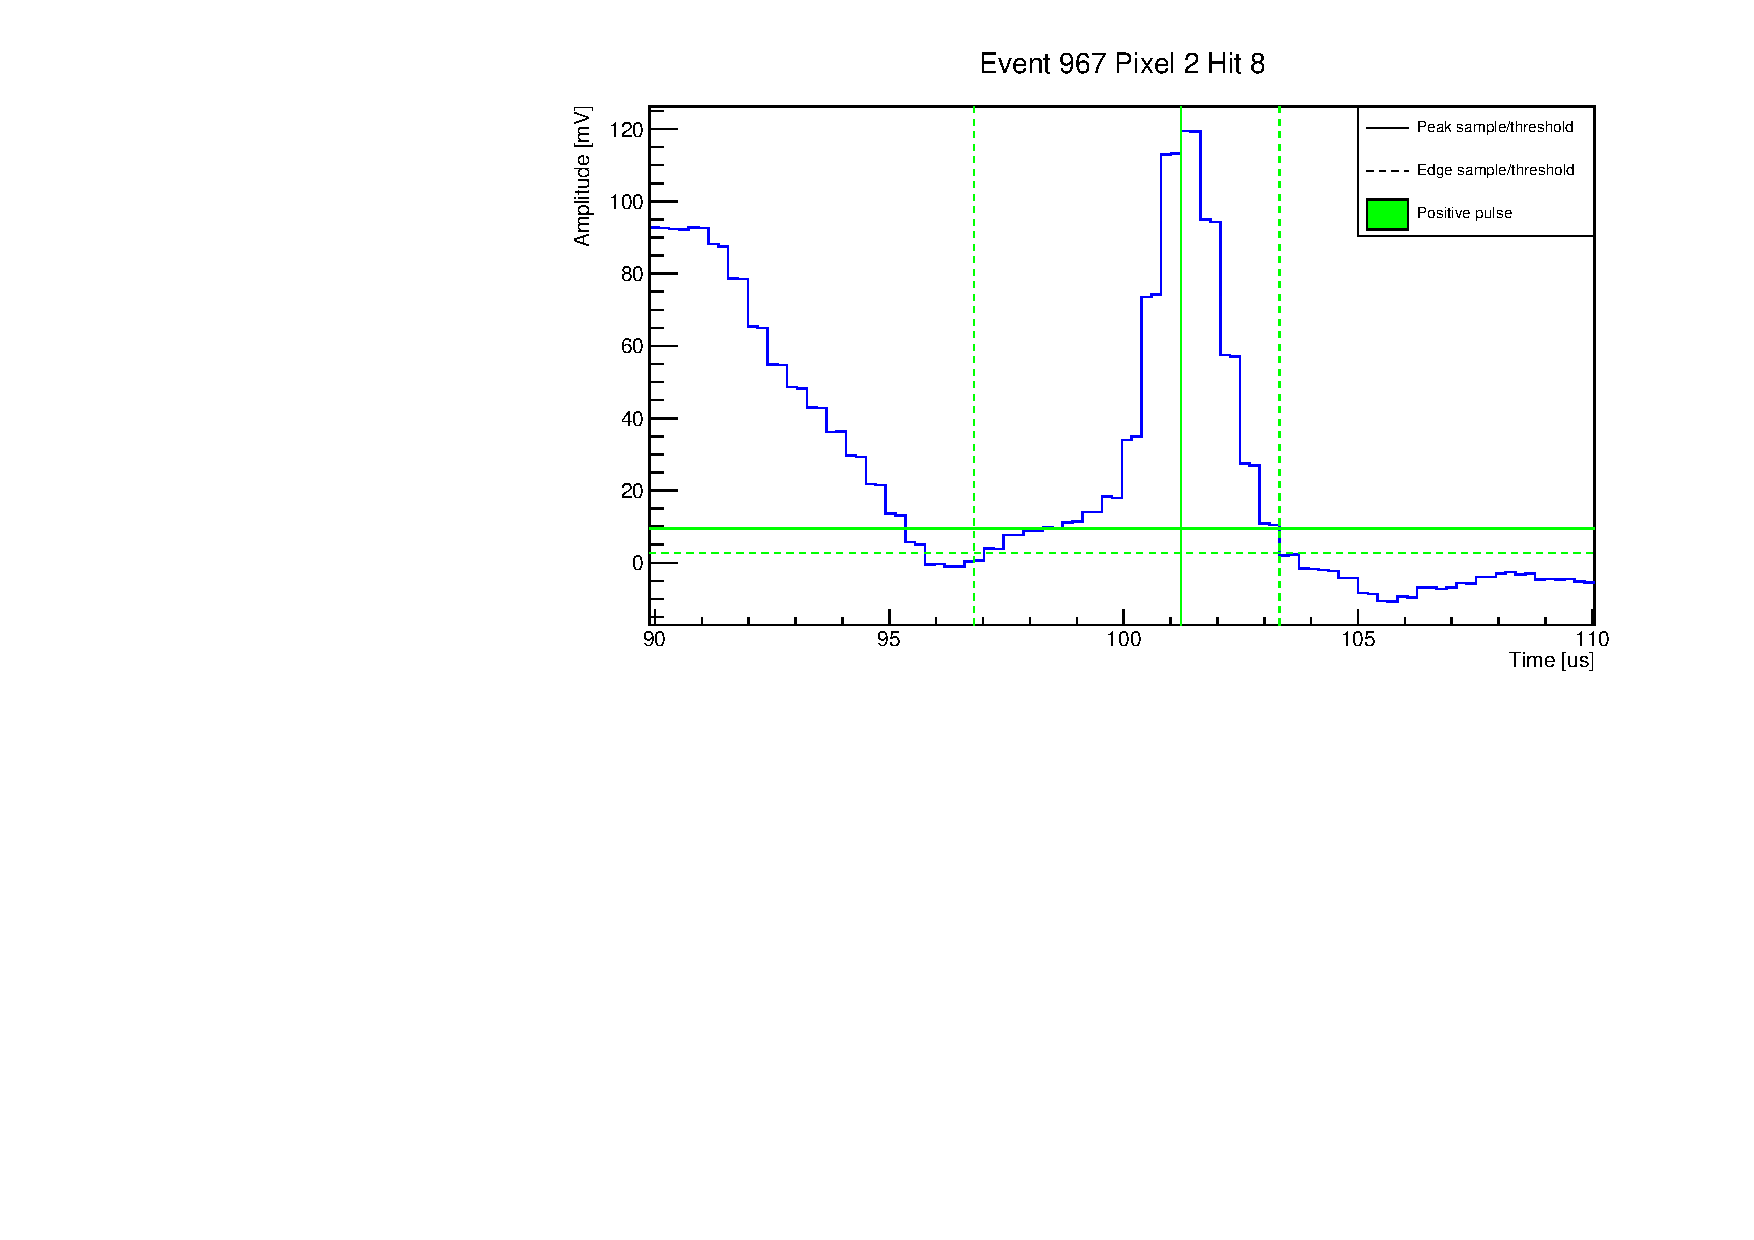
\includegraphics[page=1, height=.4\textheight]{viper/event967_pixel2_hit8}\\\includegraphics[page=3, height=.4\textheight]{viper/event967_pixel2_hit8}\\{\tiny University of Bern, 2017}\\}
		\only<3>{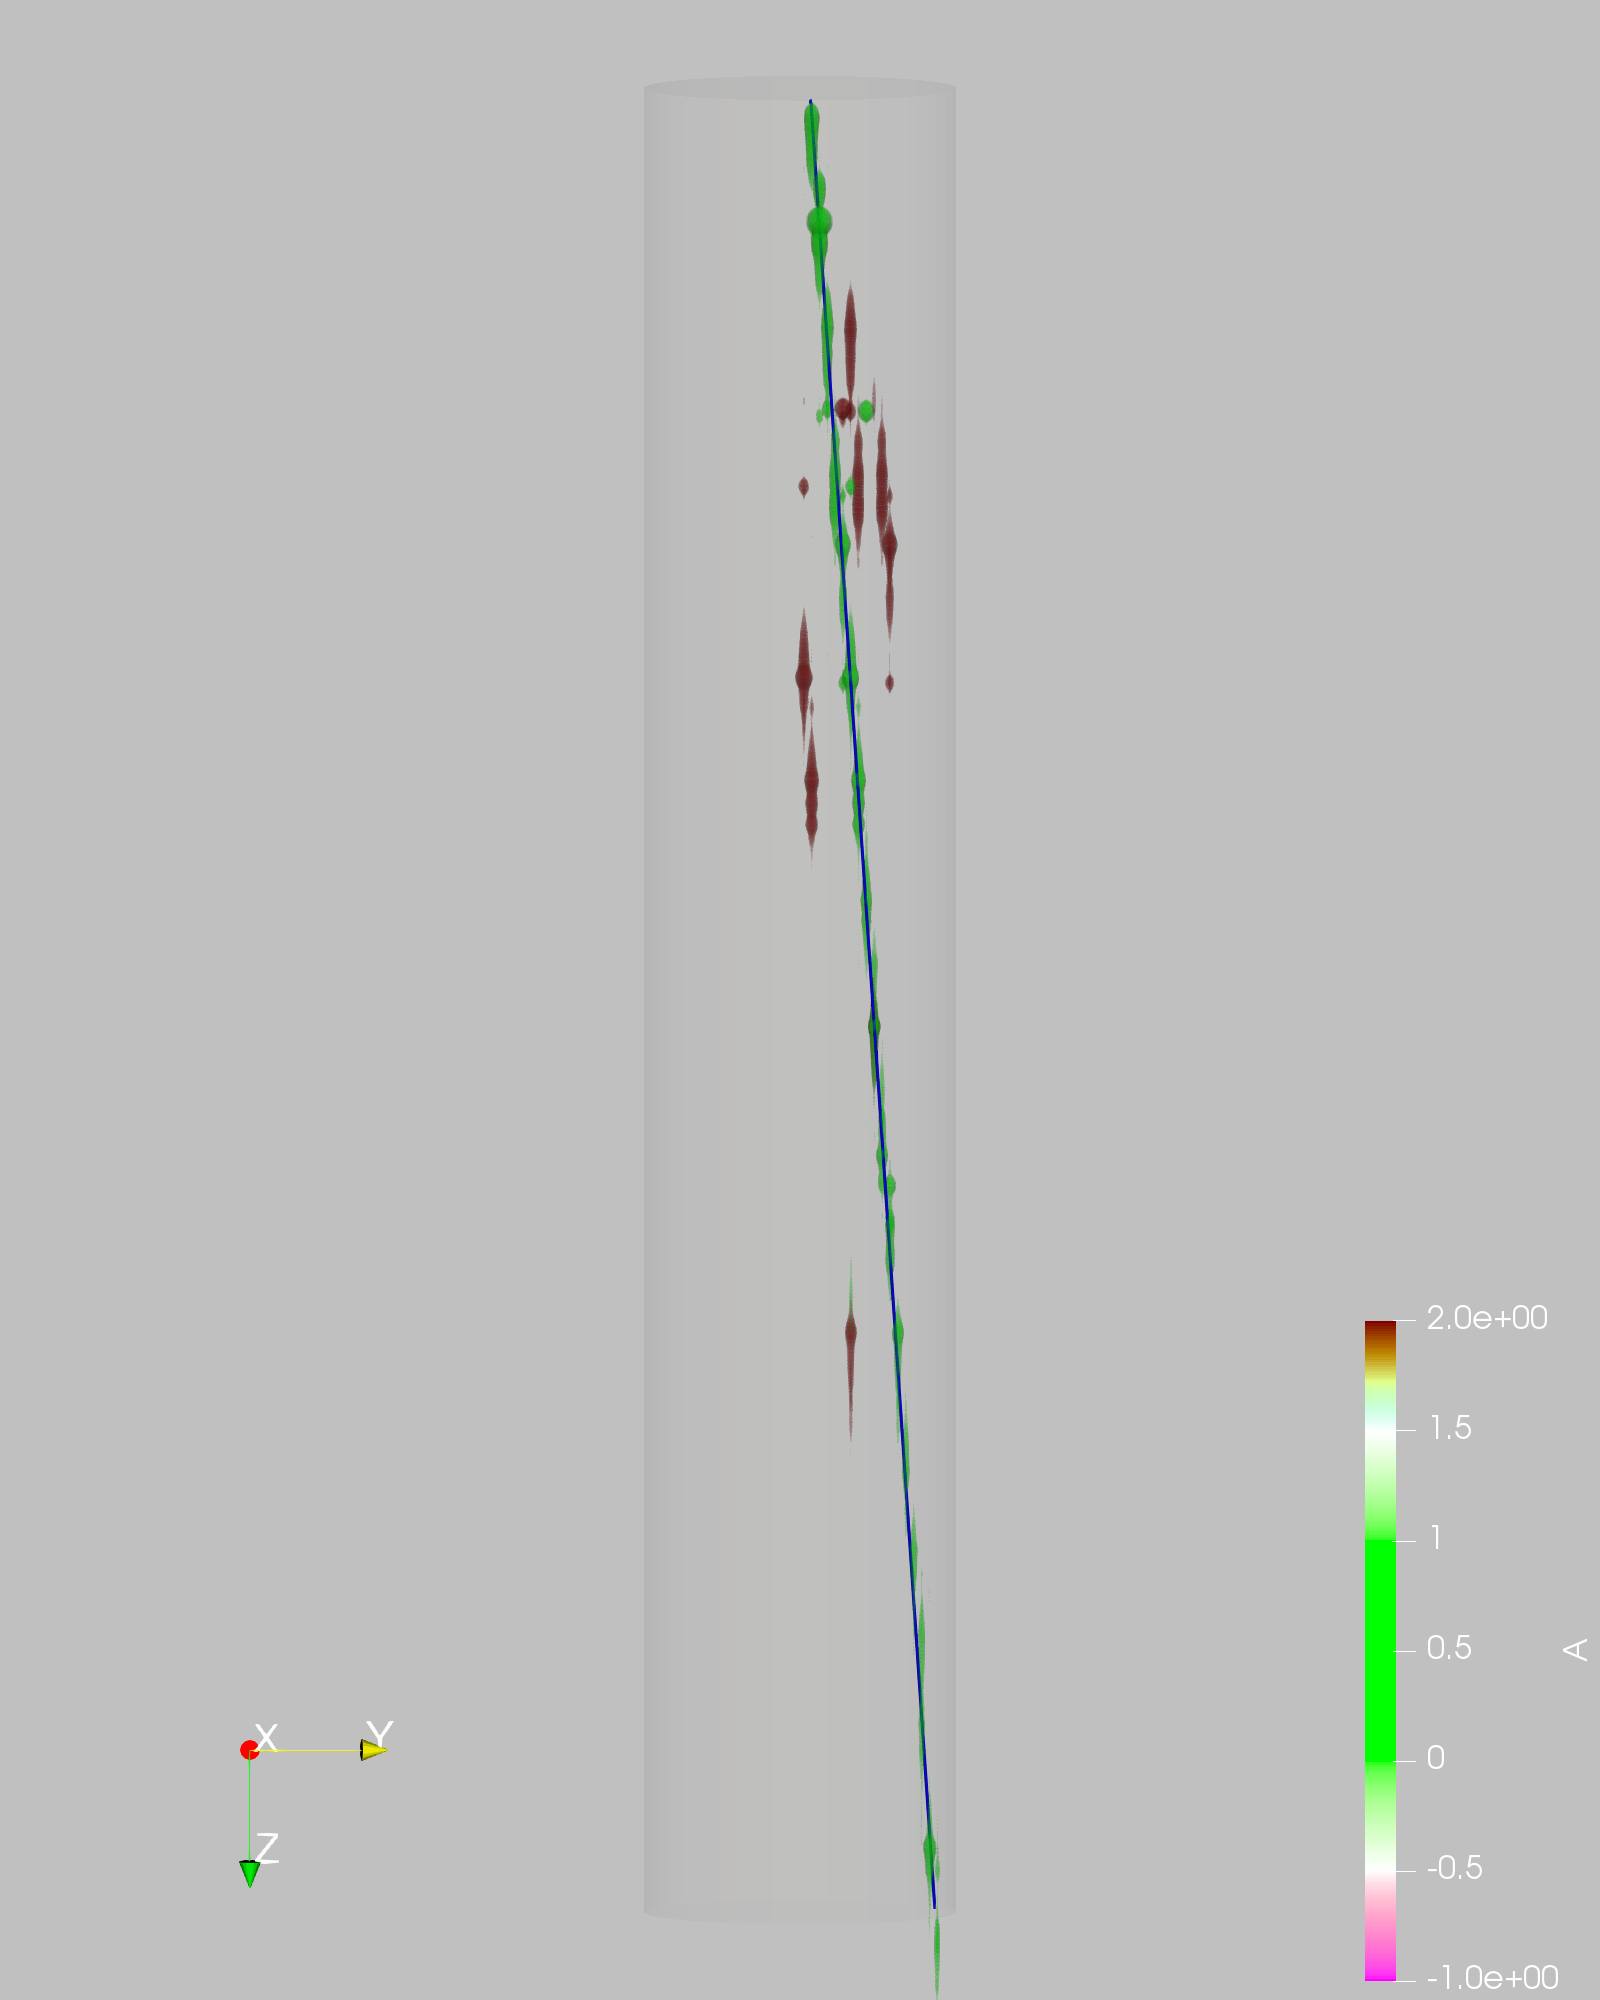
\includegraphics[height=.8\textheight]{viper/event967_pulses_a_pca}\\{\tiny University of Bern, 2017}\\}
		\only<4>{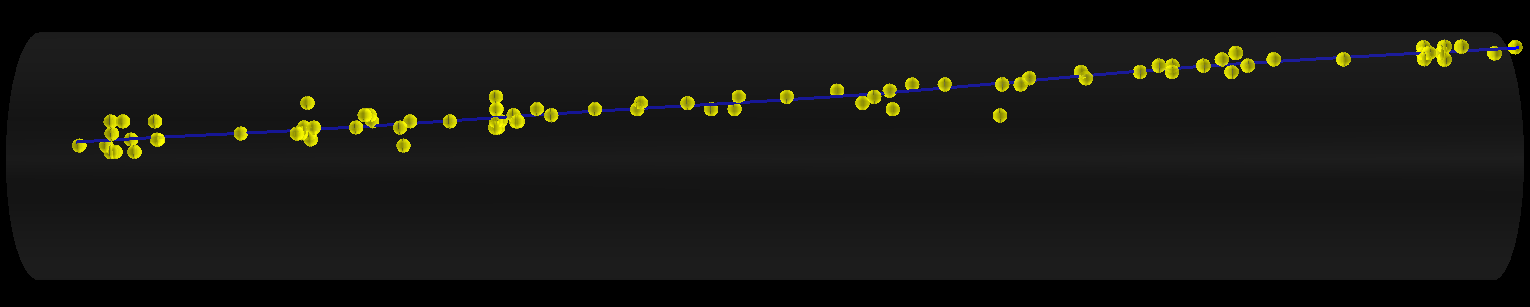
\includegraphics[width=.8\textheight, angle=-90]{viper/event967_kalman}\\{\tiny University of Bern, 2017}\\}
	\end{columns}
\end{frame}

\begin{frame}{Charge readout summary}{\color{\emphcol} Demonstrated a pixelated \lartpc{}, enabling true 3D tracking}
	\begin{columns}[c]
		\column{.5\textwidth}
		\centering
		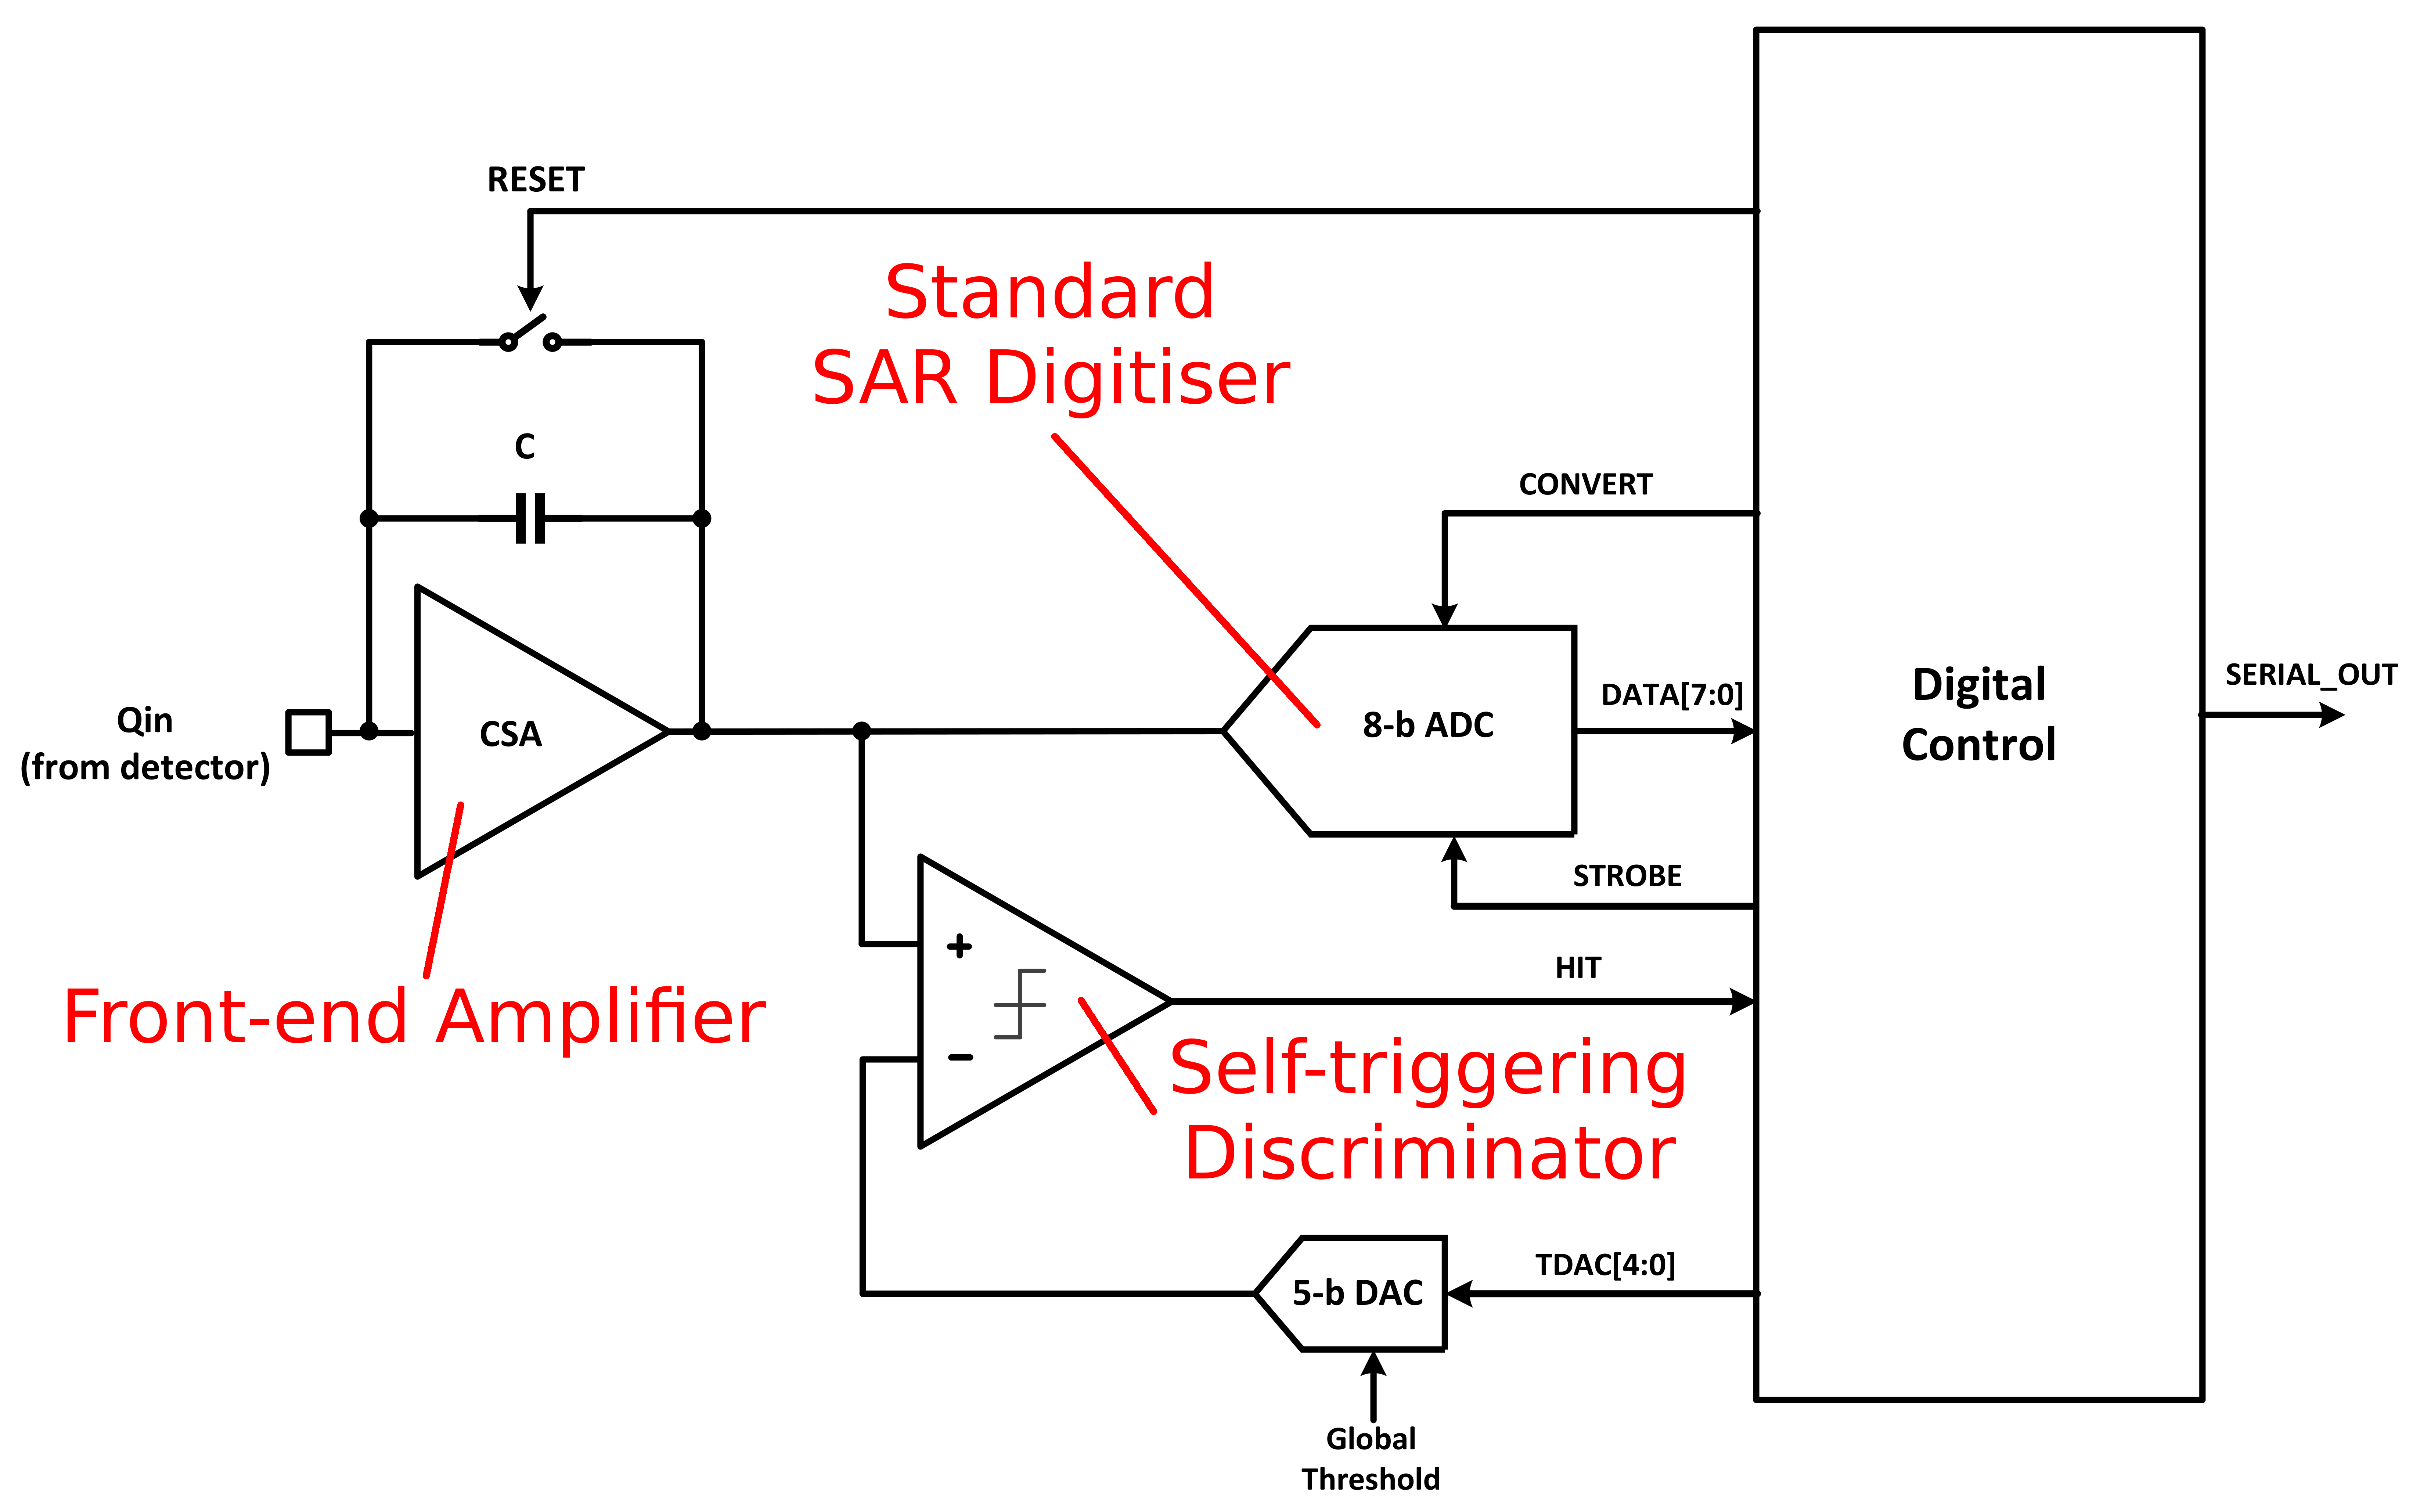
\includegraphics[width=\textwidth]{larpix/schematic}\\
		{\tiny University of Bern, 2017}\\
		\column{.5\textwidth}
		\begin{itemize}
			\item MIP signal-to-noise ratio: \num{14}
			\item Double-track spatial resolution in XY: \SI{2.54}{\milli\metre}
			\item Double-track spatial resolution in Z: \SI{2.1}{\milli\metre}
			\item Successfully reconstructed single tracks
			\item Potentially momentum and PID from Kalman
			\item {\color{\emphcol} Limited by multiplexing ambiguities}
			\item[$\Rightarrow$] {\color{\emphcol} New cold digitisers under development at LBNL}
		\end{itemize}
	\end{columns}
\end{frame}

\section{Light readout}

\begin{frame}{The standard \lartpc{} design}{Light readout}
	\centering
	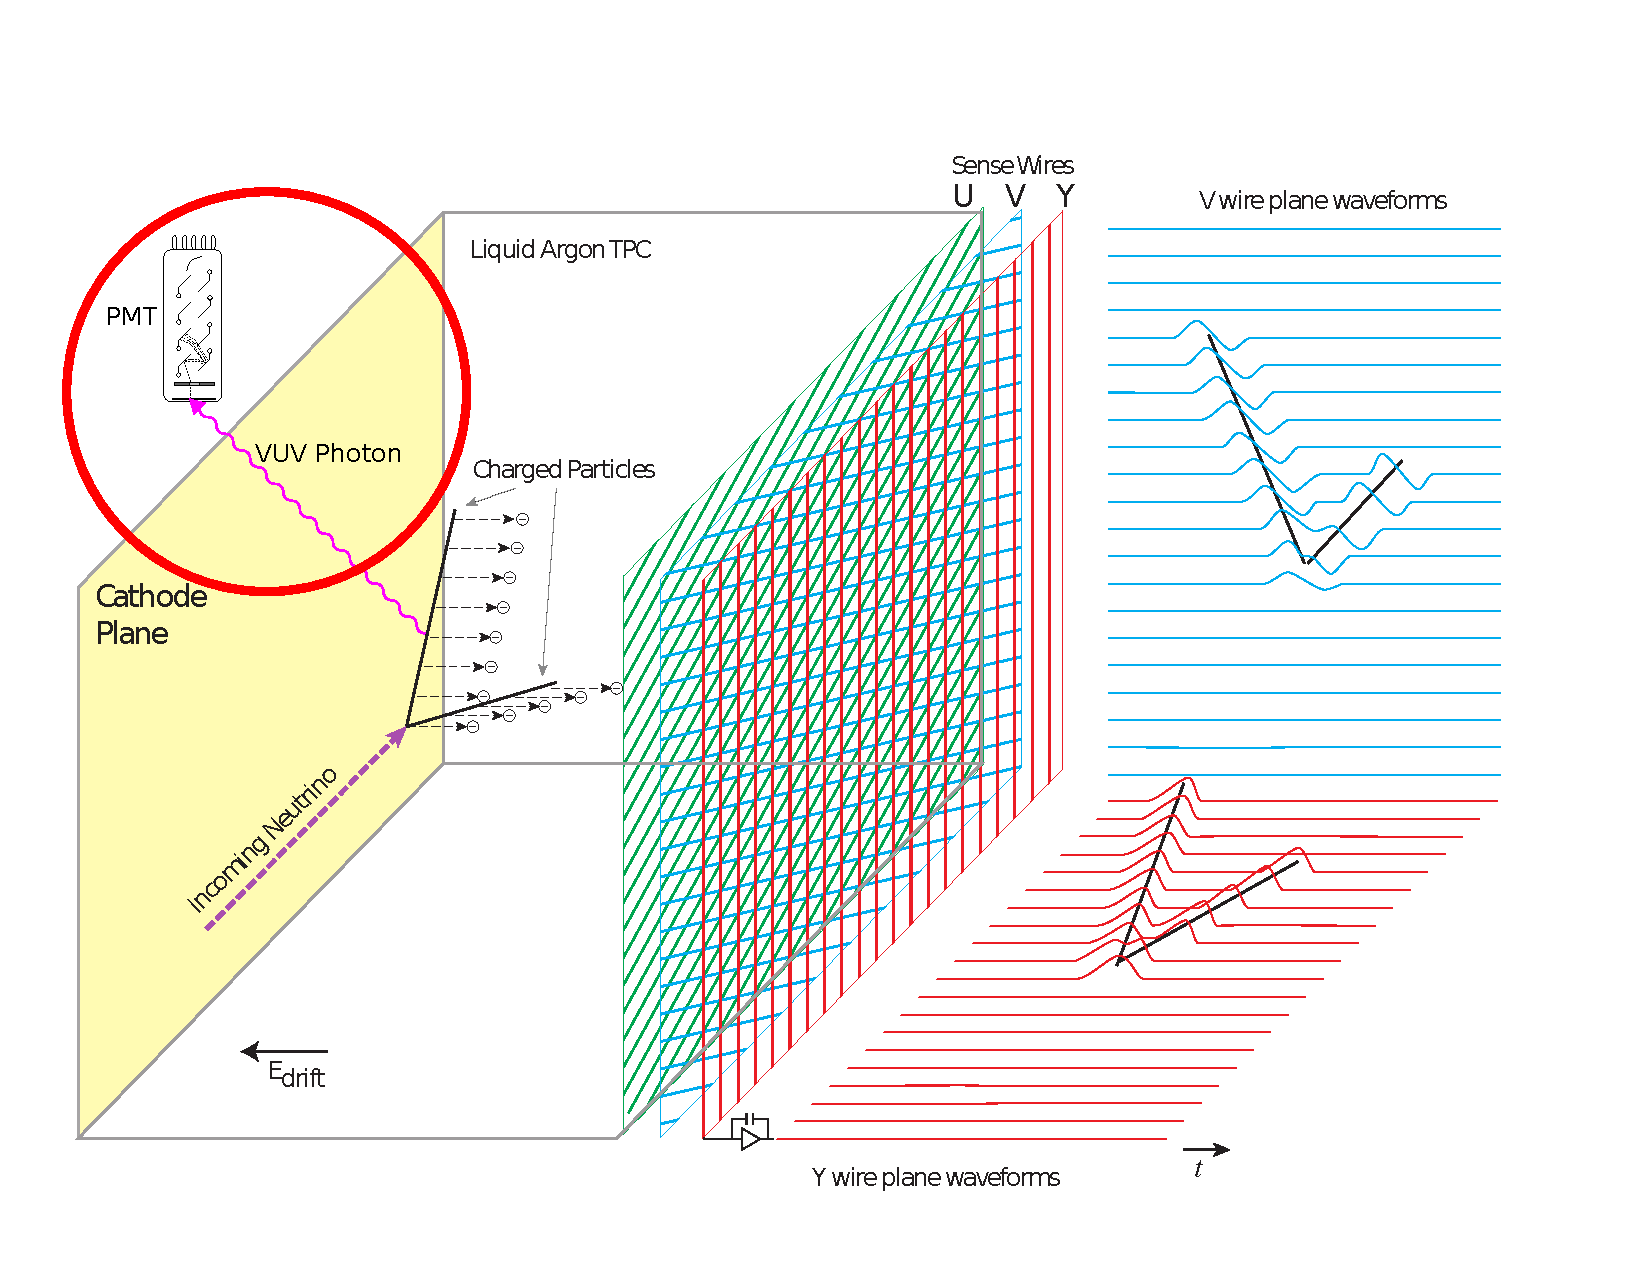
\includegraphics[viewport=30 40 720 540, clip, height=.66\textheight]{defence/TPCprinciple_light-ro}\\
	{\tiny \uboone{} arXiv:~1612.05824~\cite{uboone}}\\
\end{frame}

\begin{frame}{\AC{} Light readout system (\AL{})}{\color{\emphcol}A SiPM-based compact, robust, scalable \lartpc{} light readout}
	\centering
	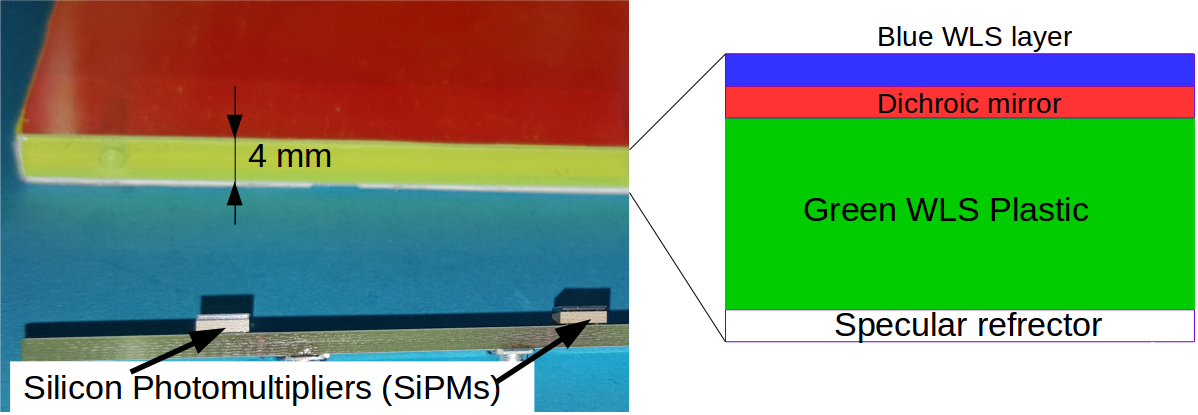
\includegraphics[width=\textwidth]{arclight/structure}
\end{frame}

\begin{frame}{\AL{} in operation}{\color{\emphcol} Stable operation over several weeks at \lar{} temperature}
	\centering
	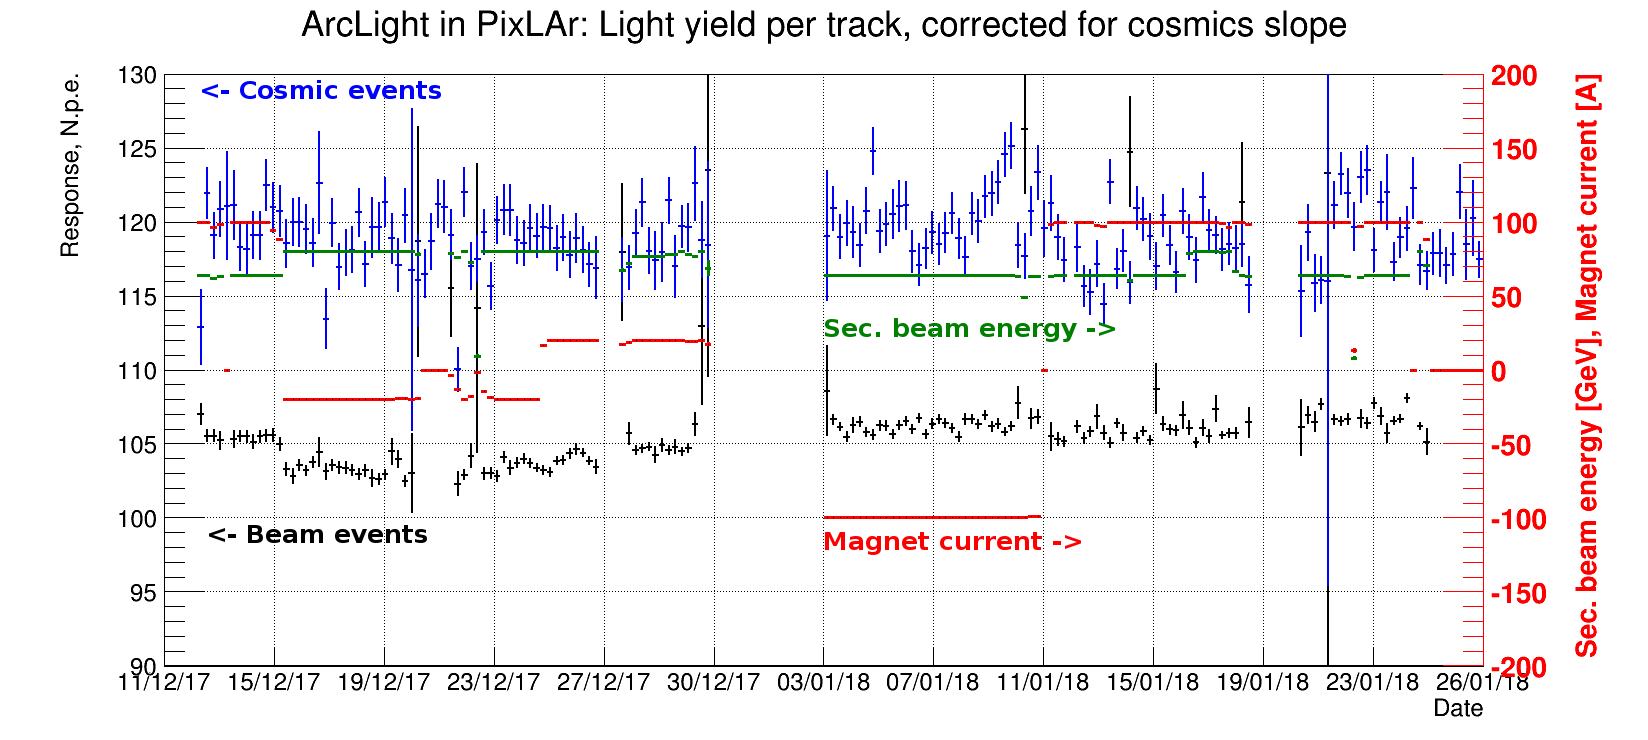
\includegraphics[viewport=0 0 1648 690, clip, width=\textwidth]{arclight/stability_cosm_beam_mod}
\end{frame}

\begin{frame}{Light readout summary}{\AL{}, a novel \lartpc{} light readout combining SiPMs with a light trap}
	\begin{columns}[c]
		\column{.5\textwidth}
		\centering
		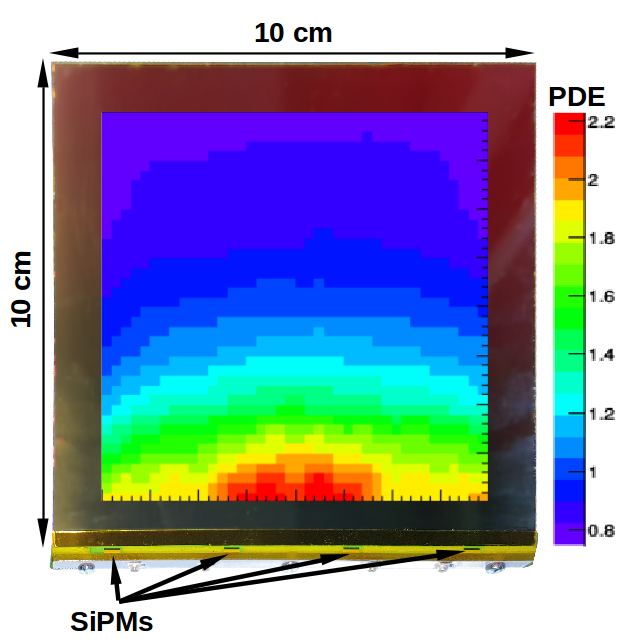
\includegraphics[width=\textwidth]{arclight/PDE}
		\column{.5\textwidth}
		\begin{itemize}
			\item SiPM-based light trap
			\item Compact
			\item Resilient to electric fields
			\item PDE \SI{\sim 1}{\percent}
			\item[$\Rightarrow$] Suited for a modular TPC design
			\item[$\Rightarrow$] {\color{\emphcol} Contained scintillation light enables localisation}
		\end{itemize}
	\end{columns}
\end{frame}

\section{\AC{}}

\begin{frame}{\AC{}}{\color{\emphcol}A scalable high-precision tracker and calorimeter based on self-contained \lartpc{}s}
	\begin{columns}[c]
		\column{.6\textwidth}
		\centering
		\includegraphics[width=\textwidth]{ac/2x2/Normal-Module-4K_labelled}
		\column{.4\textwidth}
		\begin{itemize}
			\item \SI{50}{\centi\metre} drift length
			\item[$\Rightarrow$] {\color{\emphcol} Safe cathode voltage}
			\item Pixelated charge readout
			\item[$\Rightarrow$] {\color{\emphcol} True 3D tracking}
			\item \AL{} readout
			\item[$\Rightarrow$] {\color{\emphcol} Reduce scintillation light pile-up}
		\end{itemize}
	\end{columns}
\end{frame}

\begin{frame}{\AC{} \dune{} near detector component}
	\centering
	\textbf{\textrightarrow{}\textrightarrow{}\textrightarrow{}} Beam direction \textbf{\textrightarrow{}\textrightarrow{}\textrightarrow{}}
	\begin{columns}[c]
		\column{.5\textwidth}
		\centering
		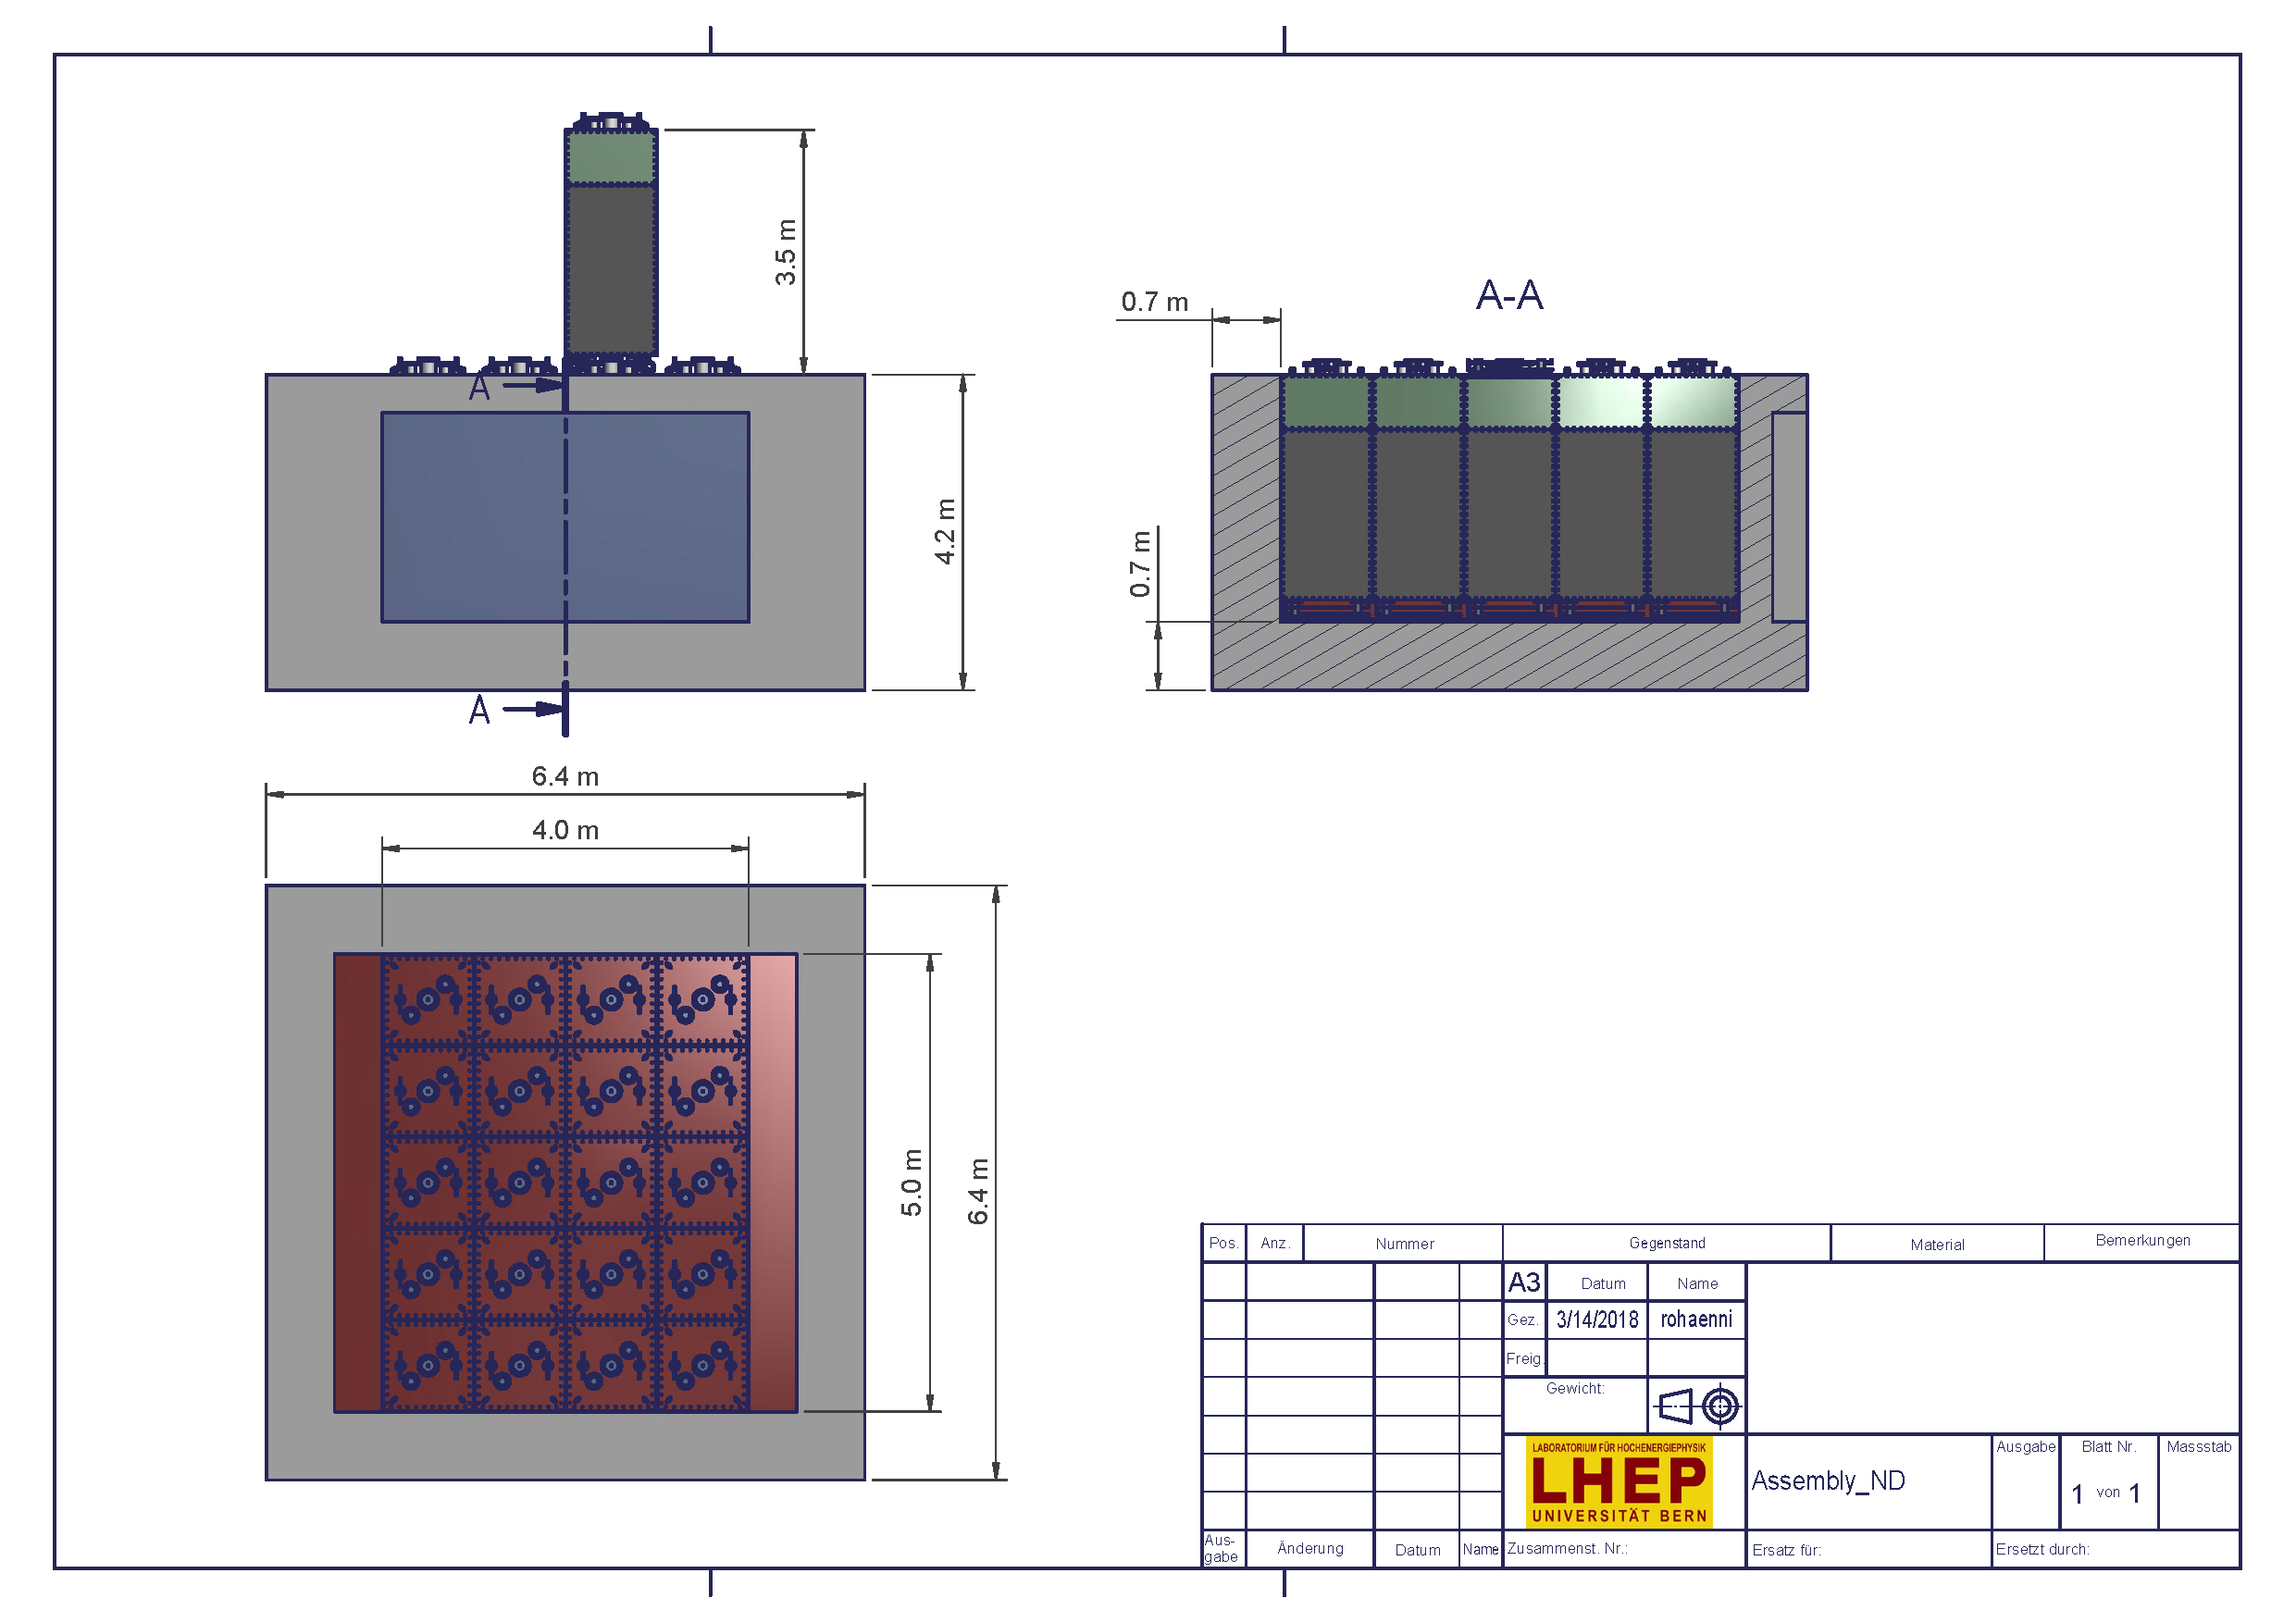
\includegraphics[viewport=130 70 530 450, clip, height=\textwidth, angle=-90]{ac/dune_nd/Assembly_ND-1}
		\column{.5\textwidth}
		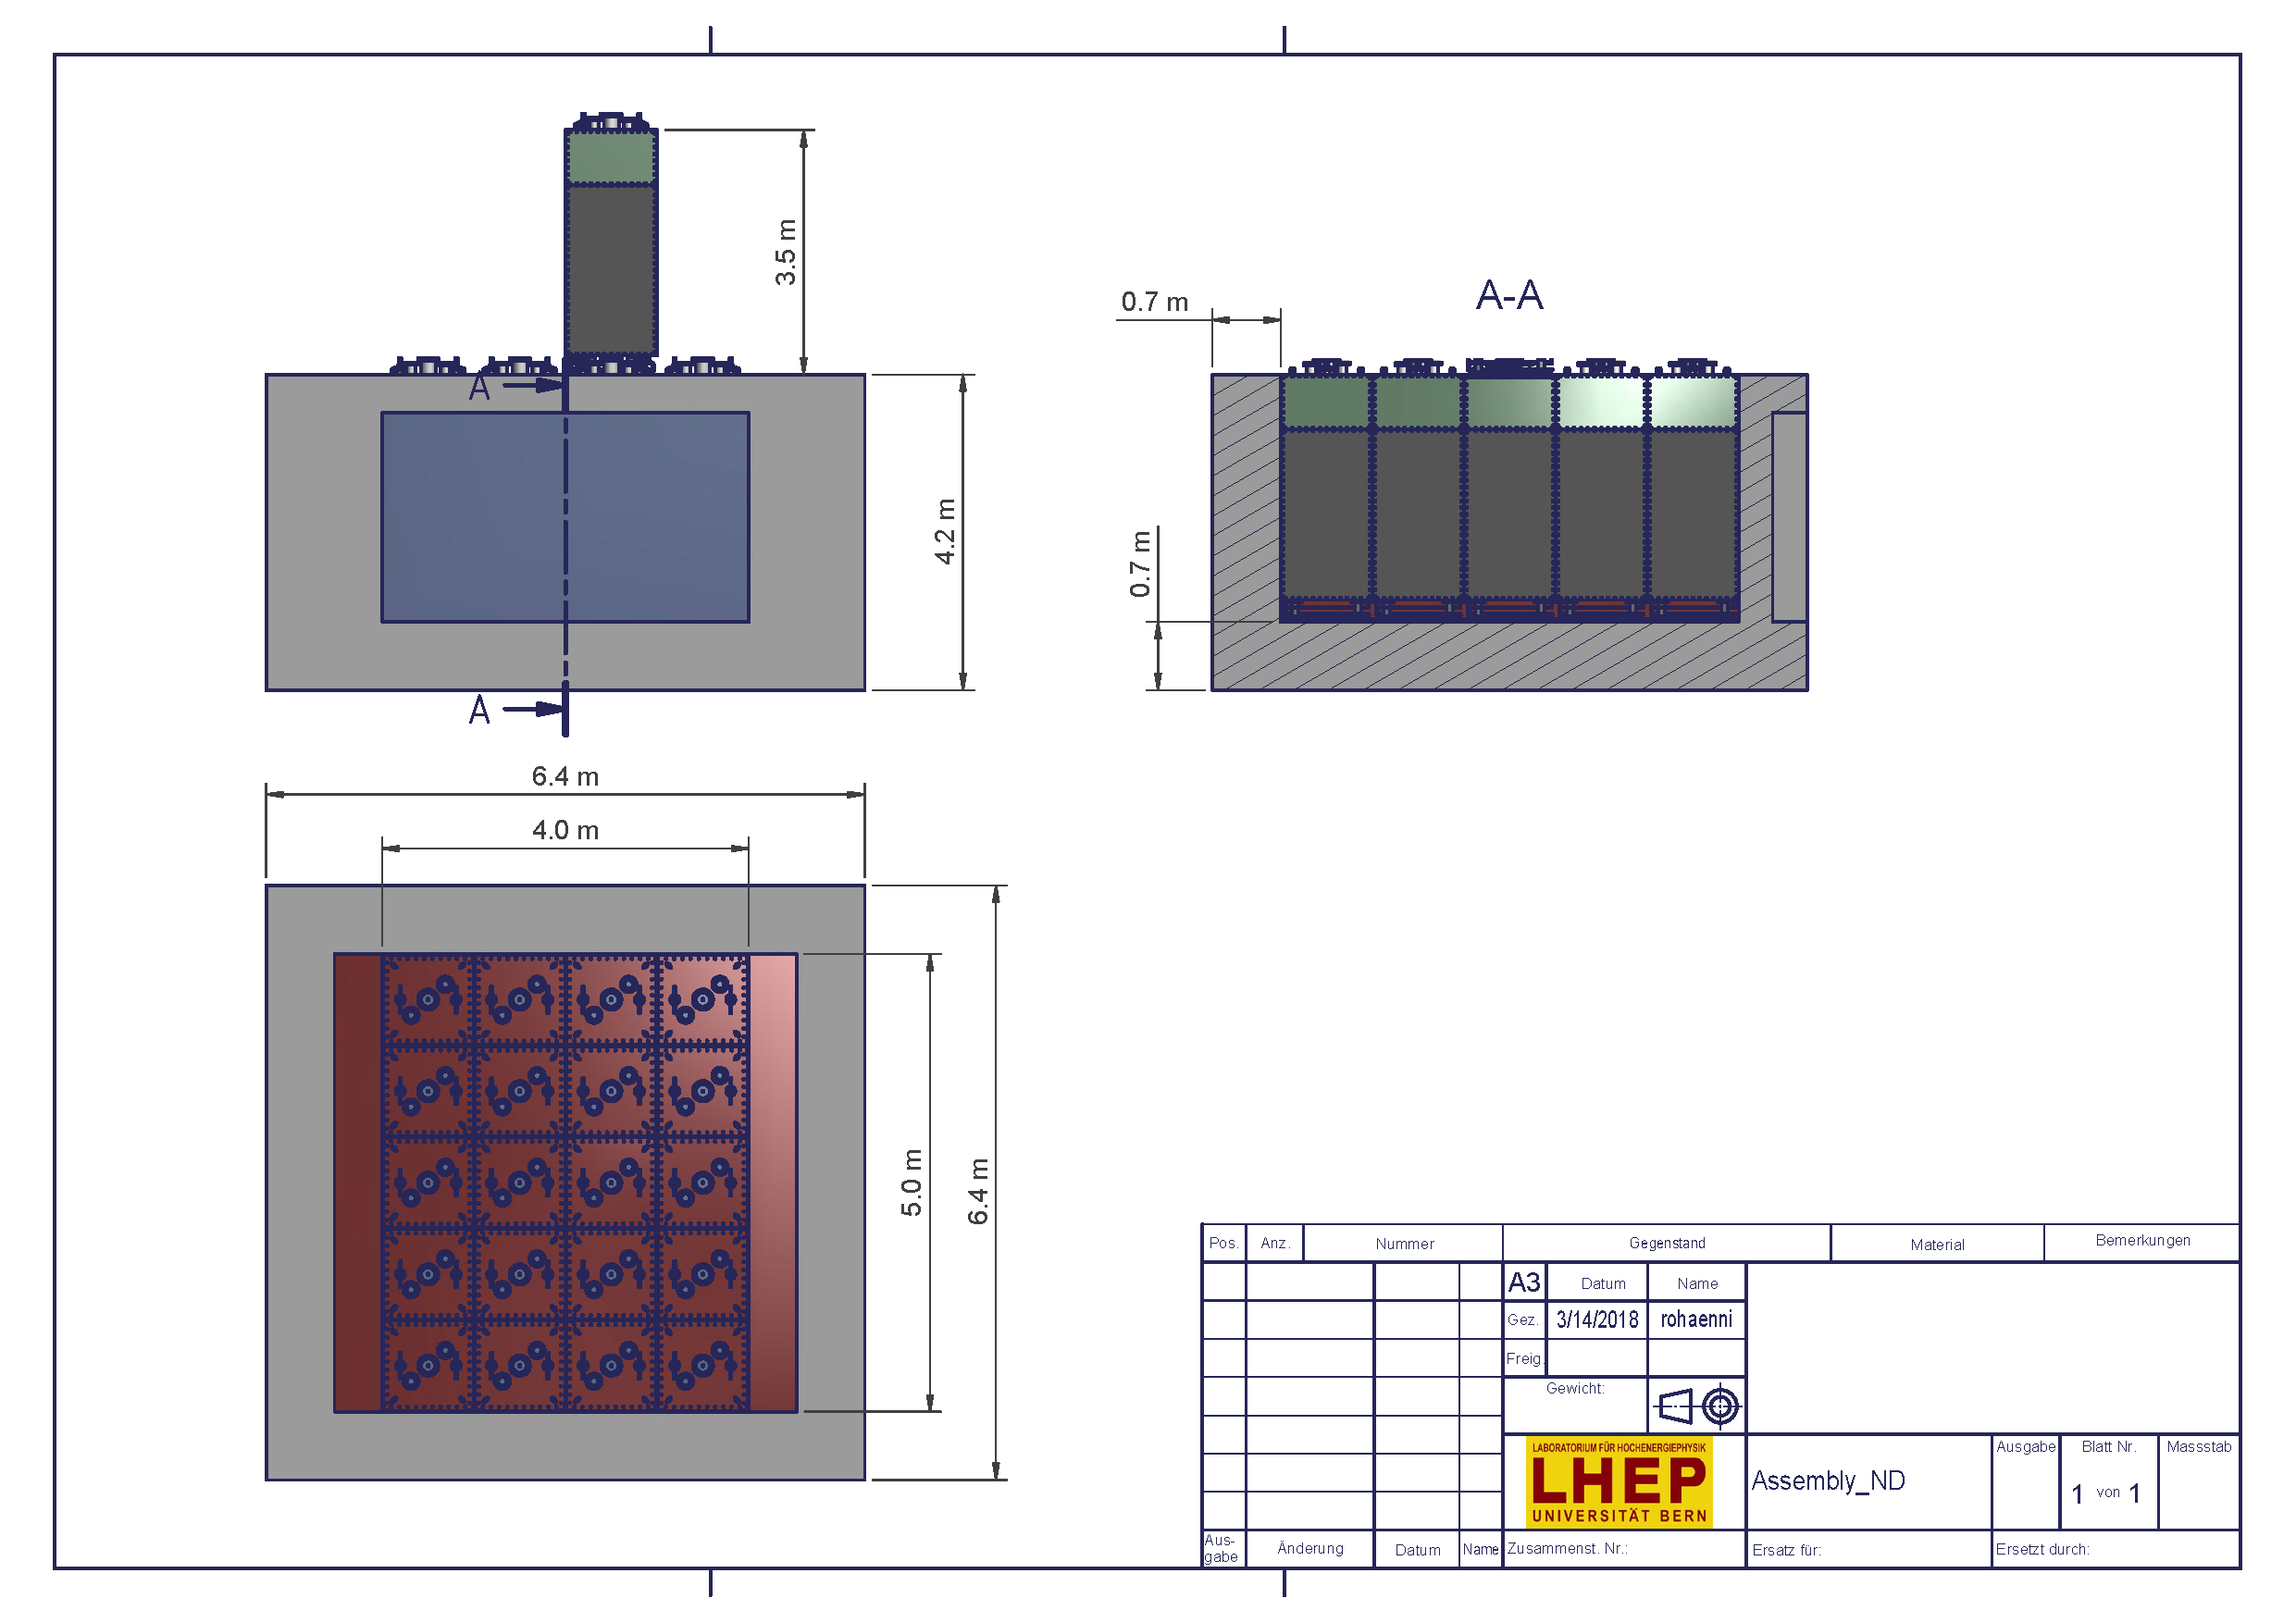
\includegraphics[viewport=580 480 940 700, clip, width=\textwidth]{ac/dune_nd/Assembly_ND-1}
	\end{columns}
\end{frame}

\section{Event pile-up}

\begin{frame}{Can a pixelated \AC{} \dune{} near detector cope with the expected event rates?}
	\begin{columns}[c]
		\column{.5\textwidth}
		\centering
		\includegraphics[width=\textwidth]{defence/uboone_em-shower_gamma}
		\column{.5\textwidth}
		\begin{itemize}
			\item \SIrange{10}{20}{\percent} of events involve \Pgpz
			\item \HepProcess{\Pgpz \to \Pgg\Pgg} \textrightarrow{} EM shower
			\item Lots of tiny charge clusters
			\item Missed/misidentified charge degrades energy resolution
			\item One of the most challenging reconstruction tasks
		\end{itemize}
	\end{columns}
\end{frame}

\begin{frame}{Event pile-up simulation}{For \AC{} in the \dune{} near detector}
	\begin{columns}[c]
		\column{.6\textwidth}
		\centering
		\includegraphics[viewport=2900 1800 4000 2600, clip, width=\textwidth]{pile-up/uid0_spill6_event461_gamma19_x}
		\column{.4\textwidth}
		\begin{itemize}
			\item Assume shower location and direction are known
			\item Form cone around shower
			\item Misidentified energy: Not deposited by shower, inside cone
			\item[$\Rightarrow$] Measure for pile-up
		\end{itemize}
	\end{columns}
\end{frame}

\begin{frame}{Misidentified energy}{Gauging event pile-up}
	\centering
	\includegraphics[width=\textwidth]{pile-up/2MW/misid_rel_x}
\end{frame}

\begin{frame}{Misidentified energy}{Gauging event pile-up}
	\centering
	\includegraphics[width=\textwidth]{pile-up/2MW/misid_rel_y}
\end{frame}

\begin{frame}{\AC{} summary}
	\begin{columns}[c]
		\column{.5\textwidth}
		\centering
		\includegraphics[width=.8\textheight, angle=90]{ac/2x2/module_real}
		\column{.5\textwidth}
		\begin{itemize}
			\item {\color{\emphcol} Enables a \lartpc{} component in the \dune{} near detector}
			\item Mean pile-up-related error on reconstructed energy: \SIrange{2}{3}{\percent}
			\item \SI{<0.1}{\percent} for \SI{>50}{\percent} of neutrino events
		\end{itemize}
	\end{columns}
\end{frame}

\appendix

\section{Backup}

\begin{frame}{Pixelated charge readout}{\color{\emphcol} Enabling true 3D tracking}
	\begin{columns}[c]
		\column{.5\textwidth}
		\centering
		\includegraphics[width=\textwidth]{viper/pixies}\\
		{\tiny University of Bern, 2016}\\
		\column{.5\textwidth}
		\begin{itemize}
			\item Charge collecting pixels
			\begin{itemize}
				\item[$\hookrightarrow$] PCB VIAs
				\item Low capacitance
				\item[$\Rightarrow$] Reduce Johnson-Nyquist noise $Q_{\m{Noise}} = \sqrt{k_{\m{B}}TC}$
			\end{itemize}
			\item Biased charge focussing grids
			\begin{itemize}
				\item[$\hookrightarrow$] PCB traces
			\end{itemize}
		\end{itemize}
	\end{columns}
\end{frame}

\begin{frame}{Cold charge amplifiers}{\color{\emphcol} Warm vs.\ cold}
	\centering
	\includegraphics[width=\textwidth]{defence/AT_warmPreamps}\\
	\includegraphics[width=\textwidth]{defence/AT_coldPreamps}\\
	{\tiny Ereditato, Goeldi et al.\ arXiv:~1408.7046~\cite{larasic}}\\
\end{frame}

\begin{frame}{Cold charge ADCs}{\color{\emphcol} Linearity issues with current designs}
	\centering
	\includegraphics[height=.8\textheight]{bnl/bnl_adc_lin}
\end{frame}

\begin{frame}{Regions of interest (ROI) multiplexing}
	\begin{columns}[c]
		\column{.4\textwidth}
		\centering
		\includegraphics[width=\textwidth]{defence/roi}\\
		{\tiny Igor Kreslo, University of Bern}\\
		\column{.6\textwidth}
		\begin{itemize}
			\item Number of physical pixels: {\color{\emphcol} $n_{\m{ROI}} * n_{\m{Pixel}}$}
			\item Number of DAQ channels: {\color{\emphcol} $n_{\m{ROI}} + n_{\m{Pixel}}$}
			\item For a square readout plane with a side length of $N$ physical pixels:
			\item $N ^ 2$ physical pixels
			\item $2 N$ DAQ channels
			\begin{itemize}
				\item[$\Rightarrow$] Same as 2-plane wire readout of equal size and pitch
			\end{itemize}
		\end{itemize}
	\end{columns}
\end{frame}

\begin{frame}{Missing energy}{Gauging reconstruction efficiency}
	\centering
	\includegraphics[width=\textwidth]{pile-up/2MW/missed_rel_x}
\end{frame}

\end{document}